\section{Valutazione euristica}
\label{subsec:valutazione_euristica}

\subsection{Fase preliminare}
Durante la fase preliminare del progetto, abbiamo definito e organizzato tutti gli aspetti necessari alla successiva fase di analisi.

In primo luogo abbiamo progettato l'esperienza descrivendo in modo dettagliato l'oggetto di studio. In questa fase abbiamo pianificato l'organizzazione temporale delle attività, definendo le scadenze e la distribuzione dei compiti all'interno del gruppo.

Successivamente, abbiamo definito le condizioni sperimentali, individuando come profilo utente di riferimento lo \textit{studente universitario}, in quanto principale destinatario e utilizzatore del sistema.

Infine, abbiamo esplicitato l'insieme dei principi euristici adottati, scegliendo di basarci sui principi di Nielsen, che ci guideranno nella valutazione dell'usabilità del sistema. \\

\noindent
Di seguito sono riportati i \textbf{dieci principi euristici di Nielsen} (rielaborati da \textit{P.Mussio}):

\begin{enumerate}
	\item Far vedere lo stato del sistema
	\item Adeguare il sistema al mondo reale
	\item Controllo dell'utente e libertà
	\item Assicurare consistenza
	\item Riconoscimento piuttosto che uso della memoria dell'utente
	\item Assicurare flessibilità ed efficienza d'uso
	\item Visualizzare tutte e sole le informazioni necessarie
	\item Prevenire gli errori
	\item Permettere all'utente di correggere gli errori e non solo di rilevarli
	\item Help e documentazione
\end{enumerate}

% -----------------------------------------------------
\subsection{Fase di esecuzione dell'analisi}
In questa seconda fase, ogni valutatore ha condotto in modo autonomo l'analisi euristica, individuando i problemi di usabilità riscontrati e indicando per ciascuno i principi di Nielsen violati. È stato deciso di dedicare a questa attività circa una settimana e mezza, così da consentire ai valutatori di svolgere l'analisi in sessioni differenti e aumentare le probabilità di individuare un numero maggiore di problemi.

Al termine delle valutazioni individuali, sono stati unificati i problemi simili ed eliminati gli eventuali duplicati, è stato assegnato un \textit{grado di severità} a ciascun problema e sono stati confermati i principi violati. Infine, sono stati elaborati i grafici di classificazione dei problemi presentati nelle sezioni successive di questo capitolo.

% -----------------------------------------------------
\subsection{Fase di debriefing}

\subsubsection{Elenco dei problemi individuati}
% TABELLE DEI PROBLEMI DI USABILITA'
% Problema \getNumeroProblema
\begin{table}[htbp]
  \centering
  \renewcommand{\arraystretch}{1.5}
  \begin{tabular}{|>{\raggedright\arraybackslash}p{7.5cm}|>{\raggedright\arraybackslash}p{7.5cm}|}
    \hline
    \rowcolor{green!30}
    \multicolumn{2}{|c|}{\textbf{Problema \getNumeroProblema}} \\
    \hline
    \textbf{Descrizione} & Il pulsante "Inizia Subito" in alto a destra dovrebbe essere "Registrati" per coerenza con "Accedi". \\
    \hline
    \textbf{Pagina del sito} & Homepage \\
    \hline
    \textbf{Principi violati} & 4 (Assicurare consistenza) \\
    \hline
    \textbf{Grado di severità} & 1 (Problema accessorio) \\
    \hline
    \textbf{Screen} &
    \vspace{10pt}
    \hspace*{\fill}
\includegraphics[width=6.5cm]{Screenshots/foglio1/Problema001.png}\hspace*{\fill}
    \vspace{10pt}
    \\
    \hline
    \textbf{Nome del valutatore} & Legati \\
    \hline
  \end{tabular}
\end{table}

% Problema \getNumeroProblema
\begin{table}[htbp]
  \centering
  \renewcommand{\arraystretch}{1.5}
  \begin{tabular}{|>{\raggedright\arraybackslash}p{7.5cm}|>{\raggedright\arraybackslash}p{7.5cm}|}
    \hline
    \rowcolor{green!30}
    \multicolumn{2}{|c|}{\textbf{Problema \getNumeroProblema}} \\
    \hline
    \textbf{Descrizione} & Il pulsante "Inizia Subito" in alto a destra ha il medesimo ruolo di quello centrale. \\
    \hline
    \textbf{Pagina del sito} & Homepage \\
    \hline
    \textbf{Principi violati} & 7 (Visualizzare tutte e sole le informazioni necessarie) \\
    \hline
    \textbf{Grado di severità} & 1 (Problema accessorio) \\
    \hline
    \textbf{Screen} &
    \vspace{10pt}
    \hspace*{\fill}
\includegraphics[width=6.5cm]{Screenshots/foglio1/Problema002.png}\hspace*{\fill}
    \vspace{10pt}
    \\
    \hline
    \textbf{Nome del valutatore} & Legati, Rinaldi, Kharef \\
    \hline
  \end{tabular}
\end{table}

% Problema \getNumeroProblema
\begin{table}[htbp]
  \centering
  \renewcommand{\arraystretch}{1.5}
  \begin{tabular}{|>{\raggedright\arraybackslash}p{7.5cm}|>{\raggedright\arraybackslash}p{7.5cm}|}
    \hline
    \rowcolor{green!30}
    \multicolumn{2}{|c|}{\textbf{Problema \getNumeroProblema}} \\
    \hline
    \textbf{Descrizione} & Nella homepage, la voce "Contattaci" non è un vero pulsante e non funziona, risultando priva di utilità. \\
    \hline
    \textbf{Pagina del sito} & Homepage \\
    \hline
    \textbf{Principi violati} & 1 (Far vedere lo stato del sistema); 5 (Riconoscimento piuttosto che uso della memoria dell'utente) \\
    \hline
    \textbf{Grado di severità} & 3 (Problema rilevante) \\
    \hline
    \textbf{Screen} &
    \vspace{10pt}
    \hspace*{\fill}
\includegraphics[width=6.5cm]{Screenshots/foglio1/Problema003.png}\hspace*{\fill}
    \vspace{10pt}
    \\
    \hline
    \textbf{Nome del valutatore} & Legati, Rinaldi, Kharef\\
    \hline
  \end{tabular}
\end{table}

% Problema \getNumeroProblema
\begin{table}[htbp]
  \centering
  \renewcommand{\arraystretch}{1.5}
  \begin{tabular}{|>{\raggedright\arraybackslash}p{7.5cm}|>{\raggedright\arraybackslash}p{7.5cm}|}
    \hline
    \rowcolor{green!30}
    \multicolumn{2}{|c|}{\textbf{Problema \getNumeroProblema}} \\
    \hline
    \textbf{Descrizione} & Nella homepage, le sezioni con i prezzi (piani di abbonamento) non sono ben visibili. \\
    \hline
    \textbf{Pagina del sito} & Homepage \\
    \hline
    \textbf{Principi violati} & 5 (Riconoscimento piuttosto che uso della memoria dell'utente); 7 (Visualizzare tutte e sole le informazioni necessarie) \\
    \hline
    \textbf{Grado di severità} & 2 (Problema secondario) \\
    \hline
    \textbf{Screen} &
    \vspace{10pt}
    \hspace*{\fill}
\includegraphics[width=6.5cm]{Screenshots/foglio1/Problema004.png}\hspace*{\fill}
    \vspace{10pt}
    \\
    \hline
    \textbf{Nome del valutatore} & Legati \\
    \hline
  \end{tabular}
\end{table}

% Problema \getNumeroProblema
\begin{table}[htbp]
  \centering
  \renewcommand{\arraystretch}{1.5}
  \begin{tabular}{|>{\raggedright\arraybackslash}p{7.5cm}|>{\raggedright\arraybackslash}p{7.5cm}|}
    \hline
    \rowcolor{green!30}
    \multicolumn{2}{|c|}{\textbf{Problema \getNumeroProblema}} \\
    \hline
    \textbf{Descrizione} & Nella sezione piani di abbonamento, il pulsante "Get Started" non è cliccabile. \\
    \hline
    \textbf{Pagina del sito} & Homepage \\
    \hline
    \textbf{Principi violati} & 1 (Far vedere lo stato del sistema); 5 (Riconoscimento piuttosto che uso della memoria dell’utente);  \\
    \hline
    \textbf{Grado di severità} & 3 (Problema rilevante) \\
    \hline
    \textbf{Screen} &
    \vspace{10pt}
    \hspace*{\fill}
\includegraphics[width=6.5cm]{Screenshots/foglio1/Problema005.png}\hspace*{\fill}
    \vspace{10pt}
    \\
    \hline
    \textbf{Nome del valutatore} & Legati, Rinaldi, Kharef \\
    \hline
  \end{tabular}
\end{table}

% Problema \getNumeroProblema
\begin{table}[htbp]
  \centering
  \renewcommand{\arraystretch}{1.5}
  \begin{tabular}{|>{\raggedright\arraybackslash}p{7.5cm}|>{\raggedright\arraybackslash}p{7.5cm}|}
    \hline
    \rowcolor{green!30}
    \multicolumn{2}{|c|}{\textbf{Problema \getNumeroProblema}} \\
    \hline
    \textbf{Descrizione} & Il piano di abbonamento "Standard" ha un pulsante "Inizia" che non risulta cliccabile. \\
    \hline
    \textbf{Pagina del sito} & Homepage \\
    \hline
    \textbf{Principi violati} & 1 (Far vedere lo stato del sistema); 5 (Riconoscimento piuttosto che uso della memoria dell’utente);  \\
    \hline
    \textbf{Grado di severità} & 3 (Problema rilevante) \\
    \hline
    \textbf{Screen} &
    \vspace{10pt}
    \hspace*{\fill}
\includegraphics[width=6.5cm]{Screenshots/foglio1/Problema006.png}\hspace*{\fill}
    \vspace{10pt}
    \\
    \hline
    \textbf{Nome del valutatore} & Legati, Rinaldi, Kharef \\
    \hline
  \end{tabular}
\end{table}

% Problema \getNumeroProblema
\begin{table}[htbp]
  \centering
  \renewcommand{\arraystretch}{1.5}
  \begin{tabular}{|>{\raggedright\arraybackslash}p{7.5cm}|>{\raggedright\arraybackslash}p{7.5cm}|}
    \hline
    \rowcolor{green!30}
    \multicolumn{2}{|c|}{\textbf{Problema \getNumeroProblema}} \\
    \hline
    \textbf{Descrizione} & Il bottone in basso "Inizia Subito, Gratis" ha un testo diverso rispetto agli altri bottoni che hanno lo stesso comportamento. \\
    \hline
    \textbf{Pagina del sito} & Homepage \\
    \hline
    \textbf{Principi violati} & 4 (Assicurare consistenza); 5 (Riconoscimento piuttosto che uso della memoria dell'utente) \\
    \hline
    \textbf{Grado di severità} & 1 (Problema accessorio) \\
    \hline
    \textbf{Screen} &
    \vspace{10pt}
    \hspace*{\fill}
\includegraphics[width=6.5cm]{Screenshots/foglio1/Problema007.png}\hspace*{\fill}
    \vspace{10pt}
    \\
    \hline
    \textbf{Nome del valutatore} & Legati \\
    \hline
  \end{tabular}
\end{table}

% Problema \getNumeroProblema
\begin{table}[htbp]
  \centering
  \renewcommand{\arraystretch}{1.5}
  \begin{tabular}{|>{\raggedright\arraybackslash}p{7.5cm}|>{\raggedright\arraybackslash}p{7.5cm}|}
    \hline
    \rowcolor{green!30}
    \multicolumn{2}{|c|}{\textbf{Problema \getNumeroProblema}} \\
    \hline
    \textbf{Descrizione} & Nel footer della homepage, i link sotto le sezioni "Azienda" e "Legale" non funzionano. \\
    \hline
    \textbf{Pagina del sito} & Homepage \\
    \hline
    \textbf{Principi violati} & 1 (Far vedere lo stato del sistema); 5 (Riconoscimento piuttosto che uso della memoria dell’utente) \\
    \hline
    \textbf{Grado di severità} & 2 (Problema secondario) \\
    \hline
    \textbf{Screen} &
    \vspace{10pt}
    \hspace*{\fill}
\includegraphics[width=6.5cm]{Screenshots/foglio1/Problema008.png}\hspace*{\fill}
    \vspace{10pt}
    \\
    \hline
    \textbf{Nome del valutatore} & Legati, Rinaldi \\
    \hline
  \end{tabular}
\end{table}

% Problema \getNumeroProblema
\begin{table}[htbp]
  \centering
  \renewcommand{\arraystretch}{1.5}
  \begin{tabular}{|>{\raggedright\arraybackslash}p{7.5cm}|>{\raggedright\arraybackslash}p{7.5cm}|}
    \hline
    \rowcolor{green!30}
    \multicolumn{2}{|c|}{\textbf{Problema \getNumeroProblema}} \\
    \hline
    \textbf{Descrizione} & Il testo nei form di login e registrazione (inclusi i messaggi di errore) è in inglese, non coerente con la homepage in italiano. \\
    \hline
    \textbf{Pagina del sito} & Registrazione e Login \\
    \hline
    \textbf{Principi violati} & 2 (Adeguare il sistema al mondo reale); 4 (Assicurare consistenza); 9 (Permettere all’utente di correggere gli errori e non solo di rilevarli)  \\
    \hline
    \textbf{Grado di severità} & 2 (Problema secondario) \\
    \hline
    \textbf{Screen} &
    \vspace{10pt}
    \hspace*{\fill}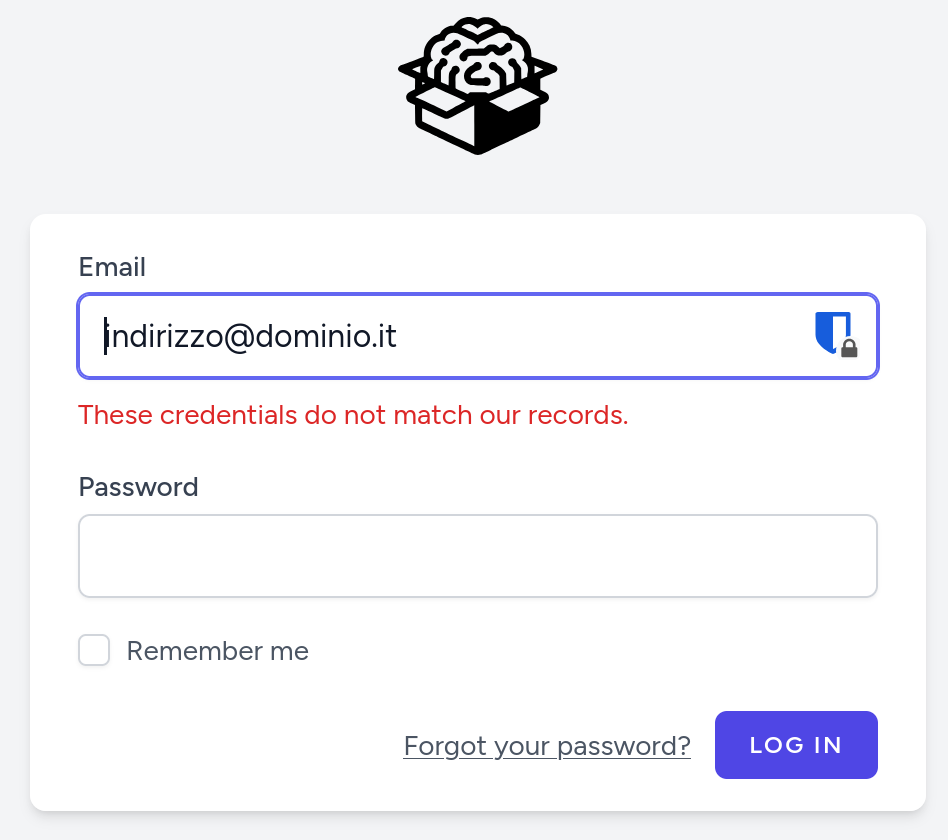
\includegraphics[width=6.5cm]{Screenshots/foglio1/Problema009.png}\hspace*{\fill}
    \vspace{10pt}
    \\
    \hline
    \textbf{Nome del valutatore} & Legati, Rinaldi, Kharef \\
    \hline
  \end{tabular}
\end{table}

% Problema \getNumeroProblema
\begin{table}[htbp]
  \centering
  \renewcommand{\arraystretch}{1.5}
  \begin{tabular}{|>{\raggedright\arraybackslash}p{7.5cm}|>{\raggedright\arraybackslash}p{7.5cm}|}
    \hline
    \rowcolor{green!30}
    \multicolumn{2}{|c|}{\textbf{Problema \getNumeroProblema}} \\
    \hline
    \textbf{Descrizione} & Dalle pagine di registrazione e di login non è possibile tornare alla homepage.\\
    \hline
    \textbf{Pagina del sito} & Registrazione e Login \\
    \hline
    \textbf{Principi violati} & 3 (Controllo dell'utente e libertà); 6 (Assicurare flessibilità ed efficienza d’uso) \\
    \hline
    \textbf{Grado di severità} & 2 (Problema secondario) \\
    \hline
    \textbf{Screen} &
    \vspace{10pt}
    \hspace*{\fill}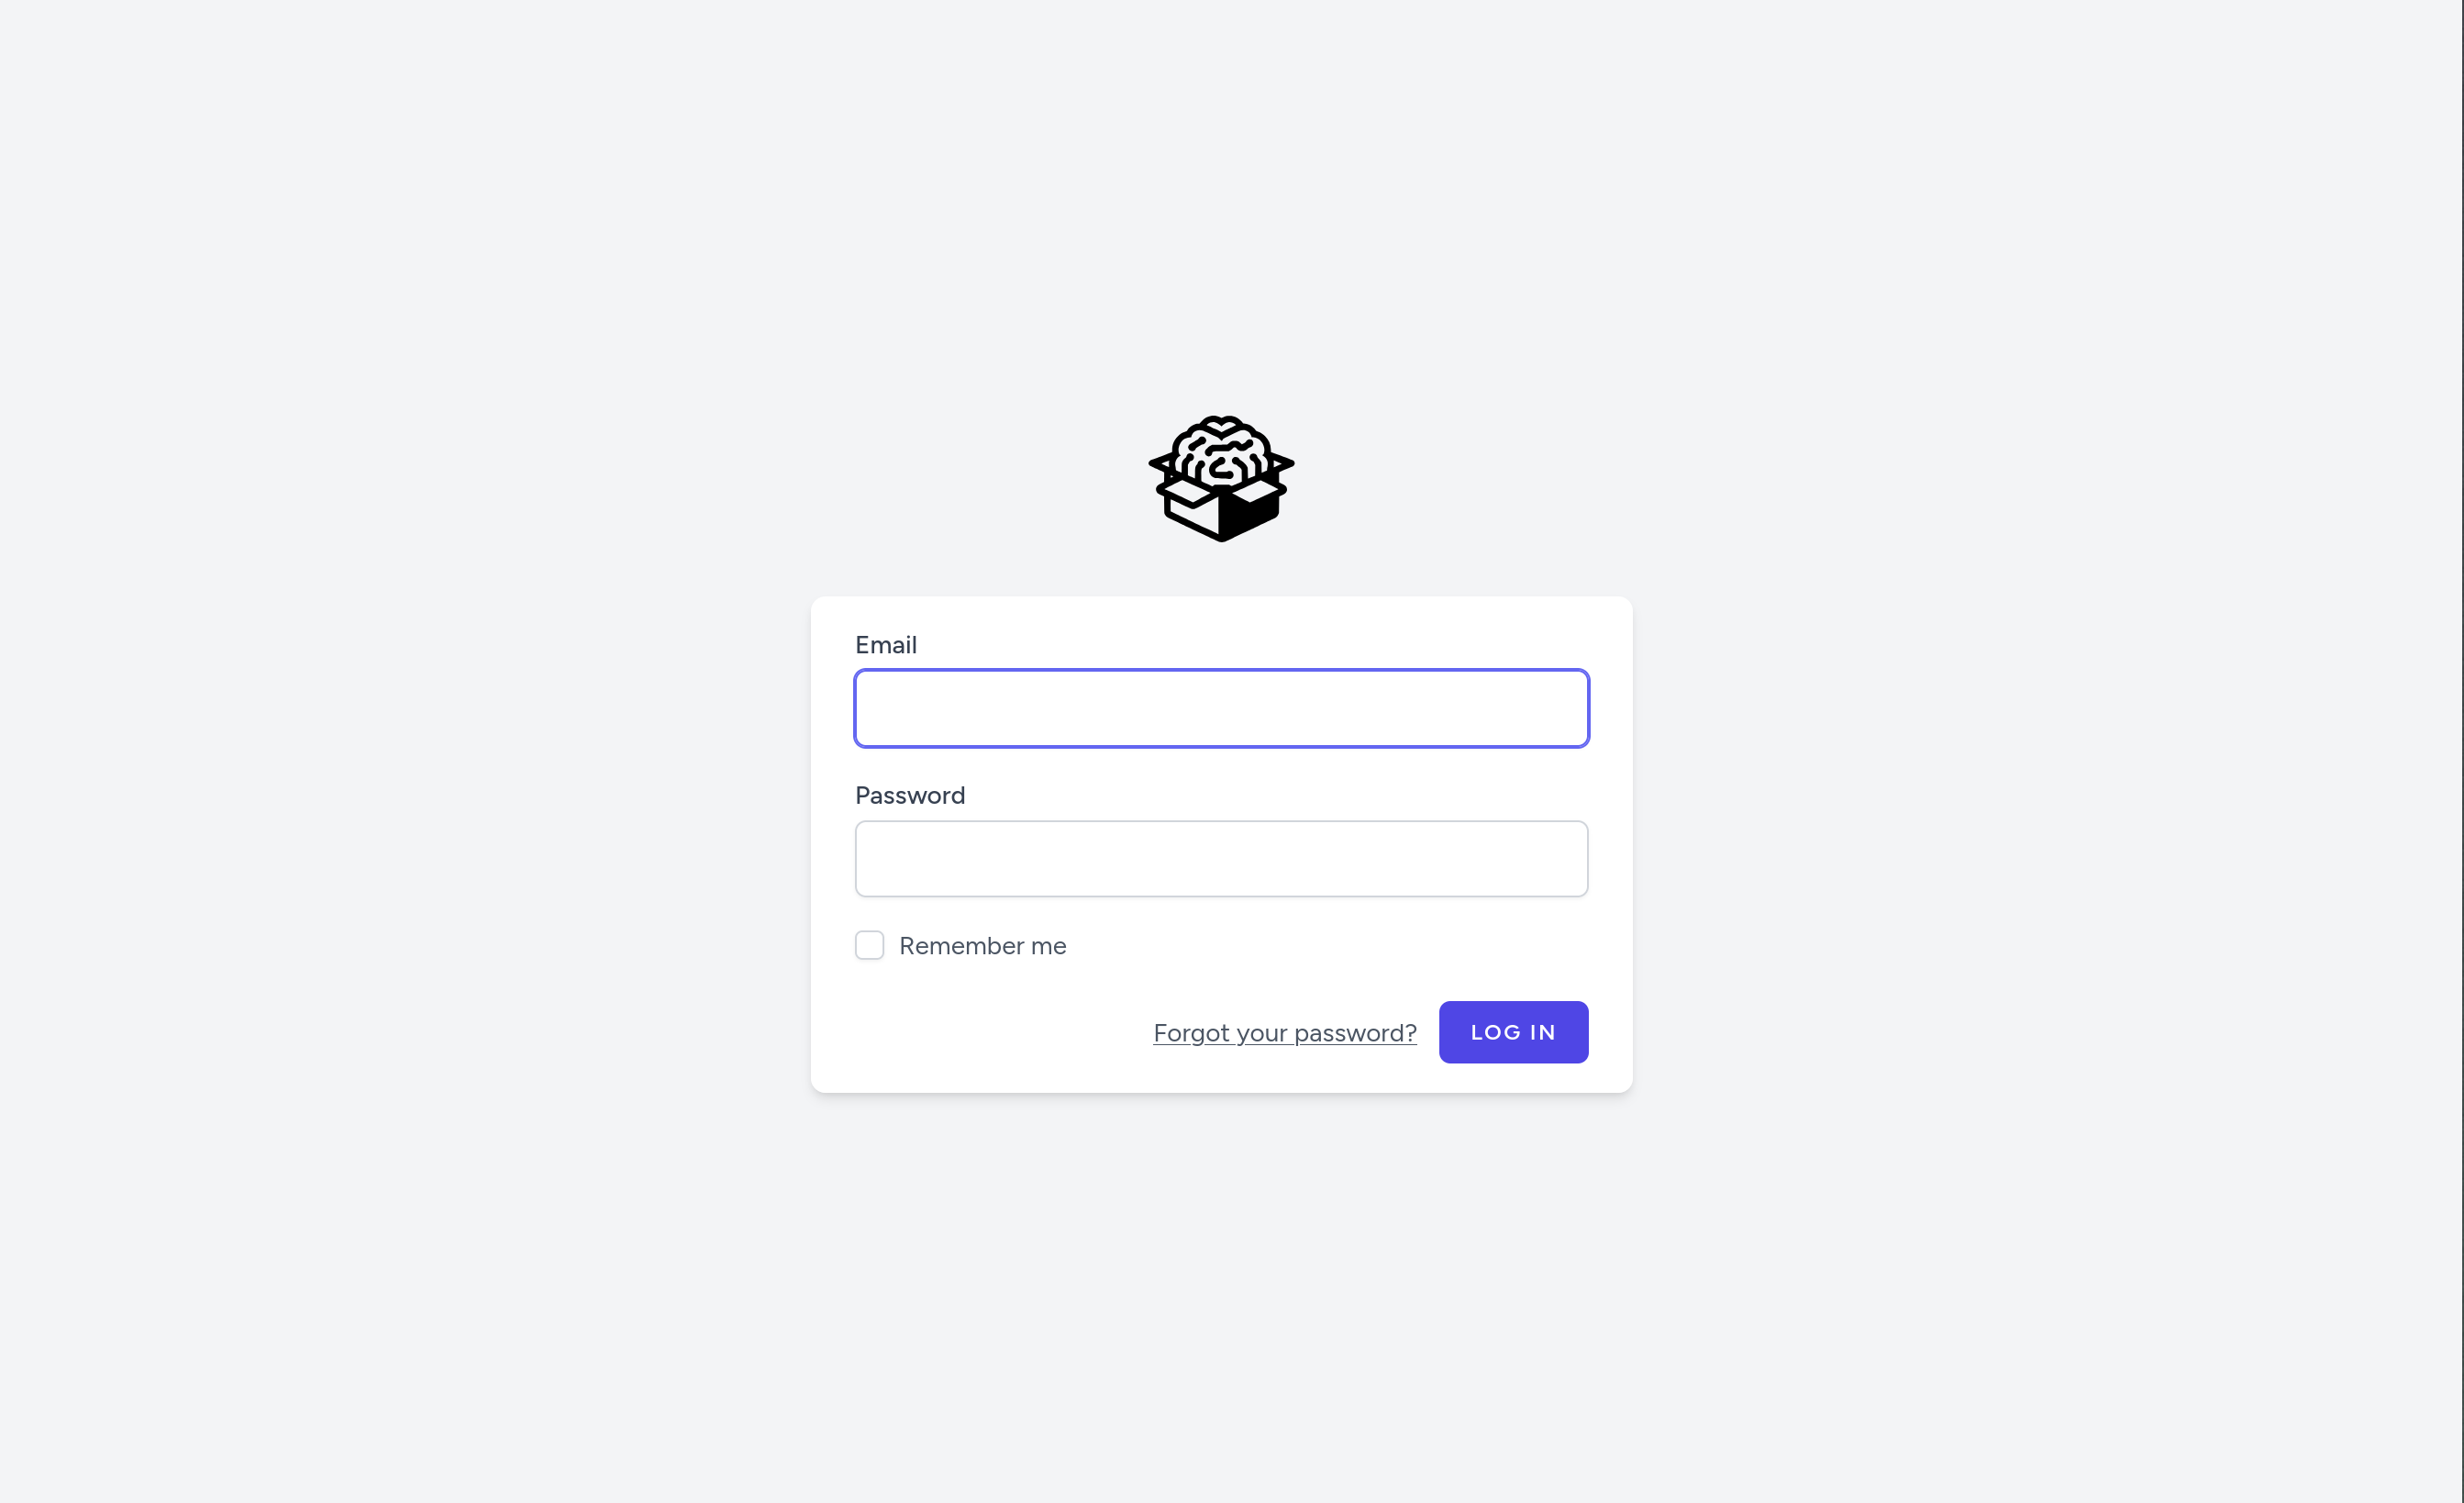
\includegraphics[width=6.5cm]{Screenshots/foglio1/Problema010.png}\hspace*{\fill}
    \vspace{10pt}
    \\
    \hline
    \textbf{Nome del valutatore} & Legati \\
    \hline
  \end{tabular}
\end{table}

% Problema \getNumeroProblema
\begin{table}[htbp]
  \centering
  \renewcommand{\arraystretch}{1.5}
  \begin{tabular}{|>{\raggedright\arraybackslash}p{7.5cm}|>{\raggedright\arraybackslash}p{7.5cm}|}
    \hline
    \rowcolor{green!30}
    \multicolumn{2}{|c|}{\textbf{Problema \getNumeroProblema}} \\
    \hline
    \textbf{Descrizione} & Nella dashboard, titoli, etichette e blocchi di testo sono un mix di italiano e inglese, compromettendo la coerenza linguistica. \\
    \hline
    \textbf{Pagina del sito} & Dashboard \\
    \hline
    \textbf{Principi violati} & 2 (Adeguare il sistema al mondo reale); 4 (Assicurare consistenza) \\
    \hline
    \textbf{Grado di severità} & 2 (Problema secondario) \\
    \hline
    \textbf{Screen} &
    \vspace{10pt}
    \hspace*{\fill}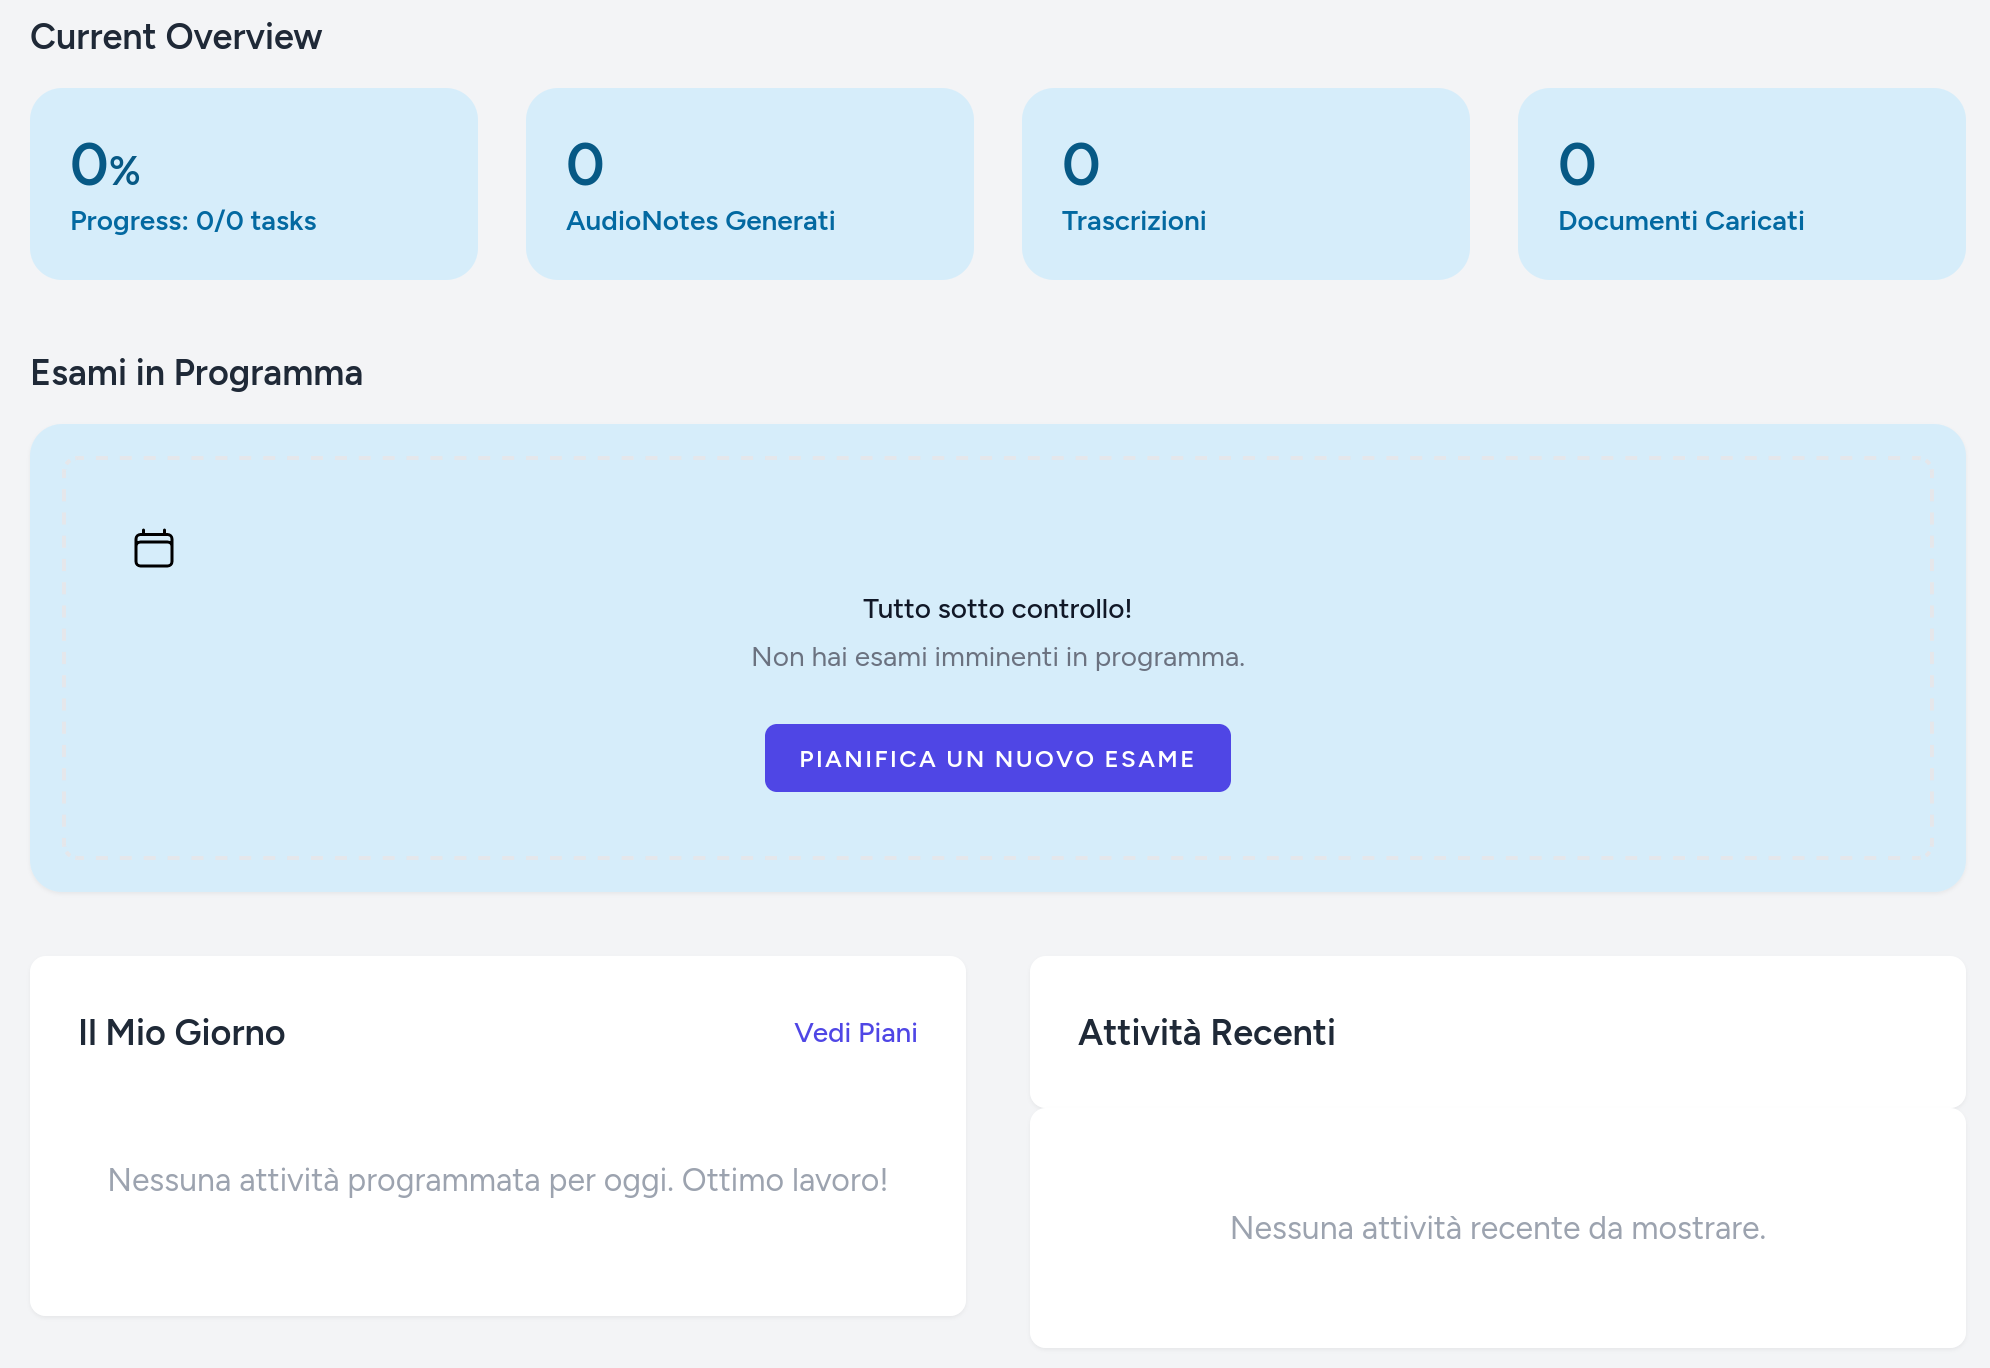
\includegraphics[width=6.5cm]{Screenshots/foglio1/Problema011.png}\hspace*{\fill}
    \vspace{10pt}
    \\
    \hline
    \textbf{Nome del valutatore} & Legati, Rinaldi, Kharef \\
    \hline
  \end{tabular}
\end{table}

% Problema \getNumeroProblema
\begin{table}[htbp]
  \centering
  \renewcommand{\arraystretch}{1.5}
  \begin{tabular}{|>{\raggedright\arraybackslash}p{7.5cm}|>{\raggedright\arraybackslash}p{7.5cm}|}
    \hline
    \rowcolor{green!30}
    \multicolumn{2}{|c|}{\textbf{Problema \getNumeroProblema}} \\
    \hline
    \textbf{Descrizione} & Il pulsante in alto a destra per le notifiche non è funzionante. \\
    \hline
    \textbf{Pagina del sito} & Dashboard \\
    \hline
    \textbf{Principi violati} & 1 (Far vedere lo stato del sistema); \\
    \hline
    \textbf{Grado di severità} & 4 (Catastrofe di usabilità) \\
    \hline
    \textbf{Screen} &
    \vspace{10pt}
    \hspace*{\fill}
\includegraphics[width=6.5cm]{Screenshots/foglio1/Problema012.png}\hspace*{\fill}
    \vspace{10pt}
    \\
    \hline
    \textbf{Nome del valutatore} & Legati, Rinaldi, Kharef \\
    \hline
  \end{tabular}
\end{table}

% Problema \getNumeroProblema
\begin{table}[htbp]
  \centering
  \renewcommand{\arraystretch}{1.5}
  \begin{tabular}{|>{\raggedright\arraybackslash}p{7.5cm}|>{\raggedright\arraybackslash}p{7.5cm}|}
    \hline
    \rowcolor{green!30}
    \multicolumn{2}{|c|}{\textbf{Problema \getNumeroProblema}} \\
    \hline
    \textbf{Descrizione} & Nelle impostazioni del profilo, il testo è scritto interamente in inglese. \\
    \hline
    \textbf{Pagina del sito} & Dashboard - Profilo \\
    \hline
    \textbf{Principi violati} & 2 (Adeguare il sistema al mondo reale) \\
    \hline
    \textbf{Grado di severità} & 2 (Problema secondario) \\
    \hline
    \textbf{Screen} &
    \vspace{10pt}
    \hspace*{\fill}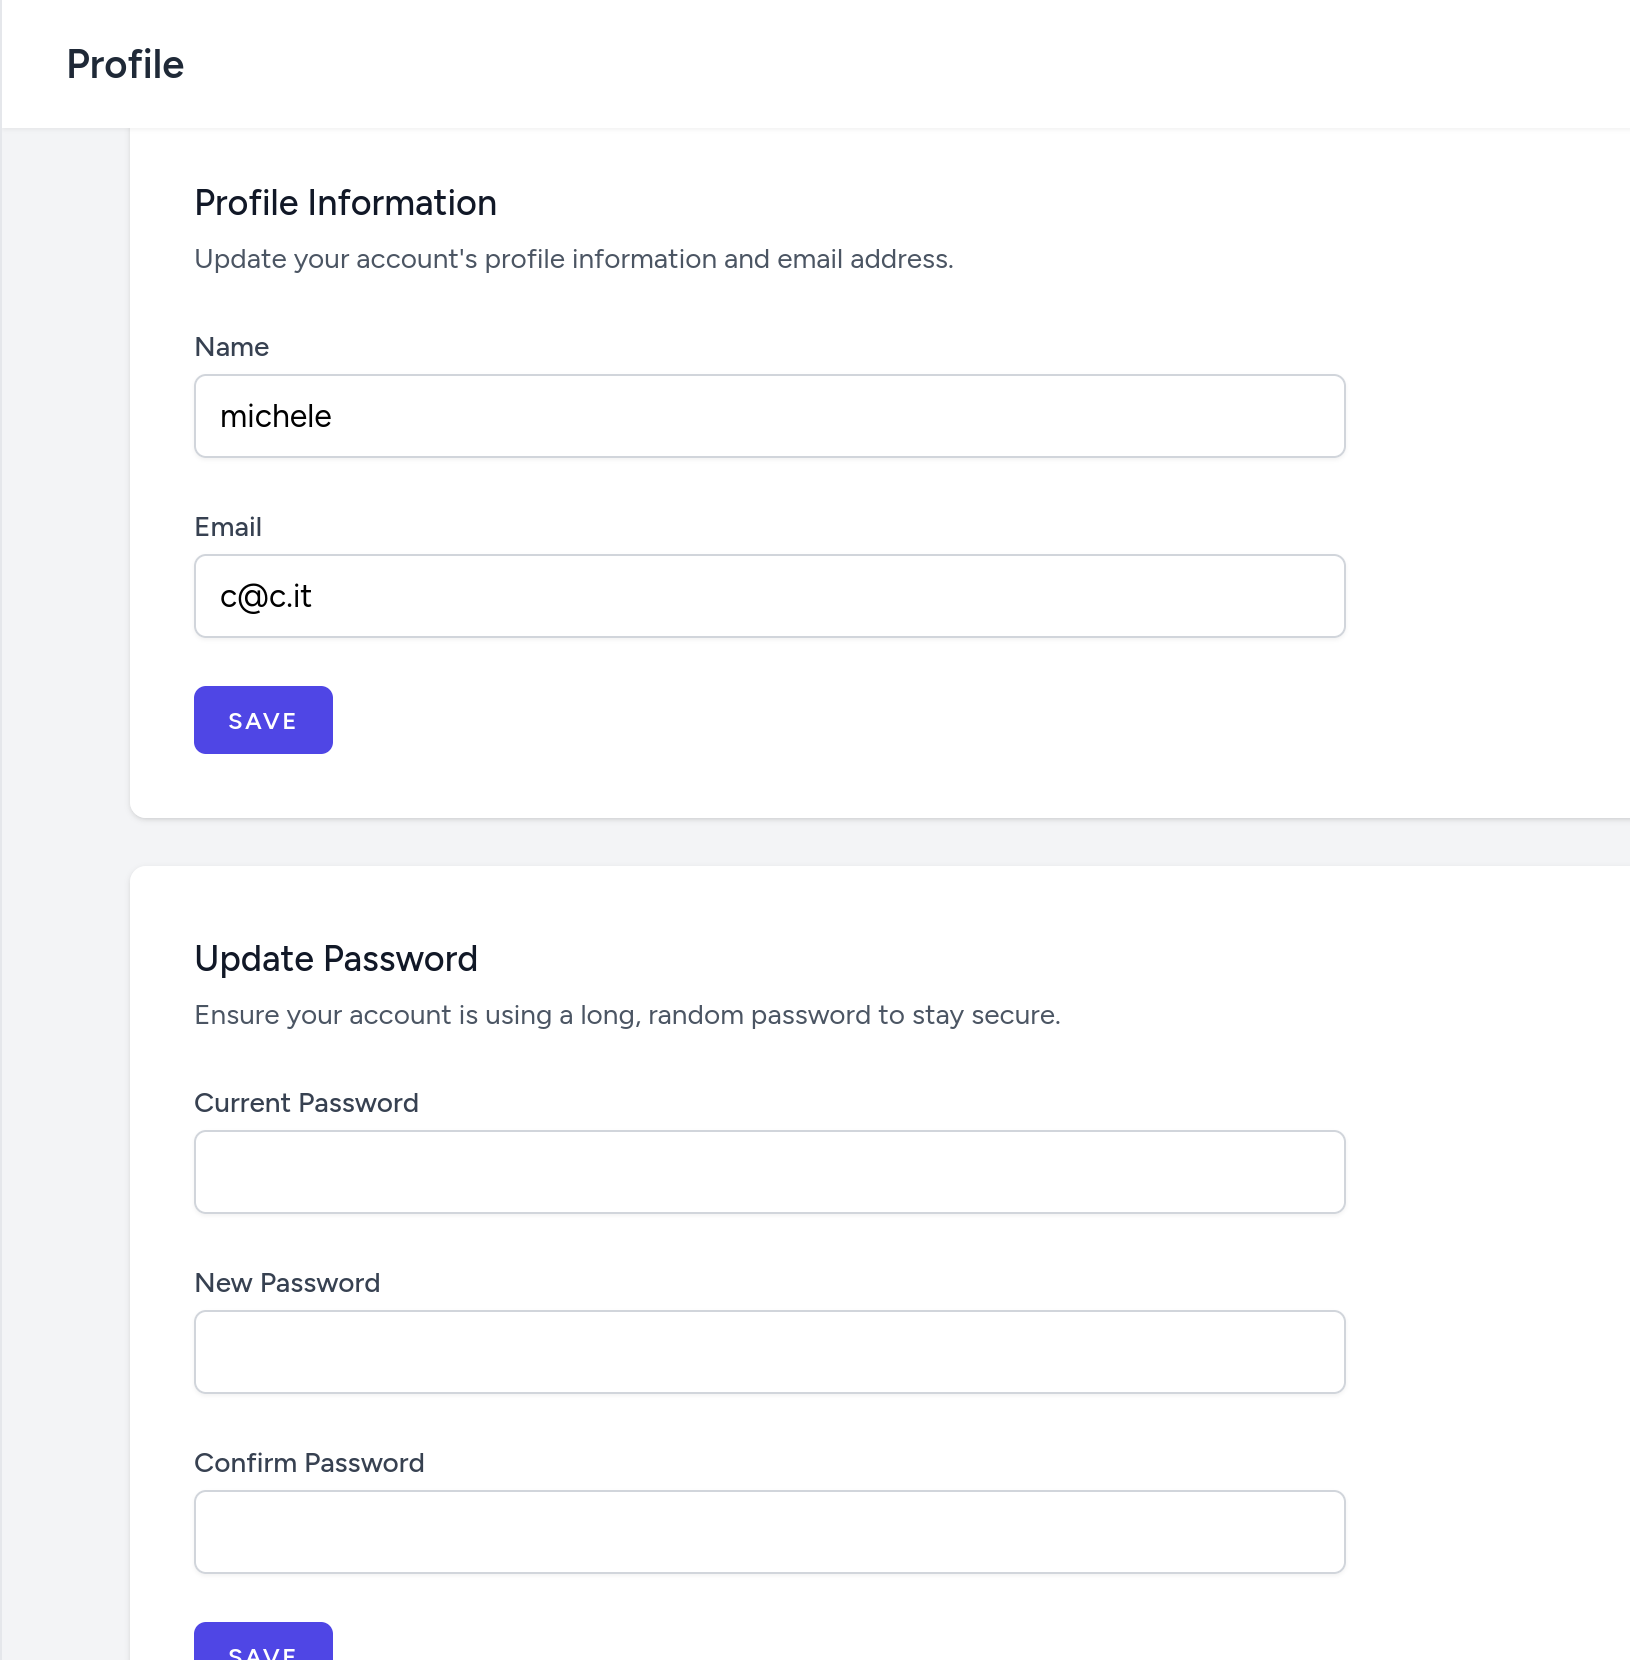
\includegraphics[width=6.5cm]{Screenshots/foglio1/Problema013.png}\hspace*{\fill}
    \vspace{10pt}
    \\
    \hline
    \textbf{Nome del valutatore} & Legati, Rinaldi \\
    \hline
  \end{tabular}
\end{table}

% Problema \getNumeroProblema
\begin{table}[htbp]
  \centering
  \renewcommand{\arraystretch}{1.5}
  \begin{tabular}{|>{\raggedright\arraybackslash}p{7.5cm}|>{\raggedright\arraybackslash}p{7.5cm}|}
    \hline
    \rowcolor{green!30}
    \multicolumn{2}{|c|}{\textbf{Problema \getNumeroProblema}} \\
    \hline
    \textbf{Descrizione} & Il pulsante di logout non chiede conferma all'utente prima di disconnettersi. \\
    \hline
    \textbf{Pagina del sito} & Dashboard - Logout \\
    \hline
    \textbf{Principi violati} & 8 (Prevenire gli errori); 9 (Permettere all'utente di correggere gli errori) \\
    \hline
    \textbf{Grado di severità} & 2 (Problema secondario) \\
    \hline
    \textbf{Screen} &
    \vspace{10pt}
    \hspace*{\fill}
\includegraphics[width=6.5cm]{Screenshots/foglio1/Problema014.png}\hspace*{\fill}
    \vspace{10pt}
    \\
    \hline
    \textbf{Nome del valutatore} & Legati, Rinaldi \\
    \hline
  \end{tabular}
\end{table}

% Problema \getNumeroProblema
\begin{table}[htbp]
  \centering
  \renewcommand{\arraystretch}{1.5}
  \begin{tabular}{|>{\raggedright\arraybackslash}p{7.5cm}|>{\raggedright\arraybackslash}p{7.5cm}|}
    \hline
    \rowcolor{green!30}
    \multicolumn{2}{|c|}{\textbf{Problema \getNumeroProblema}} \\
    \hline
    \textbf{Descrizione} & La modalità notte rende alcuni testi poco visibili, compromettendo la leggibilità. \\
    \hline
    \textbf{Pagina del sito} & Dashboard \\
    \hline
    \textbf{Principi violati} & 5 (Riconoscimento piuttosto che uso della memoria dell’utente); 7 (Visualizzare tutte e sole le informazioni necessarie) \\
    \hline
    \textbf{Grado di severità} & 2 (Problema secondario) \\
    \hline
    \textbf{Screen} &
    \vspace{10pt}
    \hspace*{\fill}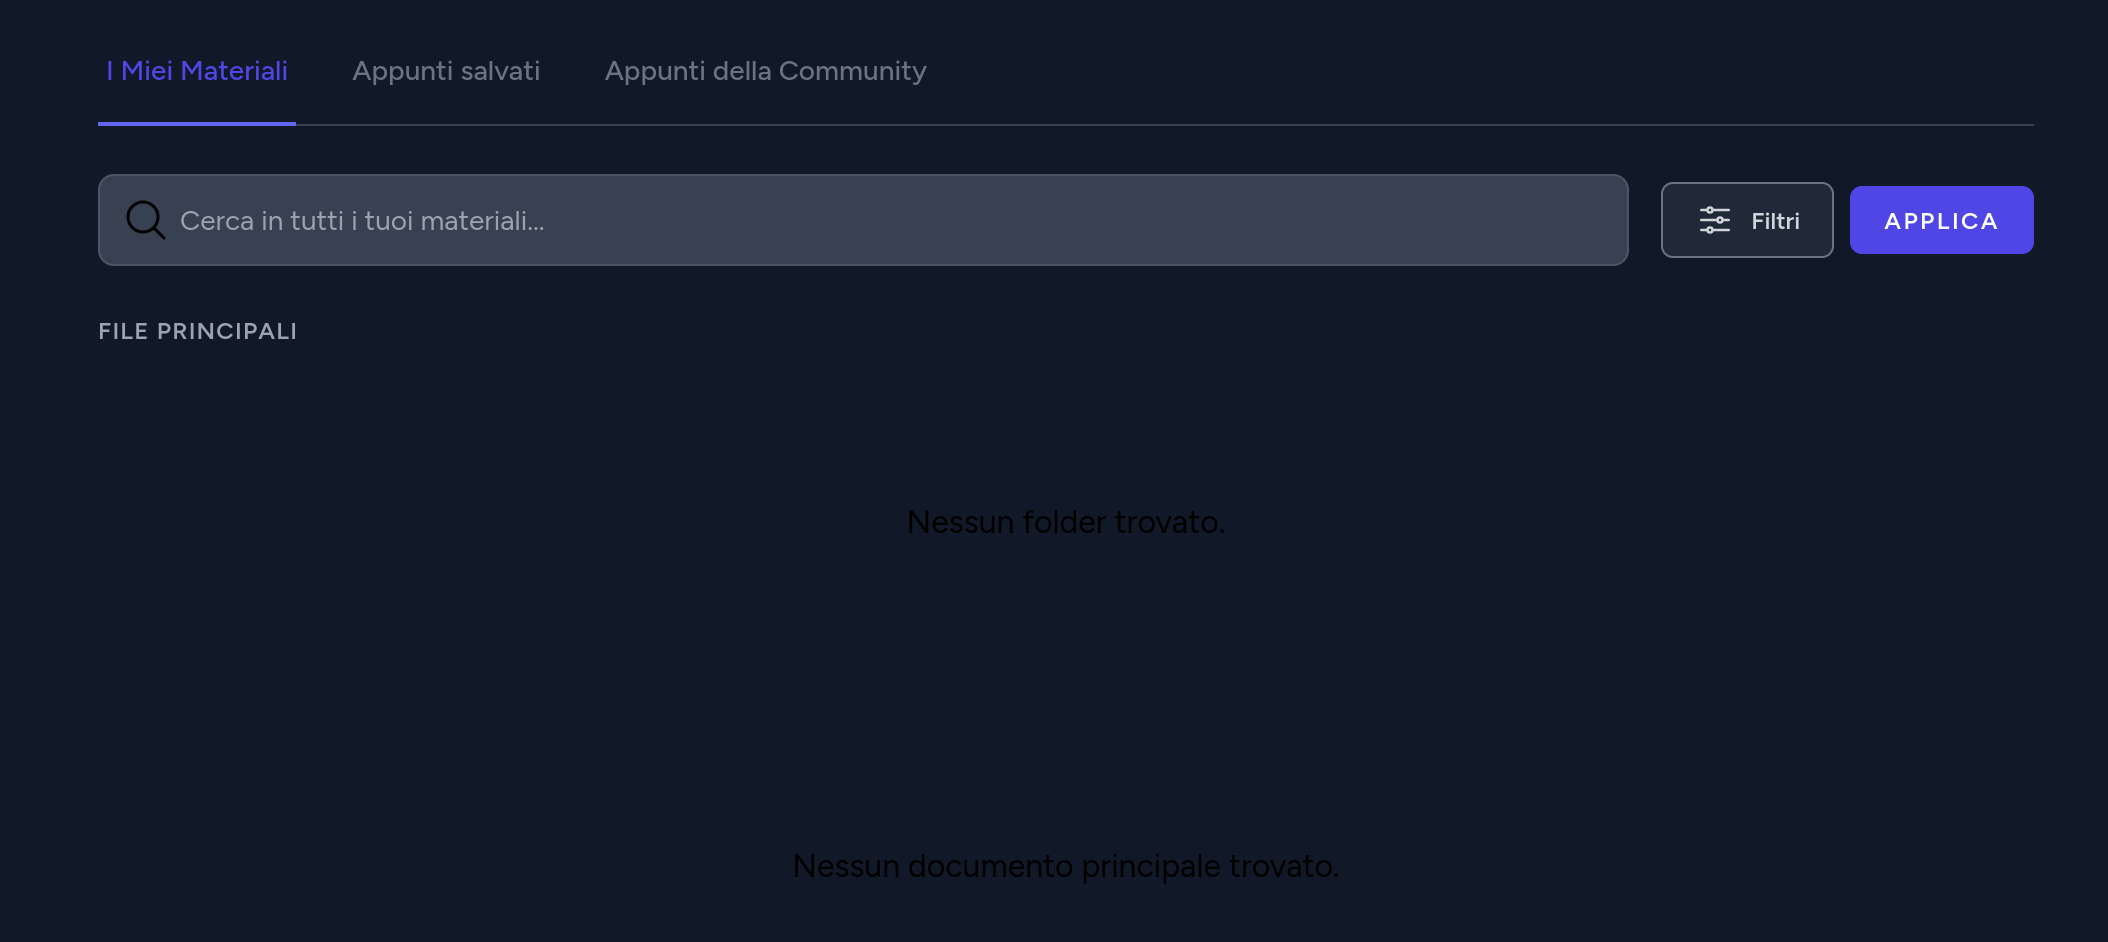
\includegraphics[width=6.5cm]{Screenshots/foglio1/Problema015.png}\hspace*{\fill}
    \vspace{10pt}
    \\
    \hline
    \textbf{Nome del valutatore} & Legati, Kharef \\
    \hline
  \end{tabular}
\end{table}

% Problema \getNumeroProblema
\begin{table}[htbp]
  \centering
  \renewcommand{\arraystretch}{1.5}
  \begin{tabular}{|>{\raggedright\arraybackslash}p{7.5cm}|>{\raggedright\arraybackslash}p{7.5cm}|}
    \hline
    \rowcolor{green!30}
    \multicolumn{2}{|c|}{\textbf{Problema \getNumeroProblema}} \\
    \hline
    \textbf{Descrizione} & In modalità notte, la selezione di qualsiasi pulsante con una funzione genera un effetto "flash" (l'interfaccia torna brevemente alla modalità chiara). \\
    \hline
    \textbf{Pagina del sito} & Dashboard \\
    \hline
    \textbf{Principi violati} & 4 (Assicurare consistenza) \\
    \hline
    \textbf{Grado di severità} & 3 (Problema rilevante) \\ \\
    \hline
    \textbf{Nome del valutatore} & Rinaldi \\
    \hline
  \end{tabular}
\end{table}

% Problema \getNumeroProblema
\begin{table}[htbp]
  \centering
  \renewcommand{\arraystretch}{1.5}
  \begin{tabular}{|>{\raggedright\arraybackslash}p{7.5cm}|>{\raggedright\arraybackslash}p{7.5cm}|}
    \hline
    \rowcolor{green!30}
    \multicolumn{2}{|c|}{\textbf{Problema \getNumeroProblema}} \\
    \hline
    \textbf{Descrizione} & Il pulsante in basso a destra "Passa a BrainBox Pro +" non è funzionante e non rimanda a nulla. \\
    \hline
    \textbf{Pagina del sito} & Dashboard \\
    \hline
    \textbf{Principi violati} & 1 (Far vedere lo stato del sistema); 5 (Riconoscimento piuttosto che uso della memoria dell’utente) \\
    \hline
    \textbf{Grado di severità} & 3 (Problema rilevante) \\
    \hline
    \textbf{Screen} &
    \vspace{10pt}
    \hspace*{\fill}
\includegraphics[width=6.5cm]{Screenshots/foglio1/Problema017.png}\hspace*{\fill}
    \vspace{10pt}
    \\
    \hline
    \textbf{Nome del valutatore} & Legati, Rinaldi, Kharef \\
    \hline
  \end{tabular}
\end{table}

% Problema \getNumeroProblema
\begin{table}[htbp]
  \centering
  \renewcommand{\arraystretch}{1.5}
  \begin{tabular}{|>{\raggedright\arraybackslash}p{7.5cm}|>{\raggedright\arraybackslash}p{7.5cm}|}
    \hline
    \rowcolor{green!30}
    \multicolumn{2}{|c|}{\textbf{Problema \getNumeroProblema}} \\
    \hline
    \textbf{Descrizione} & Nei campi password dei form di login e registrazione non è possibile visualizzare la password inserita. \\
    \hline
    \textbf{Pagina del sito} & Registrazione e Login \\
    \hline
    \textbf{Principi violati} & 1 (Far vedere lo stato del sistema); 5 (Riconoscimento piuttosto che uso della memoria dell'utente); 6 (Assicurare flessibilità ed efficienza d'uso) \\
    \hline
    \textbf{Grado di severità} & 3 (Problema rilevante) \\
    \hline
    \textbf{Screen} &
    \vspace{10pt}
    \hspace*{\fill}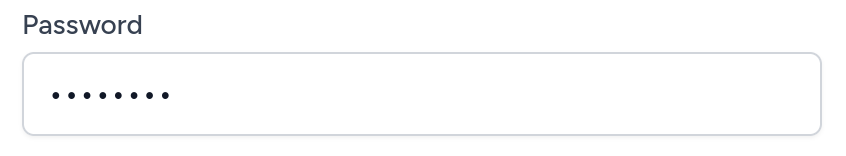
\includegraphics[width=6.5cm]{Screenshots/foglio1/Problema018.png}\hspace*{\fill}
    \vspace{10pt}
    \\
    \hline
    \textbf{Nome del valutatore} & Rinaldi \\
    \hline
  \end{tabular}
\end{table}

% Problema \getNumeroProblema
\begin{table}[htbp]
  \centering
  \renewcommand{\arraystretch}{1.5}
  \begin{tabular}{|>{\raggedright\arraybackslash}p{7.5cm}|>{\raggedright\arraybackslash}p{7.5cm}|}
    \hline
    \rowcolor{green!30}
    \multicolumn{2}{|c|}{\textbf{Problema \getNumeroProblema}} \\
    \hline
    \textbf{Descrizione} & Nella sezione "Completa il tuo profilo" (della registrazione) il menu a tendina consente di selezionare la voce "Seleziona la tua università" (che non dovrebbe essere selezionabile), analogamente a quanto avviene per i campi "Dipartimento" e "Ciclo di studi". \\
    \hline
    \textbf{Pagina del sito} & Registrazione \\
    \hline
    \textbf{Principi violati} & 7 (Visualizzare tutte e sole le informazioni necessarie); 8 (Prevenire gli errori) \\
    \hline
    \textbf{Grado di severità} & 2 (Problema secondario) \\
    \hline
    \textbf{Screen} &
    \vspace{10pt}
    \hspace*{\fill}
\includegraphics[width=6.5cm]{Screenshots/foglio1/Problema019.png}\hspace*{\fill}
    \vspace{10pt}
    \\
    \hline
    \textbf{Nome del valutatore} & Rinaldi \\
    \hline
  \end{tabular}
\end{table}

% Problema \getNumeroProblema (Basato su Legati [2])
\begin{table}[htbp]
  \centering
  \renewcommand{\arraystretch}{1.5}
  \begin{tabular}{|>{\raggedright\arraybackslash}p{7.5cm}|>{\raggedright\arraybackslash}p{7.5cm}|}
    \hline
    \rowcolor{green!30}
    \multicolumn{2}{|c|}{\textbf{Problema \getNumeroProblema}} \\
    \hline
    \textbf{Descrizione} & Nella pagina "I Miei Appunti", il titolo della pagina è scritto in inglese. \\
    \hline
    \textbf{Pagina del sito} & Dashboard - I Miei Appunti \\
    \hline
    \textbf{Principi violati} & 2 (Adeguare il sistema al mondo reale); 4 (Assicurare consistenza) \\
    \hline
    \textbf{Grado di severità} & 2 (Problema secondario) \\
    \hline
    \textbf{Screen} &
    \vspace{10pt}
    \hspace*{\fill}
\includegraphics[width=6.5cm]{Screenshots/foglio1/Problema021.png}\hspace*{\fill}
    \vspace{10pt}
    \\
    \hline
    \textbf{Nome del valutatore} & Legati, Rinaldi, Kharef \\
    \hline
  \end{tabular}
\end{table}

% Problema \getNumeroProblema (Basato su Legati [2])
\begin{table}[htbp]
  \centering
  \renewcommand{\arraystretch}{1.5}
  \begin{tabular}{|>{\raggedright\arraybackslash}p{7.5cm}|>{\raggedright\arraybackslash}p{7.5cm}|}
    \hline
    \rowcolor{green!30}
    \multicolumn{2}{|c|}{\textbf{Problema \getNumeroProblema}} \\
    \hline
    \textbf{Descrizione} & Nella pagina "I Miei Appunti", i pulsanti "CARICA FILE" e "Nuova Cartella" sono posizionati in un punto poco coerente con il contenuto della pagina. \\
    \hline
    \textbf{Pagina del sito} & Dashboard - I Miei Appunti \\
    \hline
    \textbf{Principi violati} & 5 (Riconoscimento piuttosto che uso della memoria dell’utente) \\
    \hline
    \textbf{Grado di severità} & 1 (Problema accessorio) \\
    \hline
    \textbf{Screen} &
    \vspace{10pt}
    \hspace*{\fill}
\includegraphics[width=6.5cm]{Screenshots/foglio1/Problema022.png}\hspace*{\fill}
    \vspace{10pt}
    \\
    \hline
    \textbf{Nome del valutatore} & Legati \\
    \hline
  \end{tabular}
\end{table}

% Problema \getNumeroProblema (Basato su Legati [2])
\begin{table}[htbp]
  \centering
  \renewcommand{\arraystretch}{1.5}
  \begin{tabular}{|>{\raggedright\arraybackslash}p{7.5cm}|>{\raggedright\arraybackslash}p{7.5cm}|}
    \hline
    \rowcolor{green!30}
    \multicolumn{2}{|c|}{\textbf{Problema \getNumeroProblema}} \\
    \hline
    \textbf{Descrizione} & Nella pagina "I Miei Appunti", il pulsante "CARICA FILE" è scritto in maiuscolo a differenza di tutti gli altri pulsanti. \\
    \hline
    \textbf{Pagina del sito} & Dashboard - I Miei Appunti \\
    \hline
    \textbf{Principi violati} & 4 (Assicurare consistenza) \\
    \hline
    \textbf{Grado di severità} & 1 (Problema accessorio) \\
    \hline
    \textbf{Screen} &
    \vspace{10pt}
    \hspace*{\fill}
\includegraphics[width=6.5cm]{Screenshots/foglio1/Problema023.png}\hspace*{\fill}
    \vspace{10pt}
    \\
    \hline
    \textbf{Nome del valutatore} & Legati \\
    \hline
  \end{tabular}
\end{table}

% Problema \getNumeroProblema (Basato su Legati [2])
\begin{table}[htbp]
  \centering
  \renewcommand{\arraystretch}{1.5}
  \begin{tabular}{|>{\raggedright\arraybackslash}p{7.5cm}|>{\raggedright\arraybackslash}p{7.5cm}|}
    \hline
    \rowcolor{green!30}
    \multicolumn{2}{|c|}{\textbf{Problema \getNumeroProblema}} \\
    \hline
    \textbf{Descrizione} & Nella pagina "I Miei Appunti", il pulsante "CARICA FILE" ha un'icona che non rispecchia il comportamento del pulsante. \\
    \hline
    \textbf{Pagina del sito} & Dashboard - I Miei Appunti \\
    \hline
    \textbf{Principi violati} & 2 (Adeguare il sistema al mondo reale); 5 (Riconoscimento piuttosto che uso della memoria dell’utente) \\
    \hline
    \textbf{Grado di severità} & 2 (Problema secondario) \\
    \hline
    \textbf{Screen} &
    \vspace{10pt}
    \hspace*{\fill}
\includegraphics[width=6.5cm]{Screenshots/foglio1/Problema024.png}\hspace*{\fill}
    \vspace{10pt}
    \\
    \hline
    \textbf{Nome del valutatore} & Legati \\
    \hline
  \end{tabular}
\end{table}

% Problema \getNumeroProblema (Basato su Legati [4])
\begin{table}[htbp]
  \centering
  \renewcommand{\arraystretch}{1.5}
  \begin{tabular}{|>{\raggedright\arraybackslash}p{7.5cm}|>{\raggedright\arraybackslash}p{7.5cm}|}
    \hline
    \rowcolor{green!30}
    \multicolumn{2}{|c|}{\textbf{Problema \getNumeroProblema}} \\
    \hline
    \textbf{Descrizione} & Nella pagina "I Miei Appunti", il tab "I Miei Materiali" ha un titolo poco fuorviante per la pagina; dovrebbe essere "I Miei Appunti". \\
    \hline
    \textbf{Pagina del sito} & Dashboard - I Miei Appunti \\
    \hline
    \textbf{Principi violati} & 2 (Adeguare il sistema al mondo reale); 5 (Riconoscimento piuttosto che uso della memoria dell’utente) \\
    \hline
    \textbf{Grado di severità} & 1 (Problema accessorio) \\
    \hline
    \textbf{Screen} &
    \vspace{10pt}
    \hspace*{\fill}
\includegraphics[width=6.5cm]{Screenshots/foglio1/Problema025.png}\hspace*{\fill}
    \vspace{10pt}
    \\
    \hline
    \textbf{Nome del valutatore} & Legati \\
    \hline
  \end{tabular}
\end{table}

% Problema \getNumeroProblema (Basato su Legati [4])
\begin{table}[htbp]
  \centering
  \renewcommand{\arraystretch}{1.5}
  \begin{tabular}{|>{\raggedright\arraybackslash}p{7.5cm}|>{\raggedright\arraybackslash}p{7.5cm}|}
    \hline
    \rowcolor{green!30}
    \multicolumn{2}{|c|}{\textbf{Problema \getNumeroProblema}} \\
    \hline
    \textbf{Descrizione} & Nella pagina "I Miei Appunti", una volta cliccato sul tab "Appunti Salvati" o "Appunti della Community", non è più possibile tornare indietro. Manca un pulsante o un percorso di navigazione che consenta di tornare alla pagina precedente. \\
    \hline
    \textbf{Pagina del sito} & Dashboard - I Miei Appunti \\
    \hline
    \textbf{Principi violati} & 3 (Controllo dell'utente e libertà); 6 (Assicurare flessibilità ed efficienza d’uso) \\
    \hline
    \textbf{Grado di severità} & 2 (Problema secondario) \\
    \hline
    \textbf{Screen} &
    \vspace{10pt}
    \hspace*{\fill}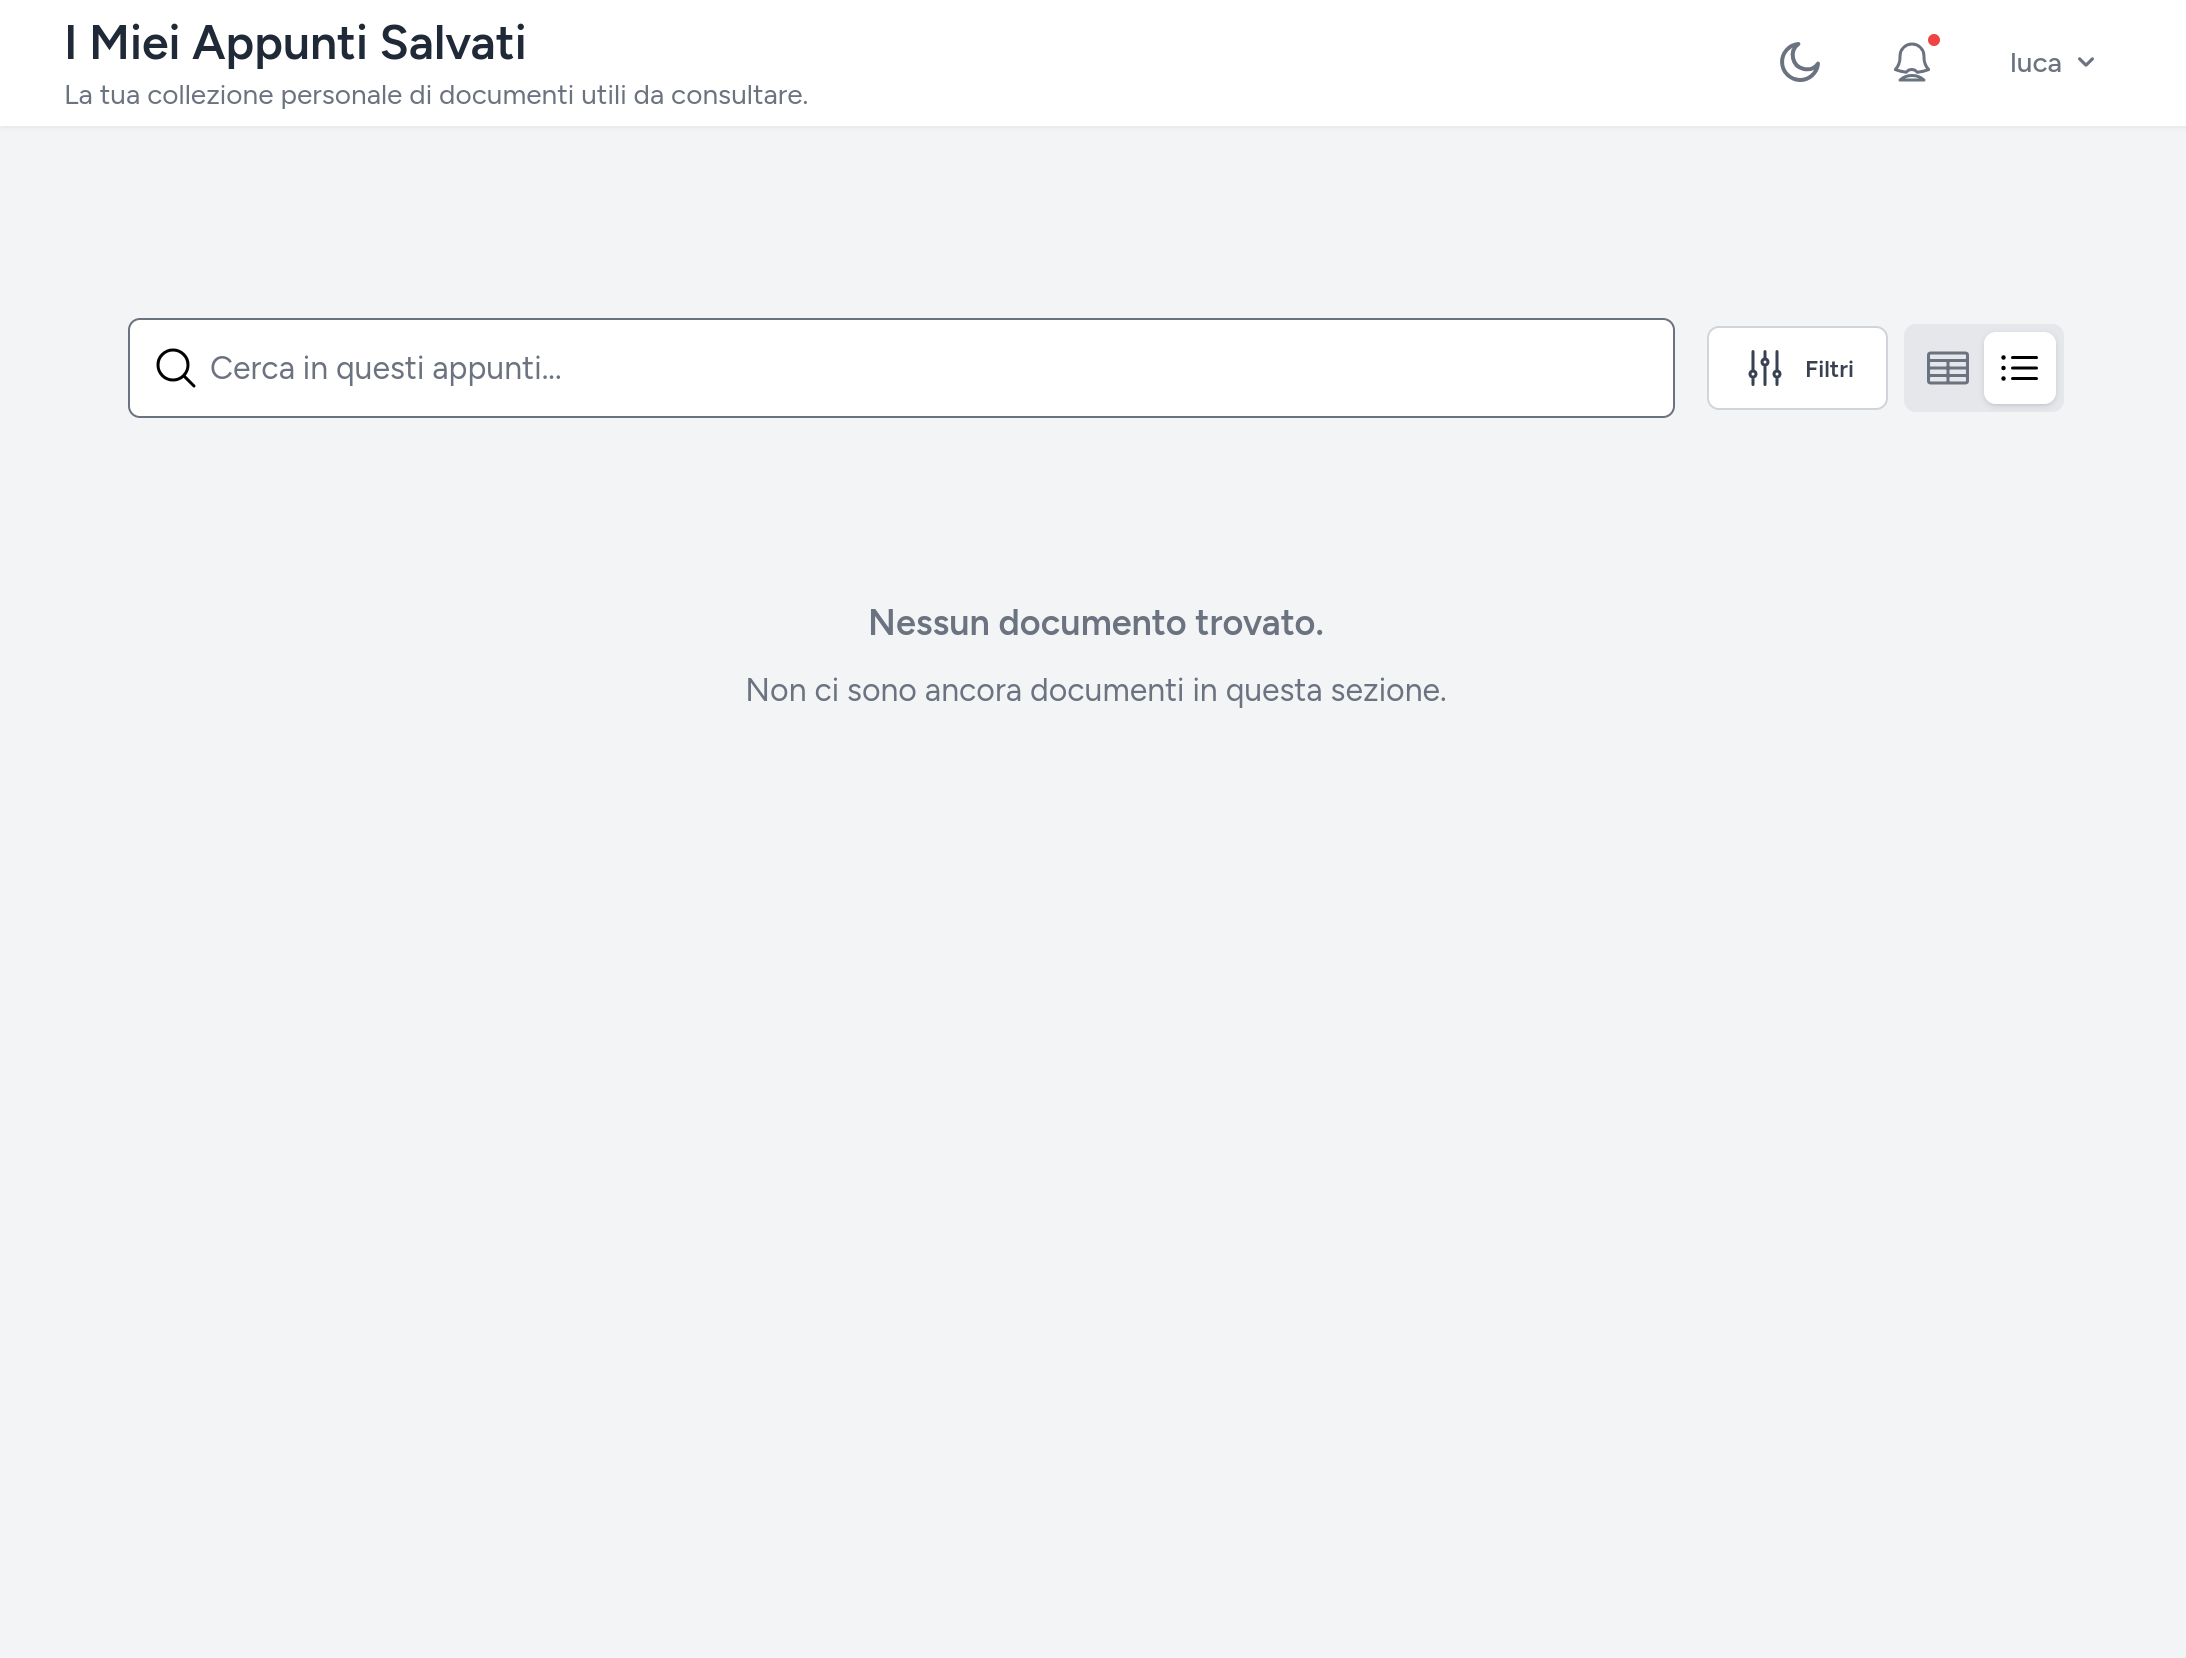
\includegraphics[width=6.5cm]{Screenshots/foglio1/Problema026.png}\hspace*{\fill}
    \vspace{10pt}
    \\
    \hline
    \textbf{Nome del valutatore} & Legati, Rinaldi \\
    \hline
  \end{tabular}
\end{table}
\FloatBarrier

% Problema \getNumeroProblema
\begin{table}[htbp]
  \centering
  \renewcommand{\arraystretch}{1.5}
  \begin{tabular}{|>{\raggedright\arraybackslash}p{7.5cm}|>{\raggedright\arraybackslash}p{7.5cm}|}
    \hline
    \rowcolor{green!30}
    \multicolumn{2}{|c|}{\textbf{Problema \getNumeroProblema}} \\
    \hline
    \textbf{Descrizione} & Nella pagina "I Miei Appunti", una volta cliccato sul tab "Appunti Salvati", viene presentata una pagina completamente diversa da quella che mi aspetterei. Analogamente cliccando sul tab "Appunti della Community". \\
    \hline
    \textbf{Pagina del sito} & Dashboard - I Miei Appunti \\
    \hline
    \textbf{Principi violati} & 2 (Adeguare il sistema al mondo reale); 4 (Assicurare consistenza) \\
    \hline
    \textbf{Grado di severità} & 2 (Problema secondario) \\
    \hline
    \textbf{Nome del valutatore} & Legati \\
    \hline
  \end{tabular}
\end{table}

% Problema \getNumeroProblema
\begin{table}[htbp]
  \centering
  \renewcommand{\arraystretch}{1.5}
  \begin{tabular}{|>{\raggedright\arraybackslash}p{7.5cm}|>{\raggedright\arraybackslash}p{7.5cm}|}
    \hline
    \rowcolor{green!30}
    \multicolumn{2}{|c|}{\textbf{Problema \getNumeroProblema}} \\
    \hline
    \textbf{Descrizione} & Durante il caricamento di un nuovo file nella sezione appunti, il titolo "Upload" è in inglese. \\
    \hline
    \textbf{Pagina del sito} & Dashboard - I Miei Appunti - Caricamento File \\
    \hline
    \textbf{Principi violati} & 2 (Adeguare il sistema al mondo reale); 4 (Assicurare consistenza) \\
    \hline
    \textbf{Grado di severità} & 2 (Problema secondario) \\
    \hline
    \textbf{Screen} &
    \vspace{10pt}
    \hspace*{\fill}
\includegraphics[width=6.5cm]{Screenshots/foglio2/problema003.png}\hspace*{\fill}
    \vspace{10pt}
    \\
    \hline
    \textbf{Nome del valutatore} & Legati, Rinaldi, Kharef \\
    \hline
  \end{tabular}
\end{table}

% Problema \getNumeroProblema
\begin{table}[htbp]
  \centering
  \renewcommand{\arraystretch}{1.5}
  \begin{tabular}{|>{\raggedright\arraybackslash}p{7.5cm}|>{\raggedright\arraybackslash}p{7.5cm}|}
    \hline
    \rowcolor{green!30}
    \multicolumn{2}{|c|}{\textbf{Problema \getNumeroProblema}} \\
    \hline
    \textbf{Descrizione} & Durante il caricamento di un nuovo file nella sezione appunti, il titolo "Fatto" è un po' generico. \\
    \hline
    \textbf{Pagina del sito} & Dashboard - I Miei Appunti - Caricamento File \\
    \hline
    \textbf{Principi violati} & 2 (Adeguare il sistema al mondo reale); 5 (Riconoscimento piuttosto che uso della memoria dell’utente) \\
    \hline
    \textbf{Grado di severità} & 0 (Non è un problema di usabilità) \\
    \hline
    \textbf{Screen} &
    \vspace{10pt}
    \hspace*{\fill}
\includegraphics[width=6.5cm]{Screenshots/foglio2/problema004.png}\hspace*{\fill}
    \vspace{10pt}
    \\
    \hline
    \textbf{Nome del valutatore} & Legati \\
    \hline
  \end{tabular}
\end{table}

% Problema \getNumeroProblema
\begin{table}[htbp]
  \centering
  \renewcommand{\arraystretch}{1.5}
  \begin{tabular}{|>{\raggedright\arraybackslash}p{7.5cm}|>{\raggedright\arraybackslash}p{7.5cm}|}
    \hline
    \rowcolor{green!30}
    \multicolumn{2}{|c|}{\textbf{Problema \getNumeroProblema}} \\
    \hline
    \textbf{Descrizione} & Durante il caricamento di un nuovo file nella sezione appunti, la modifica dei valori nella sezione "Dettagli" implica un refresh visibile del contenuto. \\
    \hline
    \textbf{Pagina del sito} & Dashboard - I Miei Appunti - Caricamento File \\
    \hline
    \textbf{Principi violati} & 4 (Assicurare consistenza) \\
    \hline
    \textbf{Grado di severità} & 3 (Problema rilevante) \\
    \hline
    \textbf{Nome del valutatore} & Legati, Kharef \\
    \hline
  \end{tabular}
\end{table}

% Problema \getNumeroProblema
\begin{table}[htbp]
  \centering
  \renewcommand{\arraystretch}{1.5}
  \begin{tabular}{|>{\raggedright\arraybackslash}p{7.5cm}|>{\raggedright\arraybackslash}p{7.5cm}|}
    \hline
    \rowcolor{green!30}
    \multicolumn{2}{|c|}{\textbf{Problema \getNumeroProblema}} \\
    \hline
    \textbf{Descrizione} & Durante il caricamento di un nuovo file nella sezione appunti, i messaggi di errore nella sezione "Dettagli" sono scritti in inglese. \\
    \hline
    \textbf{Pagina del sito} & Dashboard - I Miei Appunti - Caricamento File \\
    \hline
    \textbf{Principi violati} & 2 (Adeguare il sistema al mondo reale); 4 (Assicurare consistenza); 9 (Permettere all’utente di correggere gli errori e non solo di rilevarli) \\
    \hline
    \textbf{Grado di severità} & 2 (Problema secondario) \\
    \hline
    \textbf{Screen} &
    \vspace{10pt}
    \hspace*{\fill}
\includegraphics[width=6.5cm]{Screenshots/foglio2/problema006.png}\hspace*{\fill}
    \vspace{10pt}
    \\
    \hline
    \textbf{Nome del valutatore} & Legati, Rinaldi \\
    \hline
  \end{tabular}
\end{table}

% Problema \getNumeroProblema
\begin{table}[htbp]
  \centering
  \renewcommand{\arraystretch}{1.5}
  \begin{tabular}{|>{\raggedright\arraybackslash}p{7.5cm}|>{\raggedright\arraybackslash}p{7.5cm}|}
    \hline
    \rowcolor{green!30}
    \multicolumn{2}{|c|}{\textbf{Problema \getNumeroProblema}} \\
    \hline
    \textbf{Descrizione} & Durante il caricamento di un nuovo file nella sezione appunti, i messaggi di errore nella sezione "Dettagli" non scompaiono dopo che il contenuto del campo è stato modificato (e validato). \\
    \hline
    \textbf{Pagina del sito} & Dashboard - I Miei Appunti - Caricamento File \\
    \hline
    \textbf{Principi violati} & 1 (Far vedere lo stato del sistema); 8 (Prevenire gli errori) \\
    \hline
    \textbf{Grado di severità} & 3 (Problema rilevante) \\
    \hline
    \textbf{Screen} &
    \vspace{10pt}
    \hspace*{\fill}
\includegraphics[width=6.5cm]{Screenshots/foglio2/problema007.png}\hspace*{\fill}
    \vspace{10pt}
    \\
    \hline
    \textbf{Nome del valutatore} & Legati \\
    \hline
  \end{tabular}
\end{table}

% Problema \getNumeroProblema
\begin{table}[htbp]
  \centering
  \renewcommand{\arraystretch}{1.5}
  \begin{tabular}{|>{\raggedright\arraybackslash}p{7.5cm}|>{\raggedright\arraybackslash}p{7.5cm}|}
    \hline
    \rowcolor{green!30}
    \multicolumn{2}{|c|}{\textbf{Problema \getNumeroProblema}} \\
    \hline
    \textbf{Descrizione} & Nella pagina "I Miei Appunti" e "I Miei Materiali", se non sono presenti cartelle e file compare il messaggio "no folder trovato", un mix di italiano e inglese. \\
    \hline
    \textbf{Pagina del sito} & Dashboard - I Miei Appunti - I Miei Materiali \\
    \hline
    \textbf{Principi violati} & 2 (Adeguare il sistema al mondo reale); 4 (Assicurare consistenza) \\
    \hline
    \textbf{Grado di severità} & 2 (Problema secondario) \\
    \hline
    \textbf{Screen} &
    \vspace{10pt}
    \hspace*{\fill}
\includegraphics[width=6.5cm]{Screenshots/foglio2/problema008.png}\hspace*{\fill}
    \vspace{10pt}
    \\
    \hline
    \textbf{Nome del valutatore} & Legati, Rinaldi \\
    \hline
  \end{tabular}
\end{table}

% Problema \getNumeroProblema
\begin{table}[htbp]
  \centering
  \renewcommand{\arraystretch}{1.5}
  \begin{tabular}{|>{\raggedright\arraybackslash}p{7.5cm}|>{\raggedright\arraybackslash}p{7.5cm}|}
    \hline
    \rowcolor{green!30}
    \multicolumn{2}{|c|}{\textbf{Problema \getNumeroProblema}} \\
    \hline
    \textbf{Descrizione} & Nella pagina "Mostra Documento", la sezione "Caricato da" (l'autore) non è cliccabile. \\
    \hline
    \textbf{Pagina del sito} & Dashboard - I Miei Appunti - Mostra Documento \\
    \hline
    \textbf{Principi violati} & 5 (Riconoscimento piuttosto che uso della memoria dell’utente); 6 (Assicurare flessibilità ed efficienza d’uso) \\
    \hline
    \textbf{Grado di severità} & 2 (Problema secondario) \\
    \hline
    \textbf{Nome del valutatore} & Legati, Kharef \\
    \hline
  \end{tabular}
\end{table}

% Problema \getNumeroProblema
\begin{table}[htbp]
  \centering
  \renewcommand{\arraystretch}{1.5}
  \begin{tabular}{|>{\raggedright\arraybackslash}p{7.5cm}|>{\raggedright\arraybackslash}p{7.5cm}|}
    \hline
    \rowcolor{green!30}
    \multicolumn{2}{|c|}{\textbf{Problema \getNumeroProblema}} \\
    \hline
    \textbf{Descrizione} & Nella pagina "Mostra Documento" e sotto la voce "Corso", la voce non è cliccabile. \\
    \hline
    \textbf{Pagina del sito} & Dashboard - I Miei Appunti - Mostra Documento \\
    \hline
    \textbf{Principi violati} & 5 (Riconoscimento piuttosto che uso della memoria dell’utente); 6 (Assicurare flessibilità ed efficienza d’uso) \\
    \hline
    \textbf{Grado di severità} & 2 (Problema secondario) \\
    \hline
    \textbf{Nome del valutatore} & Legati \\
    \hline
  \end{tabular}
\end{table}

%----------------------------------------------------------------
\FloatBarrier

% Problema \getNumeroProblema
\begin{table}[htbp]
  \centering
  \renewcommand{\arraystretch}{1.5}
  \begin{tabular}{|>{\raggedright\arraybackslash}p{7.5cm}|>{\raggedright\arraybackslash}p{7.5cm}|}
    \hline
    \rowcolor{green!30}
    \multicolumn{2}{|c|}{\textbf{Problema \getNumeroProblema}} \\
    \hline
    \textbf{Descrizione} & Nella pagina ”Mostra Documento” e ”Commenti”, i commenti vengono visualizzati in un punto poco visibile. \\
    \hline
    \textbf{Pagina del sito} & Dashboard - I Miei Appunti - Mostra Documento \\
    \hline
    \textbf{Principi violati} & 5 (Riconoscimento piuttosto che uso della memoria dell’utente); 7 (Visualizzare tutte e sole le informazioni necessarie) \\
    \hline
    \textbf{Grado di severità} & 2 (Problema secondario) \\
    \hline
    \textbf{Nome del valutatore} & Legati, Kharef \\
    \hline
  \end{tabular}
\end{table}

% Problema \getNumeroProblema
\begin{table}[htbp]
  \centering
  \renewcommand{\arraystretch}{1.5}
  \begin{tabular}{|>{\raggedright\arraybackslash}p{7.5cm}|>{\raggedright\arraybackslash}p{7.5cm}|}
    \hline
    \rowcolor{green!30}
    \multicolumn{2}{|c|}{\textbf{Problema \getNumeroProblema}} \\
    \hline
    \textbf{Descrizione} & Nella pagina ”Esplora Appunti” e visualizzando gli appunti in una griglia, quando l'utente clicca sull'icona del documento, l'azione non funziona; è necessario cliccare il bordo della card per accedere. \\
    \hline
    \textbf{Pagina del sito} & Dashboard - Esplora Appunti \\
    \hline
    \textbf{Principi violati} & 5 (Riconoscimento piuttosto che uso della memoria dell’utente) \\
    \hline
    \textbf{Grado di severità} & 3 (Problema rilevante) \\
    \hline
    \textbf{Screen} &
    \vspace{10pt}
    \hspace*{\fill}
\includegraphics[width=6.5cm]{Screenshots/foglio3/problema63.png}\hspace*{\fill}
    \vspace{10pt}
    \\
    \hline
    \textbf{Nome del valutatore} & Legati, Kharef \\
    \hline
  \end{tabular}
\end{table}

% Problema \getNumeroProblema
\begin{table}[htbp]
  \centering
  \renewcommand{\arraystretch}{1.5}
  \begin{tabular}{|>{\raggedright\arraybackslash}p{7.5cm}|>{\raggedright\arraybackslash}p{7.5cm}|}
    \hline
    \rowcolor{green!30}
    \multicolumn{2}{|c|}{\textbf{Problema \getNumeroProblema}} \\
    \hline
    \textbf{Descrizione} & Nella pagina ”Esplora Appunti” e visualizzando gli appunti in una griglia, la data di caricamento del documento e l'università non sono visibili. \\
    \hline
    \textbf{Pagina del sito} & Dashboard - Esplora Appunti \\
    \hline
    \textbf{Principi violati} & 2 (Adeguare il sistema al mondo reale); 7 (Visualizzare tutte e sole le informazioni necessarie) \\
    \hline
    \textbf{Grado di severità} & 2 (Problema secondario) \\
    \hline
    \textbf{Nome del valutatore} & Legati, Kharef \\
    \hline
  \end{tabular}
\end{table}

% Problema \getNumeroProblema
\begin{table}[htbp]
  \centering
  \renewcommand{\arraystretch}{1.5}
  \begin{tabular}{|>{\raggedright\arraybackslash}p{7.5cm}|>{\raggedright\arraybackslash}p{7.5cm}|}
    \hline
    \rowcolor{green!30}
    \multicolumn{2}{|c|}{\textbf{Problema \getNumeroProblema}} \\
    \hline
    \textbf{Descrizione} & Nella pagina ”Esplora Appunti”, il pulsante ”Scarica” cambia aspetto a seconda del tipo di visualizzazione (lista o griglia). \\
    \hline
    \textbf{Pagina del sito} & Dashboard - Esplora Appunti \\
    \hline
    \textbf{Principi violati} & 4 (Assicurare consistenza) \\
    \hline
    \textbf{Grado di severità} & 1 (Problema accessorio) \\
    \hline
    \textbf{Nome del valutatore} & Legati \\
    \hline
  \end{tabular}
\end{table}

% Problema \getNumeroProblema
\begin{table}[htbp]
  \centering
  \renewcommand{\arraystretch}{1.5}
  \begin{tabular}{|>{\raggedright\arraybackslash}p{7.5cm}|>{\raggedright\arraybackslash}p{7.5cm}|}
    \hline
    \rowcolor{green!30}
    \multicolumn{2}{|c|}{\textbf{Problema \getNumeroProblema}} \\
    \hline
    \textbf{Descrizione} & Nella pagina ”Esplora Appunti”, il nome dell’utente che ha caricato il documento cambia aspetto a seconda del tipo di visualizzazione. \\
    \hline
    \textbf{Pagina del sito} & Dashboard - Esplora Appunti \\
    \hline
    \textbf{Principi violati} & 4 (Assicurare consistenza); 7 (Visualizzare tutte e sole le informazioni necessarie) \\
    \hline
    \textbf{Grado di severità} & 1 (Problema accessorio) \\
    \hline
    \textbf{Nome del valutatore} & Legati \\
    \hline
  \end{tabular}
\end{table}

% Problema \getNumeroProblema
\begin{table}[htbp]
  \centering
  \renewcommand{\arraystretch}{1.5}
  \begin{tabular}{|>{\raggedright\arraybackslash}p{7.5cm}|>{\raggedright\arraybackslash}p{7.5cm}|}
    \hline
    \rowcolor{green!30}
    \multicolumn{2}{|c|}{\textbf{Problema \getNumeroProblema}} \\
    \hline
    \textbf{Descrizione} & Nella pagina ”Esplora Appunti”, i pollici sembrano bottoni ma non fanno nulla. \\
    \hline
    \textbf{Pagina del sito} & Dashboard - Esplora Appunti \\
    \hline
    \textbf{Principi violati} & 5 (Riconoscimento piuttosto che uso della memoria dell’utente) \\
    \hline
    \textbf{Grado di severità} & 1 (Problema accessorio) \\
    \hline
    \textbf{Nome del valutatore} & Legati \\
    \hline
  \end{tabular}
\end{table}

% Problema \getNumeroProblema
\begin{table}[htbp]
  \centering
  \renewcommand{\arraystretch}{1.5}
  \begin{tabular}{|>{\raggedright\arraybackslash}p{7.5cm}|>{\raggedright\arraybackslash}p{7.5cm}|}
    \hline
    \rowcolor{green!30}
    \multicolumn{2}{|c|}{\textbf{Problema \getNumeroProblema}} \\
    \hline
    \textbf{Descrizione} & Nella pagina ”Sbobinatore AI”, il microfono del titolo sembra un bottone, ma non fa nulla. \\
    \hline
    \textbf{Pagina del sito} & Dashboard - Sbobinatore AI \\
    \hline
    \textbf{Principi violati} & 4 (Assicurare consistenza); 5 (Riconoscimento piuttosto che uso della memoria dell’utente) \\
    \hline
    \textbf{Grado di severità} & 1 (Problema accessorio) \\
    \hline
    \textbf{Screen} &
    \vspace{10pt}
    \hspace*{\fill}
\includegraphics[width=6.5cm]{Screenshots/foglio2/problema018.png}\hspace*{\fill}
    \vspace{10pt}
    \\
    \hline
    \textbf{Nome del valutatore} & Legati \\
    \hline
  \end{tabular}
\end{table}

% Problema \getNumeroProblema
\begin{table}[htbp]
  \centering
  \renewcommand{\arraystretch}{1.5}
  \begin{tabular}{|>{\raggedright\arraybackslash}p{7.5cm}|>{\raggedright\arraybackslash}p{7.5cm}|}
    \hline
    \rowcolor{green!30}
    \multicolumn{2}{|c|}{\textbf{Problema \getNumeroProblema}} \\
    \hline
    \textbf{Descrizione} & Nella pagina ”Sbobinatore AI”, il bottone ”NUOVA TRASCRIZIONE” si trova in un punto poco funzionale. \\
    \hline
    \textbf{Pagina del sito} & Dashboard - Sbobinatore AI \\
    \hline
    \textbf{Principi violati} & 5 (Riconoscimento piuttosto che uso della memoria dell’utente) \\
    \hline
    \textbf{Grado di severità} & 1 (Problema accessorio) \\
    \hline
    \textbf{Screen} &
    \vspace{10pt}
    \hspace*{\fill}
\includegraphics[width=6.5cm]{Screenshots/foglio2/problema019.png}\hspace*{\fill}
    \vspace{10pt}
    \\
    \hline
    \textbf{Nome del valutatore} & Legati \\
    \hline
  \end{tabular}
\end{table}

% Problema \getNumeroProblema
\begin{table}[htbp]
  \centering
  \renewcommand{\arraystretch}{1.5}
  \begin{tabular}{|>{\raggedright\arraybackslash}p{7.5cm}|>{\raggedright\arraybackslash}p{7.5cm}|}
    \hline
    \rowcolor{green!30}
    \multicolumn{2}{|c|}{\textbf{Problema \getNumeroProblema}} \\
    \hline
    \textbf{Descrizione} & Nella pagina ”Sbobinatore AI”, se non ho trascrizioni caricate mi viene proposto di farlo con un testo al centro della pagina ma è già presente il bottone. \\
    \hline
    \textbf{Pagina del sito} & Dashboard - Sbobinatore AI \\
    \hline
    \textbf{Principi violati} & 4 (Assicurare consistenza); 7 (Visualizzare tutte e sole le informazioni necessarie) \\
    \hline
    \textbf{Grado di severità} & 1 (Problema accessorio) \\
    \hline
    \textbf{Screen} &
    \vspace{10pt}
    \hspace*{\fill}
\includegraphics[width=6.5cm]{Screenshots/foglio2/problema020.png}\hspace*{\fill}
    \vspace{10pt}
    \\
    \hline
    \textbf{Nome del valutatore} & Legati \\
    \hline
  \end{tabular}
\end{table}

% Problema \getNumeroProblema
\begin{table}[htbp]
  \centering
  \renewcommand{\arraystretch}{1.5}
  \begin{tabular}{|>{\raggedright\arraybackslash}p{7.5cm}|>{\raggedright\arraybackslash}p{7.5cm}|}
    \hline
    \rowcolor{green!30}
    \multicolumn{2}{|c|}{\textbf{Problema \getNumeroProblema}} \\
    \hline
    \textbf{Descrizione} & Nella pagina ”AudioNote AI”, l’icona della cassa del titolo sembra un bottone, ma non fa nulla. \\
    \hline
    \textbf{Pagina del sito} & Dashboard - AudioNote AI \\
    \hline
    \textbf{Principi violati} & 4 (Assicurare consistenza); 5 (Riconoscimento piuttosto che uso della memoria dell’utente) \\
    \hline
    \textbf{Grado di severità} & 1 (Problema accessorio) \\
    \hline
    \textbf{Screen} &
    \vspace{10pt}
    \hspace*{\fill}
\includegraphics[width=6.5cm]{Screenshots/foglio2/problema021.png}\hspace*{\fill}
    \vspace{10pt}
    \\
    \hline
    \textbf{Nome del valutatore} & Legati \\
    \hline
  \end{tabular}
\end{table}

% Problema \getNumeroProblema
\begin{table}[htbp]
  \centering
  \renewcommand{\arraystretch}{1.5}
  \begin{tabular}{|>{\raggedright\arraybackslash}p{7.5cm}|>{\raggedright\arraybackslash}p{7.5cm}|}
    \hline
    \rowcolor{green!30}
    \multicolumn{2}{|c|}{\textbf{Problema \getNumeroProblema}} \\
    \hline
    \textbf{Descrizione} & Nella pagina ”Crea Audio note”, il bottone di conferma per la generazione non è coerente con quelli visti nelle altre pagine. \\
    \hline
    \textbf{Pagina del sito} & Dashboard - AudioNote AI - Crea Audio note \\
    \hline
    \textbf{Principi violati} & 4 (Assicurare consistenza) \\
    \hline
    \textbf{Grado di severità} & 1 (Problema accessorio) \\
    \hline
    \textbf{Screen} &
    \vspace{10pt}
    \hspace*{\fill}
\includegraphics[width=6.5cm]{Screenshots/foglio2/problema022.png}\hspace*{\fill}
    \vspace{10pt}
    \\
    \hline
    \textbf{Nome del valutatore} & Legati \\
    \hline
  \end{tabular}
\end{table}

% Problema \getNumeroProblema
\begin{table}[htbp]
  \centering
  \renewcommand{\arraystretch}{1.5}
  \begin{tabular}{|>{\raggedright\arraybackslash}p{7.5cm}|>{\raggedright\arraybackslash}p{7.5cm}|}
    \hline
    \rowcolor{green!30}
    \multicolumn{2}{|c|}{\textbf{Problema \getNumeroProblema}} \\
    \hline
    \textbf{Descrizione} & Nella pagina ”StudyFlow AI”, il titolo non corrisponde con il tab selezionato a lato. \\
    \hline
    \textbf{Pagina del sito} & Dashboard - StudyFlow AI \\
    \hline
    \textbf{Principi violati} & 2 (Adeguare il sistema al mondo reale); 4 (Assicurare consistenza) \\
    \hline
    \textbf{Grado di severità} & 2 (Problema secondario) \\
    \hline
    \textbf{Screen} &
    \vspace{10pt}
    \hspace*{\fill}
\includegraphics[width=6.5cm]{Screenshots/foglio2/problema023.png}\hspace*{\fill}
    \vspace{10pt}
    \\
    \hline
    \textbf{Nome del valutatore} & Legati, Kharef \\
    \hline
  \end{tabular}
\end{table}

% Problema \getNumeroProblema
\begin{table}[htbp]
  \centering
  \renewcommand{\arraystretch}{1.5}
  \begin{tabular}{|>{\raggedright\arraybackslash}p{7.5cm}|>{\raggedright\arraybackslash}p{7.5cm}|}
    \hline
    \rowcolor{green!30}
    \multicolumn{2}{|c|}{\textbf{Problema \getNumeroProblema}} \\
    \hline
    \textbf{Descrizione} & Nella pagina ”StudyFlow AI”, il bottone ”NEW EXAM” si trova in un punto poco funzionale. \\
    \hline
    \textbf{Pagina del sito} & Dashboard - StudyFlow AI \\
    \hline
    \textbf{Principi violati} & 4 (Assicurare consistenza); 7 (Visualizzare tutte e sole le informazioni necessarie) \\
    \hline
    \textbf{Grado di severità} & 1 (Problema accessorio) \\
    \hline
    \textbf{Screen} &
    \vspace{10pt}
    \hspace*{\fill}
\includegraphics[width=6.5cm]{Screenshots/foglio2/problema024.png}\hspace*{\fill}
    \vspace{10pt}
    \\
    \hline
    \textbf{Nome del valutatore} & Legati \\
    \hline
  \end{tabular}
\end{table}

% Problema \getNumeroProblema
\begin{table}[htbp]
  \centering
  \renewcommand{\arraystretch}{1.5}
  \begin{tabular}{|>{\raggedright\arraybackslash}p{7.5cm}|>{\raggedright\arraybackslash}p{7.5cm}|}
    \hline
    \rowcolor{green!30}
    \multicolumn{2}{|c|}{\textbf{Problema \getNumeroProblema}} \\
    \hline
    \textbf{Descrizione} & Nella pagina ”StudyFlow AI”, il bottone ”NEW EXAM”, a differenza degli altri pulsanti di quel tipo, è scritto in maiuscolo. \\
    \hline
    \textbf{Pagina del sito} & Dashboard - StudyFlow AI \\
    \hline
    \textbf{Principi violati} & 4 (Assicurare consistenza) \\
    \hline
    \textbf{Grado di severità} & 1 (Problema accessorio) \\
    \hline
    \textbf{Screen} &
    \vspace{10pt}
    \hspace*{\fill}
\includegraphics[width=6.5cm]{Screenshots/foglio2/problema025.png}\hspace*{\fill}
    \vspace{10pt}
    \\
    \hline
    \textbf{Nome del valutatore} & Legati \\
    \hline
  \end{tabular}
\end{table}

% Problema \getNumeroProblema
\begin{table}[htbp]
  \centering
  \renewcommand{\arraystretch}{1.5}
  \begin{tabular}{|>{\raggedright\arraybackslash}p{7.5cm}|>{\raggedright\arraybackslash}p{7.5cm}|}
    \hline
    \rowcolor{green!30}
    \multicolumn{2}{|c|}{\textbf{Problema \getNumeroProblema}} \\
    \hline
    \textbf{Descrizione} & La pagina ”StudyFlow AI” presenta contenuti in inglese. \\
    \hline
    \textbf{Pagina del sito} & Dashboard - StudyFlow AI \\
    \hline
    \textbf{Principi violati} & 2 (Adeguare il sistema al mondo reale); 4 (Assicurare consistenza) \\
    \hline
    \textbf{Grado di severità} & 2 (Problema secondario) \\
    \hline
    \textbf{Screen} &
    \vspace{10pt}
    \hspace*{\fill}
\includegraphics[width=6.5cm]{Screenshots/foglio2/problema027.png}\hspace*{\fill}
    \vspace{10pt}
    \\
    \hline
    \textbf{Nome del valutatore} & Legati, Rinaldi \\
    \hline
  \end{tabular}
\end{table}

% Problema \getNumeroProblema
\begin{table}[htbp]
  \centering
  \renewcommand{\arraystretch}{1.5}
  \begin{tabular}{|>{\raggedright\arraybackslash}p{7.5cm}|>{\raggedright\arraybackslash}p{7.5cm}|}
    \hline
    \rowcolor{green!30}
    \multicolumn{2}{|c|}{\textbf{Problema \getNumeroProblema}} \\
    \hline
    \textbf{Descrizione} & Le interfacce degli strumenti AI ("Sbobinatore AI" e "Generatore AudioNote") non forniscono un feedback chiaro e persistente sullo stato di avanzamento del processo. \\
    \hline
    \textbf{Pagina del sito} & Dashboard - Sbobinatore AI / AudioNote AI  \\
    \hline
    \textbf{Principi violati} & 1 (Far vedere lo stato del sistema) ; 3 (Controllo dell’utente e libertà) \\
    \hline
    \textbf{Grado di severità} & 3 (Problema rilevante)  \\
    \hline
    \textbf{Nome del valutatore} & Kharef \\
    \hline
  \end{tabular}
\end{table}

% Problema \getNumeroProblema
\begin{table}[htbp]
  \centering
  \renewcommand{\arraystretch}{1.5}
  \begin{tabular}{|>{\raggedright\arraybackslash}p{7.5cm}|>{\raggedright\arraybackslash}p{7.5cm}|}
    \hline
    \rowcolor{green!30}
    \multicolumn{2}{|c|}{\textbf{Problema \getNumeroProblema}} \\
    \hline
    \textbf{Descrizione} & Le pagine principali ("I Miei Appunti", "Esplora Appunti"), quando vuote, mostrano un semplice messaggio testuale ("Nessun documento"). Questo "empty state" non guida l'utente né lo invita a compiere l'azione primaria per popolare la sezione (es. "Carica il tuo primo appunto!"). \\
    \hline
    \textbf{Pagina del sito} & Dashboard \\
    \hline
    \textbf{Principi violati} & 1 (Far vedere lo stato del sistema); 9 (Permettere all’utente di correggere gli errori e non solo di rilevarli) \\
    \hline
    \textbf{Grado di severità} & 2 (Problema secondario)  \\
    \hline
    \textbf{Screen} &
    \vspace{10pt}
    \hspace*{\fill}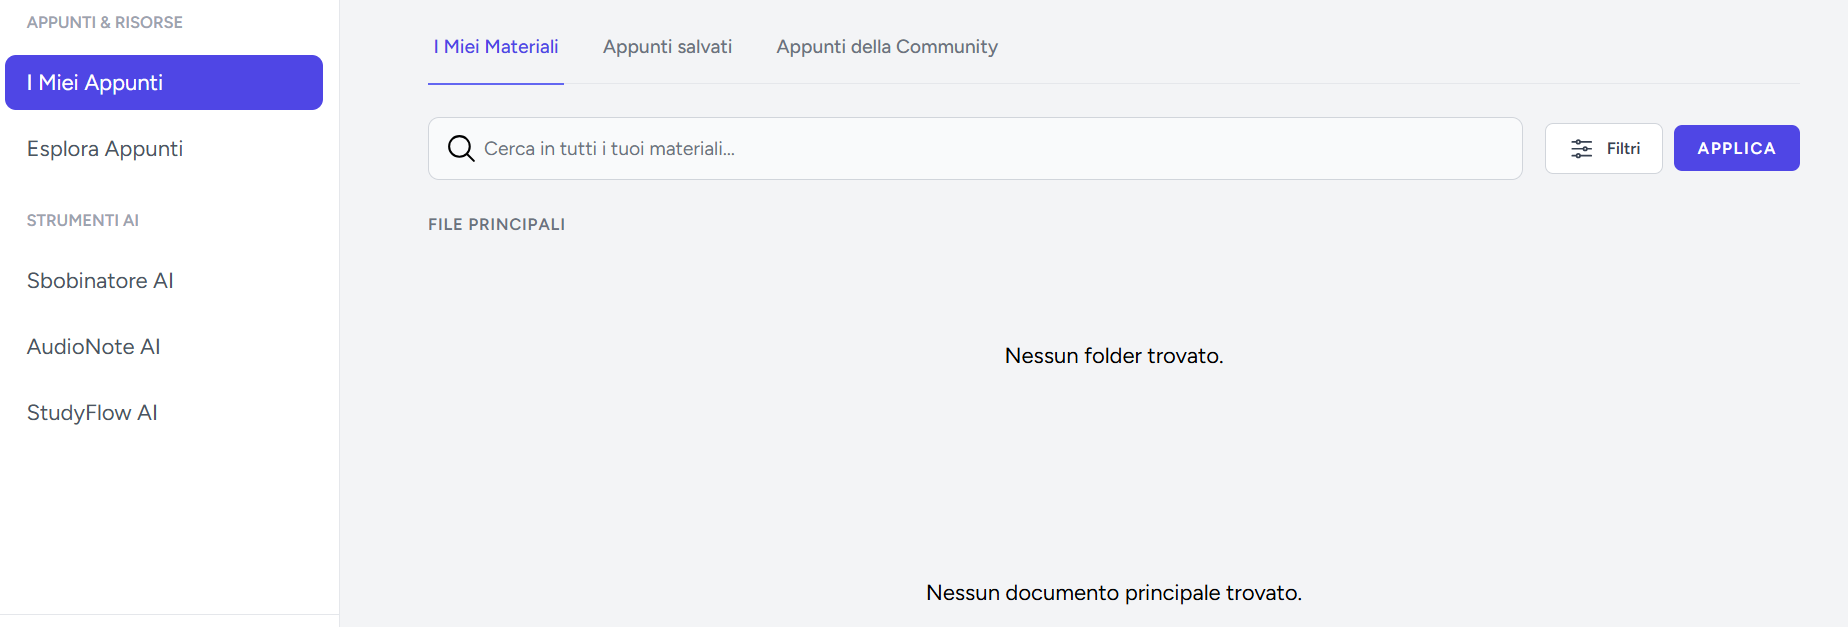
\includegraphics[width=6.5cm]{Screenshots/foglio2/problema029.png}\hspace*{\fill}
    \vspace{10pt}
    \\
    \hline
    \textbf{Nome del valutatore} & Kharef \\
    \hline
  \end{tabular}
\end{table}

\FloatBarrier

% Problema \getNumeroProblema (Basato su Kharef P3)
\begin{table}[htbp]
  \centering
  \renewcommand{\arraystretch}{1.5}
  \begin{tabular}{|>{\raggedright\arraybackslash}p{7.5cm}|>{\raggedright\arraybackslash}p{7.5cm}|}
    \hline
    \rowcolor{green!30}
    \multicolumn{2}{|c|}{\textbf{Problema \getNumeroProblema}} \\
    \hline
    \textbf{Descrizione} & La funzionalità di ricerca nella pagina "Esplora Appunti" è limitata al solo titolo del documento. \\
    \hline
    \textbf{Pagina del sito} & Esplora Appunti \\
    \hline
    \textbf{Principi violati} & 6 (Flessibilità ed efficienza d'uso) \\
    \hline
    \textbf{Grado di severità} & 3 (Problema rilevante)  \\
    \hline
    \textbf{Nome del valutatore} & Kharef  \\
    \hline
  \end{tabular}
\end{table}

% Problema \getNumeroProblema (Basato su Kharef P4)
\begin{table}[htbp]
  \centering
  \renewcommand{\arraystretch}{1.5}
  \begin{tabular}{|>{\raggedright\arraybackslash}p{7.5cm}|>{\raggedright\arraybackslash}p{7.5cm}|}
    \hline
    \rowcolor{green!30}
    \multicolumn{2}{|c|}{\textbf{Problema \getNumeroProblema}} \\
    \hline
    \textbf{Descrizione} & L'azione di caricare un nuovo documento è accessibile solo dalla pagina "I Miei Appunti". Non è presente un pulsante di accesso rapido ("Carica" o "+") nella barra di navigazione principale o nella dashboard. \\
    \hline
    \textbf{Pagina del sito} & Dashboard \\
    \hline
    \textbf{Principi violati} & 4 (Assicurare consistenza); 6 (Assicurare flessibilità ed efficienza d’uso) \\
    \hline
    \textbf{Grado di severità} & 2 (Problema secondario)  \\
    \hline
    \textbf{Screen} &
    \vspace{10pt}
    \hspace*{\fill}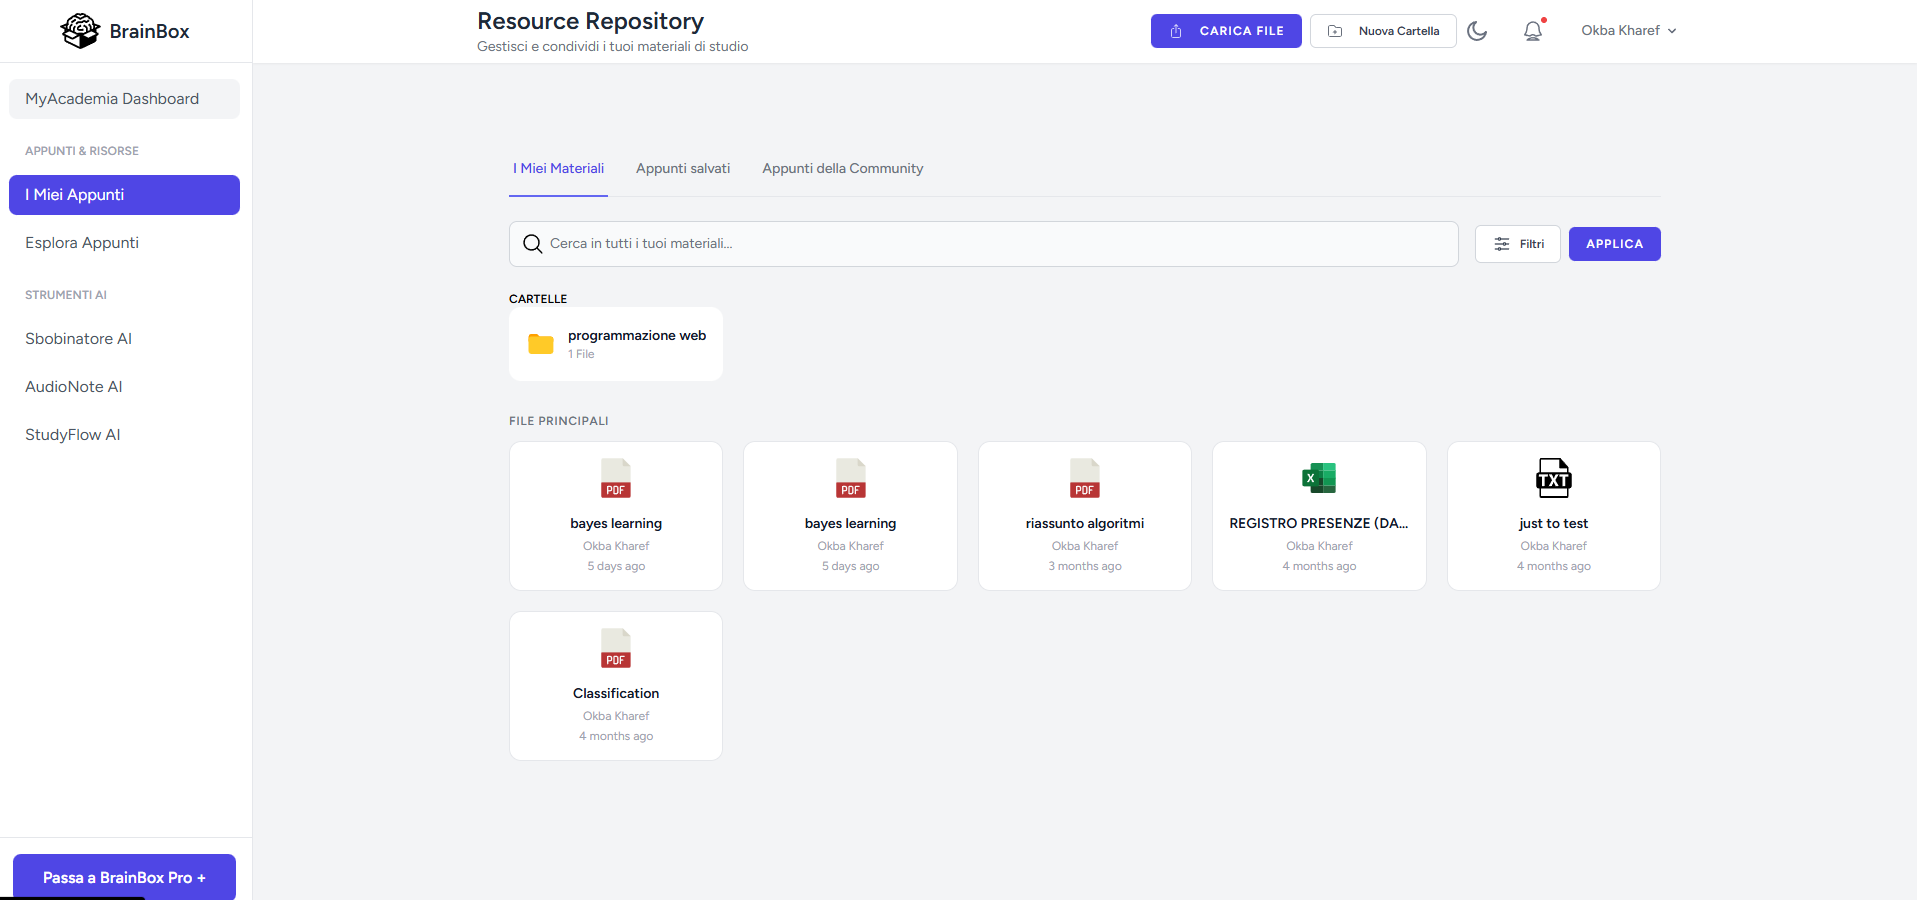
\includegraphics[width=6.5cm]{Screenshots/foglio3/problema62.png}\hspace*{\fill}
    \vspace{10pt}
    \\
    \hline
    \textbf{Nome del valutatore} & Kharef \\
    \hline
  \end{tabular}
\end{table}

% Problema \getNumeroProblema (Basato su Kharef P6)
\begin{table}[htbp]
  \centering
  \renewcommand{\arraystretch}{1.5}
  \begin{tabular}{|>{\raggedright\arraybackslash}p{7.5cm}|>{\raggedright\arraybackslash}p{7.5cm}|}
    \hline
    \rowcolor{green!30}
    \multicolumn{2}{|c|}{\textbf{Problema \getNumeroProblema}} \\
    \hline
    \textbf{Descrizione} & Il processo di registrazione in due fasi non fornisce indicatori di progresso (es. "Passo 1 di 2"). L'utente non sa che ci sarà un secondo passaggio, il che rende l'apparizione del secondo form inaspettata. \\
    \hline
    \textbf{Pagina del sito} & Registrazione \\
    \hline
    \textbf{Principi violati} & 1 (Visibilità dello stato del sistema); 3 (Controllo dell’utente e libertà) \\
    \hline
    \textbf{Grado di severità} & 3 (Problema rilevante) \\
    \hline
    \textbf{Screen} &
    \vspace{10pt}
    \hspace*{\fill}
    \begin{minipage}{0.48\linewidth}
      \centering
      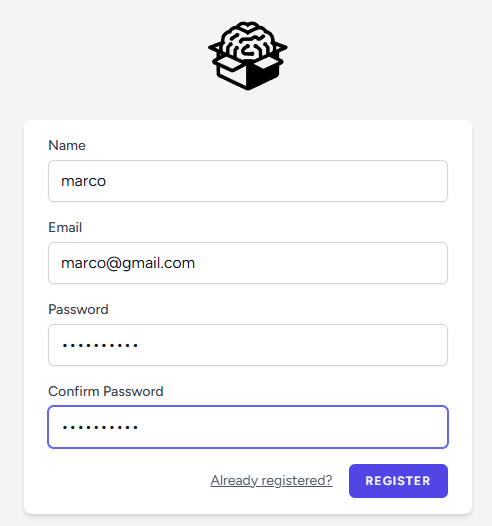
\includegraphics[width=3.5cm]{Screenshots/foglio3/problema64a.png}
    \end{minipage}
    \hfill
    \begin{minipage}{0.48\linewidth}
      \centering
      
\includegraphics[width=3.5cm]{Screenshots/foglio3/problema64b.png}
    \end{minipage}
    \hspace*{\fill}
    \vspace{10pt}
    \\
    \hline
    \textbf{Nome del valutatore} & Kharef \\
    \hline
  \end{tabular}
\end{table}

% Problema \getNumeroProblema (Basato su Kharef P7)
\begin{table}[htbp]
  \centering
  \renewcommand{\arraystretch}{1.5}
  \begin{tabular}{|>{\raggedright\arraybackslash}p{7.5cm}|>{\raggedright\arraybackslash}p{7.5cm}|}
    \hline
    \rowcolor{green!30}
    \multicolumn{2}{|c|}{\textbf{Problema \getNumeroProblema}} \\
    \hline
    \textbf{Descrizione} & Manca consistenza nella terminologia delle azioni. Nella pagina "I Miei Appunti", l'azione primaria si chiama "Scarica", ma all'interno della pagina dettaglio si chiama "download". \\
    \hline
    \textbf{Pagina del sito} & I Miei Appunti \\
    \hline
    \textbf{Principi violati} & 2 (Adeguare il sistema al mondo reale); 4 (Assicurare consistenza)  \\
    \hline
    \textbf{Grado di severità} & 2 (Problema secondario)  \\
    \hline
    \textbf{Screen} &
    \vspace{10pt}
    \hspace*{\fill}
    \begin{minipage}{0.48\linewidth}
      \centering
      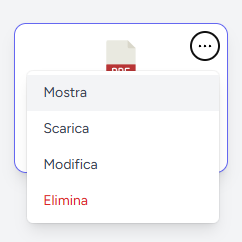
\includegraphics[width=3.5cm]{Screenshots/foglio3/problema65a.png}
    \end{minipage}
    \hfill
    \begin{minipage}{0.48\linewidth}
      \centering
      
\includegraphics[width=3.5cm]{Screenshots/foglio3/problema65b.png}
    \end{minipage}
    \hspace*{\fill}
    \vspace{10pt}
    \\
    \hline
    \textbf{Nome del valutatore} & Kharef \\
    \hline
  \end{tabular}
\end{table}

% Problema \getNumeroProblema (Basato su Kharef P10)
\begin{table}[htbp]
  \centering
  \renewcommand{\arraystretch}{1.5}
  \begin{tabular}{|>{\raggedright\arraybackslash}p{7.5cm}|>{\raggedright\arraybackslash}p{7.5cm}|}
    \hline
    \rowcolor{green!30}
    \multicolumn{2}{|c|}{\textbf{Problema \getNumeroProblema}} \\
    \hline
    \textbf{Descrizione} & Dopo aver caricato con successo un nuovo appunto, l'utente viene reindirizzato alla lista "I Miei Appunti", ma non c'è nessuna indicazione visiva (es. un'evidenziazione temporanea) che indichi quale sia il nuovo elemento appena aggiunto. \\
    \hline
    \textbf{Pagina del sito} & I Miei Appunti \\
    \hline
    \textbf{Principi violati} & 1 (Far vedere lo stato del sistema)\\
    \hline
    \textbf{Grado di severità} & 1 (Problema accessorio) \\
    \hline
    \textbf{Screen} &
    \vspace{10pt}
    \hspace*{\fill}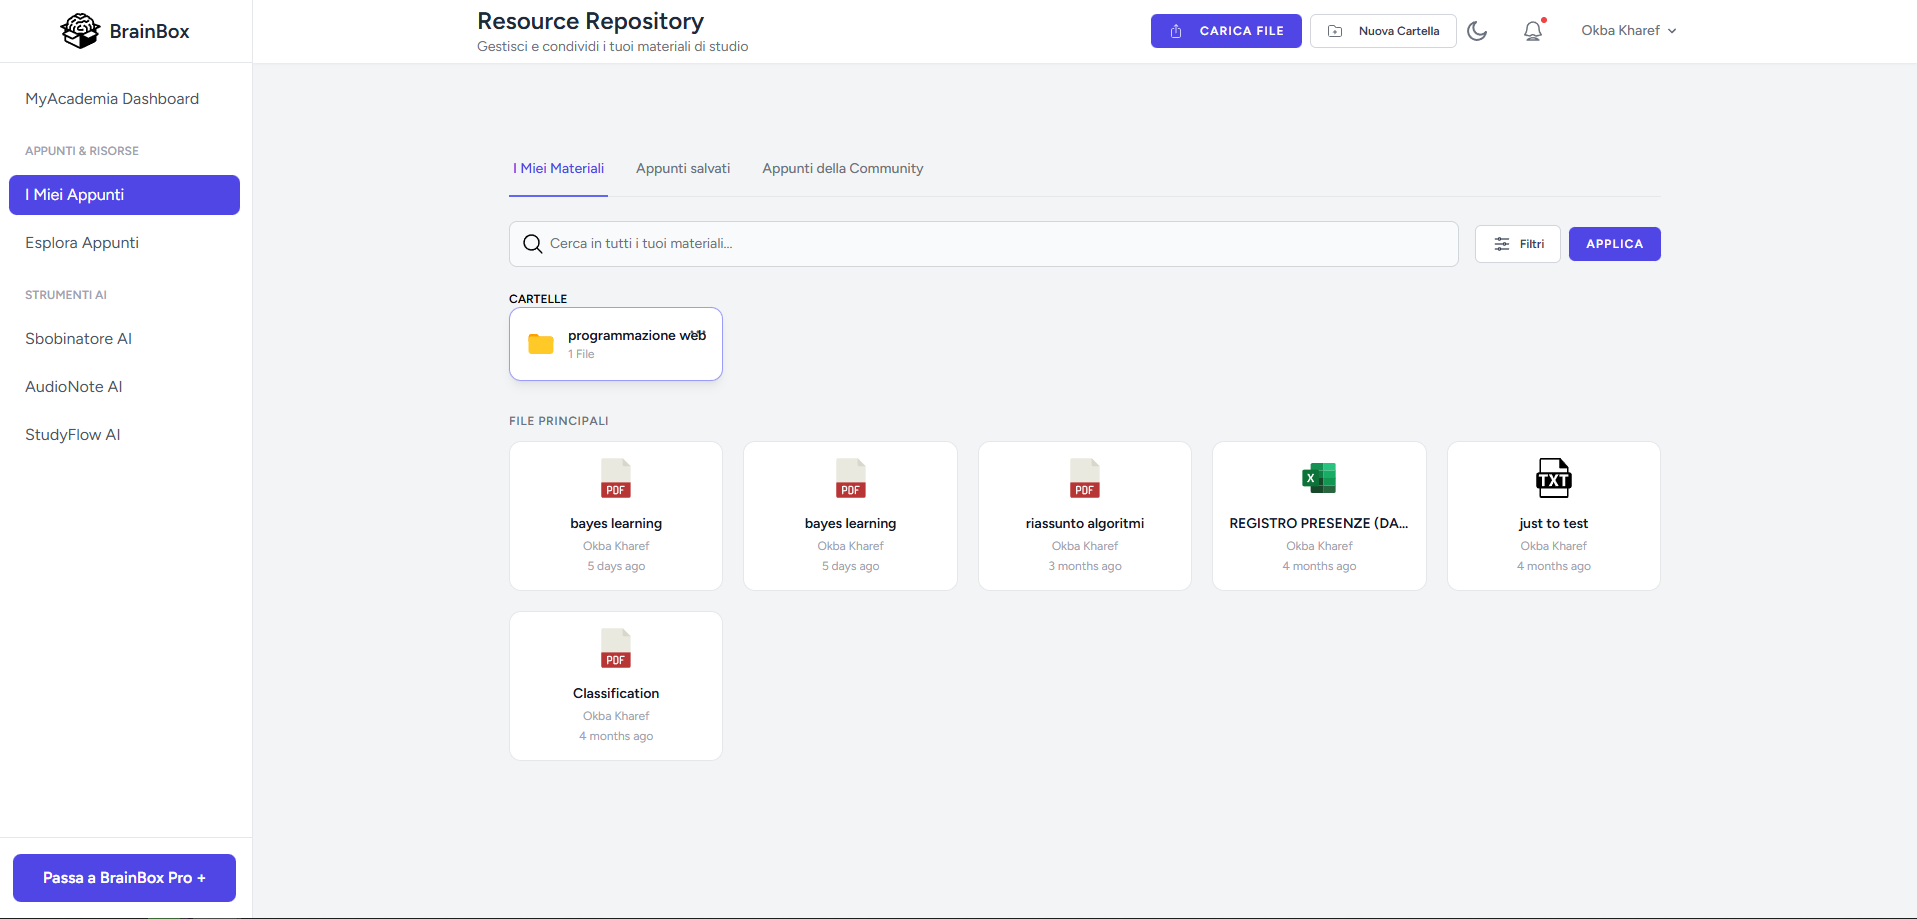
\includegraphics[width=6.5cm]{Screenshots/foglio3/problema68.png}\hspace*{\fill}
    \vspace{10pt}
    \\
    \hline
    \textbf{Nome del valutatore} & Kharef \\
    \hline
  \end{tabular}
\end{table}

% Problema \getNumeroProblema (Basato su Kharef P11)
\begin{table}[htbp]
  \centering
  \renewcommand{\arraystretch}{1.5}
  \begin{tabular}{|>{\raggedright\arraybackslash}p{7.5cm}|>{\raggedright\arraybackslash}p{7.5cm}|}
    \hline
    \rowcolor{green!30}
    \multicolumn{2}{|c|}{\textbf{Problema \getNumeroProblema}} \\
    \hline
    \textbf{Descrizione} & L'utente non ha alcun controllo sull'ordinamento delle liste di documenti (né in "I Miei Appunti" né in "Esplora Appunti"). I risultati sono presentati in un ordine predefinito senza opzioni di ordinamento (es. per popolarità, titolo, autore). \\
    \hline
    \textbf{Pagina del sito} & I Miei Appunti / Esplora Appunti \\
    \hline
    \textbf{Principi violati} & 3 (Controllo dell’utente e libertà); 6 (Assicurare flessibilità ed efficienza d’uso) \\
    \hline
    \textbf{Grado di severità} & 2 (Problema secondario) \\
    \hline
    \textbf{Screen} &
    \vspace{10pt}
    \hspace*{\fill}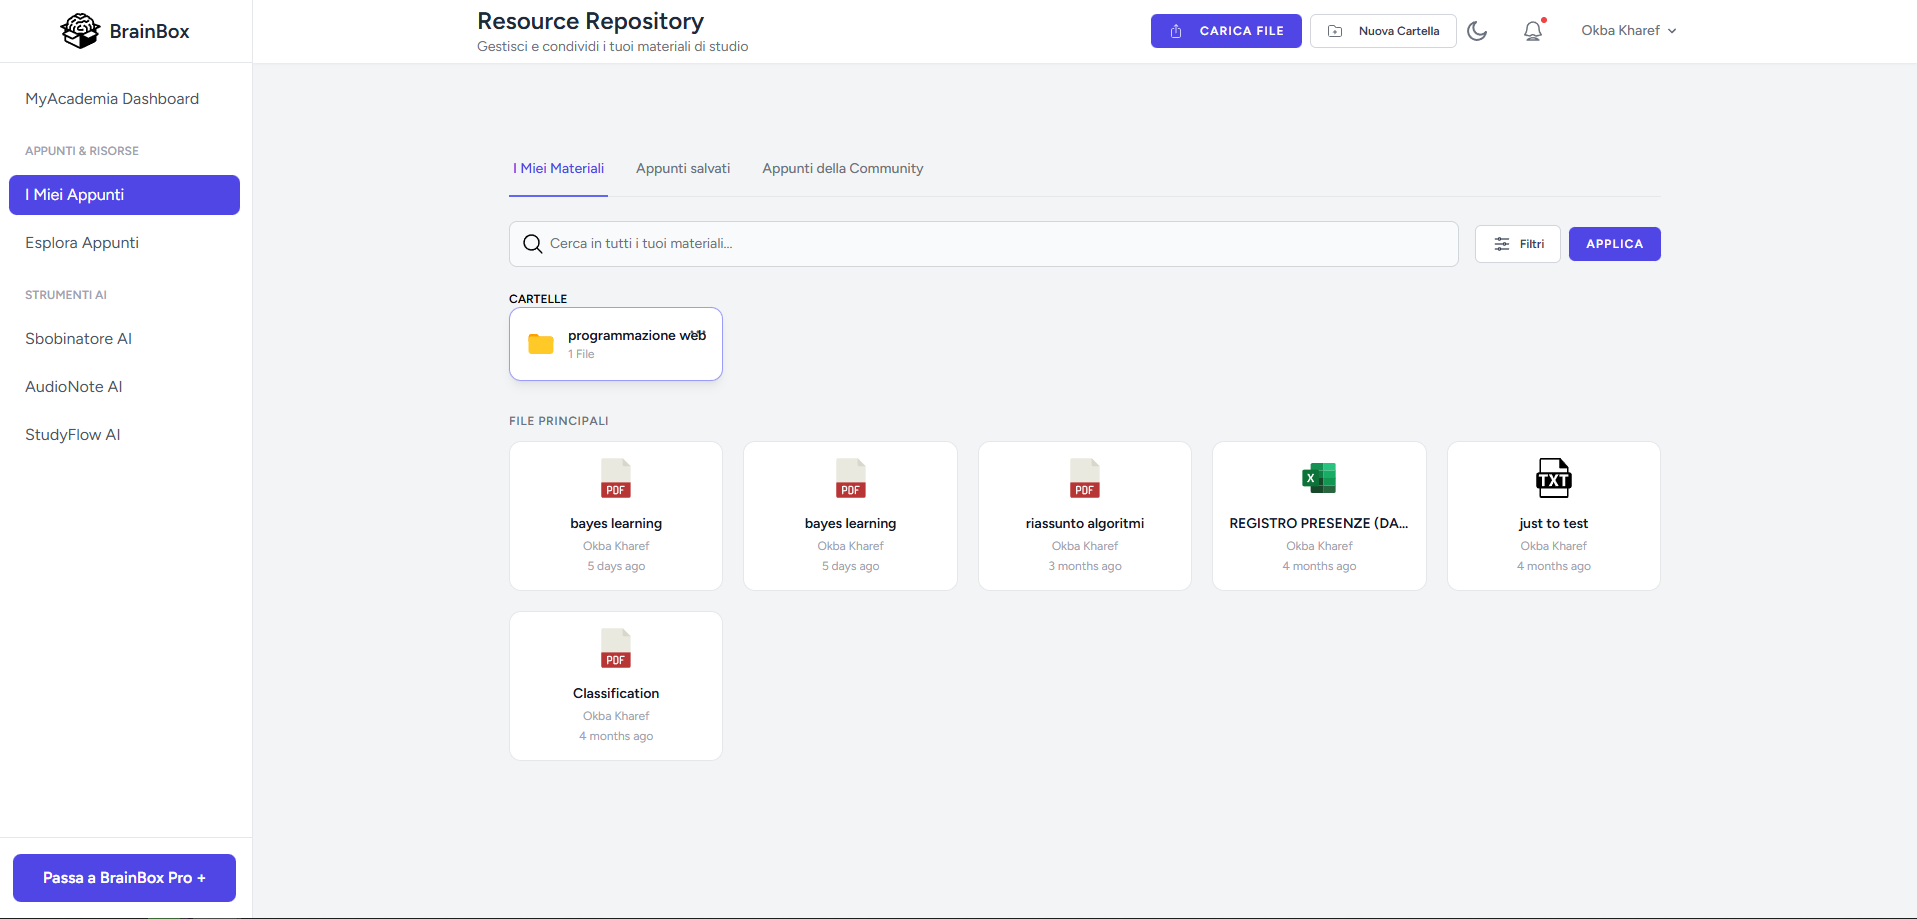
\includegraphics[width=6.5cm]{Screenshots/foglio3/problema68.png}\hspace*{\fill}
    \vspace{10pt}
    \\
    \hline
    \textbf{Nome del valutatore} & Kharef \\
    \hline
  \end{tabular}
\end{table}

% Problema \getNumeroProblema (Basato su Kharef P13)
\begin{table}[htbp]
  \centering
  \renewcommand{\arraystretch}{1.5}
  \begin{tabular}{|>{\raggedright\arraybackslash}p{7.5cm}|>{\raggedright\arraybackslash}p{7.5cm}|}
    \hline
    \rowcolor{green!30}
    \multicolumn{2}{|c|}{\textbf{Problema \getNumeroProblema}} \\
    \hline
    \textbf{Descrizione} & I messaggi di errore di validazione nei form, pur essendo presenti (es. Pagina "Sbobinatore AI"), sono generici e non sempre offrono una guida utile (es. "Il file non è valido" invece di "Il file supera la dimensione massima consentita"). \\
    \hline
    \textbf{Pagina del sito} & Area Utente \\
    \hline
    \textbf{Principi violati} & 1 (Far vedere lo stato del sistema); 9 (Permettere all’utente di correggere gli errori e non solo di rilevarli) \\
    \hline
    \textbf{Grado di severità} & 2 (Problema secondario) \\
    \hline
    \textbf{Nome del valutatore} & Kharef \\
    \hline
  \end{tabular}
\end{table}

% Problema \getNumeroProblema (Basato su Kharef P14)
\begin{table}[htbp]
  \centering
  \renewcommand{\arraystretch}{1.5}
  \begin{tabular}{|>{\raggedright\arraybackslash}p{7.5cm}|>{\raggedright\arraybackslash}p{7.5cm}|}
    \hline
    \rowcolor{green!30}
    \multicolumn{2}{|c|}{\textbf{Problema \getNumeroProblema}} \\
    \hline
    \textbf{Descrizione} & I messaggi di errore di validazione nei form non sono presenti se si tenta di caricare un file multimediale non supportato (ad esempio, nella Pagina "Sbobinatore AI"). \\
    \hline
    \textbf{Pagina del sito} & Area Utente \\
    \hline
    \textbf{Principi violati} & 1 (Far vedere lo stato del sistema); 9 (Permettere all’utente di correggere gli errori e non solo di rilevarli) \\
    \hline
    \textbf{Grado di severità} & 3 (Problema rilevante) \\
    \hline
    \textbf{Screen} &
    \vspace{10pt}
    \hspace*{\fill}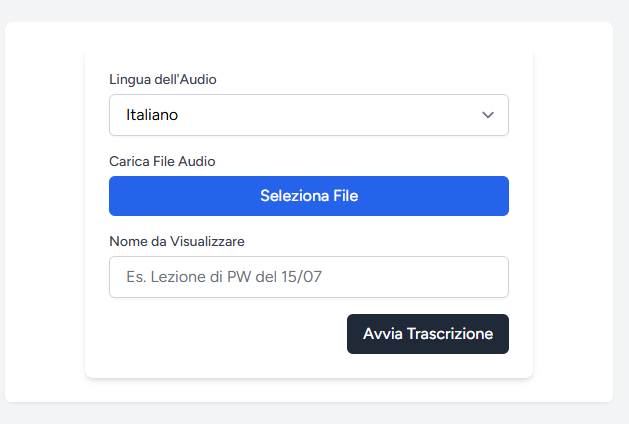
\includegraphics[width=6.5cm]{Screenshots/foglio3/problema72.png}\hspace*{\fill}
    \vspace{10pt}
    \\
    \hline
    \textbf{Nome del valutatore} & Kharef \\
    \hline
  \end{tabular}
\end{table}

% Problema \getNumeroProblema (Basato su Kharef P15)
\begin{table}[htbp]
  \centering
  \renewcommand{\arraystretch}{1.5}
  \begin{tabular}{|>{\raggedright\arraybackslash}p{7.5cm}|>{\raggedright\arraybackslash}p{7.5cm}|}
    \hline
    \rowcolor{green!30}
    \multicolumn{2}{|c|}{\textbf{Problema \getNumeroProblema}} \\
    \hline
    \textbf{Descrizione} & Nella pagina di dettaglio di un documento, non c'è una chiara separazione gerarchica tra i metadati del documento e la sezione dei commenti. Sono presentati come blocchi sequenziali di uguale importanza visiva. \\
    \hline
    \textbf{Pagina del sito} & I Miei Appunti - Visualizzazione Documento \\
    \hline
    \textbf{Principi violati} & 7 (Visualizzare tutte e sole le informazioni necessarie) \\
    \hline
    \textbf{Grado di severità} & 1 (Problema accessorio) \\
    \hline
    \textbf{Screen} &
    \vspace{10pt}
    \hspace*{\fill}
\includegraphics[height=6cm, keepaspectratio]{Screenshots/foglio3/problema73.png}\hspace*{\fill}
    \vspace{10pt}
    \\
    \hline
    \textbf{Nome del valutatore} & Kharef \\
    \hline
  \end{tabular}
\end{table}

% Problema \getNumeroProblema (Basato su Kharef P16)
\begin{table}[htbp]
  \centering
  \renewcommand{\arraystretch}{1.5}
  \begin{tabular}{|>{\raggedright\arraybackslash}p{7.5cm}|>{\raggedright\arraybackslash}p{7.5cm}|}
    \hline
    \rowcolor{green!30}
    \multicolumn{2}{|c|}{\textbf{Problema \getNumeroProblema}} \\
    \hline
    \textbf{Descrizione} & Non esiste un feedback visivo che distingua i link interni già visitati da quelli non ancora visitati, costringendo l'utente a ricordare quali contenuti ha già consultato. \\
    \hline
    \textbf{Pagina del sito} & I Miei Appunti / Esplora Appunti \\
    \hline
    \textbf{Principi violati} & 1 (Far vedere lo stato del sistema); 5 (Riconoscimento anziché ricordo) \\
    \hline
    \textbf{Grado di severità} & 1 (Problema accessorio) \\
    \hline
    \textbf{Screen} &
    \vspace{10pt}
    \hspace*{\fill}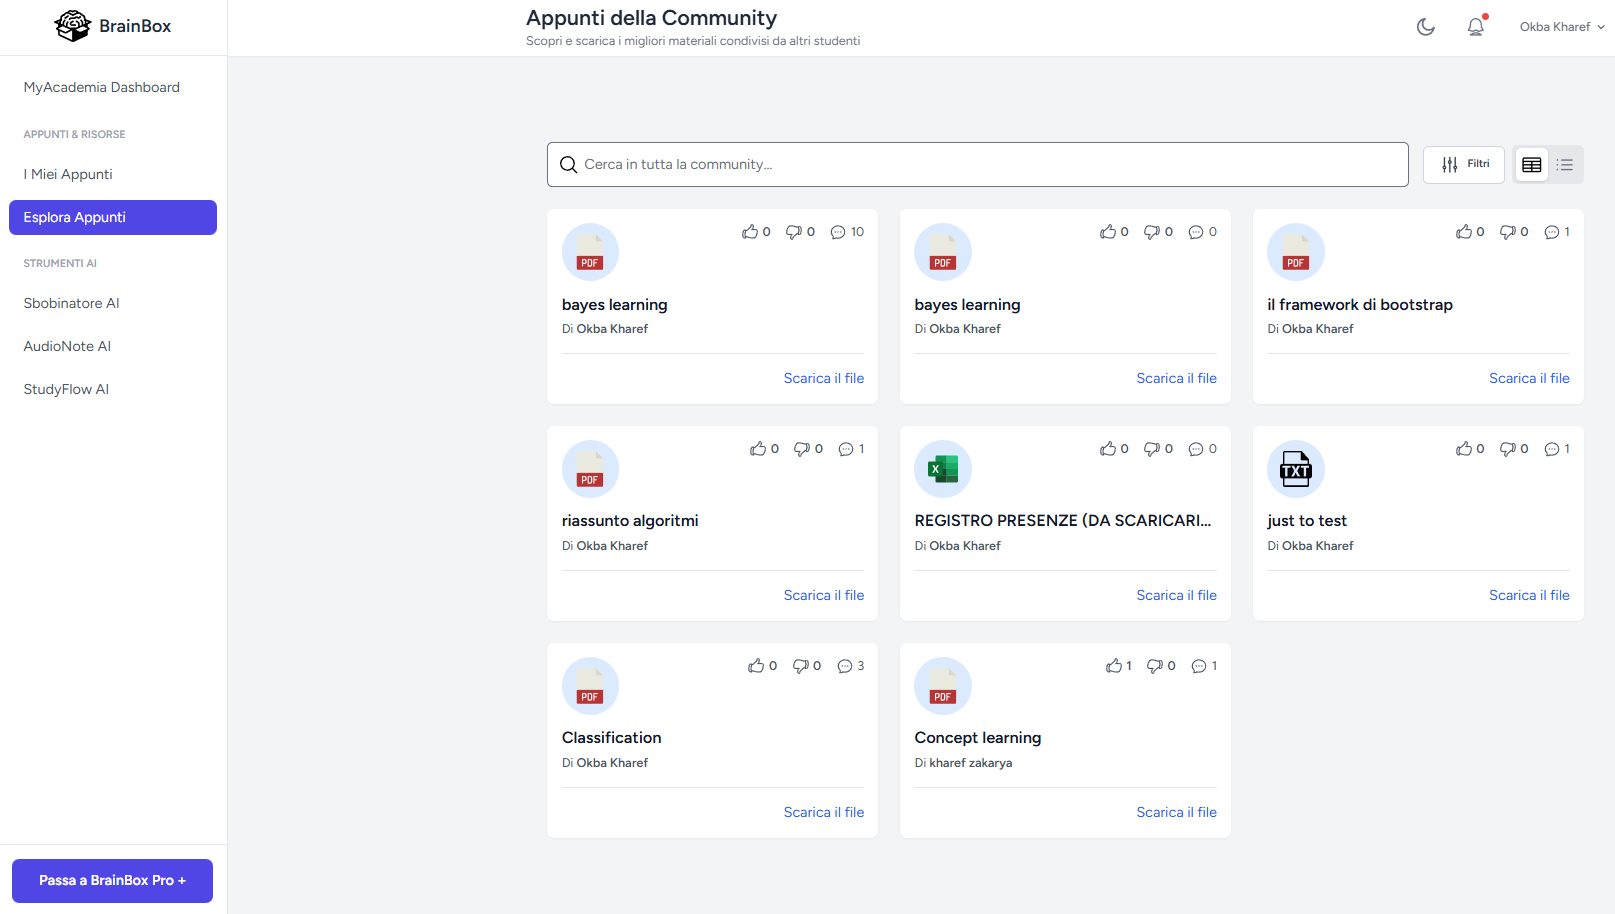
\includegraphics[width=6.5cm]{Screenshots/foglio3/problema74.png}\hspace*{\fill}
    \vspace{10pt}
    \\
    \hline
    \textbf{Nome del valutatore} & Kharef \\
    \hline
  \end{tabular}
\end{table}

% Problema \getNumeroProblema (Basato su Kharef P17)
\begin{table}[htbp]
  \centering
  \renewcommand{\arraystretch}{1.5}
  \begin{tabular}{|>{\raggedright\arraybackslash}p{7.5cm}|>{\raggedright\arraybackslash}p{7.5cm}|}
    \hline
    \rowcolor{green!30}
    \multicolumn{2}{|c|}{\textbf{Problema \getNumeroProblema}} \\
    \hline
    \textbf{Descrizione} & Non c'è modo per un utente di segnalare un commento o un documento inappropriato (es. offensivo, spam, violazione di copyright). \\
    \hline
    \textbf{Pagina del sito} & I Miei Appunti - Visualizzazione Documento \\
    \hline
    \textbf{Principi violati} & 3 (Controllo dell’utente e libertà) \\
    \hline
    \textbf{Grado di severità} & 2 (Problema rilevante) \\
    \hline
    \textbf{Nome del valutatore} & Kharef \\
    \hline
  \end{tabular}
\end{table}

% Problema \getNumeroProblema (Basato su Kharef P18)
\begin{table}[htbp]
  \centering
  \renewcommand{\arraystretch}{1.5}
  \begin{tabular}{|>{\raggedright\arraybackslash}p{7.5cm}|>{\raggedright\arraybackslash}p{7.5cm}|}
    \hline
    \rowcolor{green!30}
    \multicolumn{2}{|c|}{\textbf{Problema \getNumeroProblema}} \\
    \hline
    \textbf{Descrizione} & Il sistema non offre alcuna forma di salvataggio automatico o bozza. Il lavoro (descrizioni lunghe o commenti complessi) può essere perso in caso di caduta della connessione o chiusura accidentale della pagina. \\
    \hline
    \textbf{Pagina del sito} & I Miei Appunti \\
    \hline
    \textbf{Principi violati} & 8 (Prevenire gli errori) \\
    \hline
    \textbf{Grado di severità} & 3 (Problema rilevante)  \\
    \hline
    \textbf{Nome del valutatore} & Kharef \\
    \hline
  \end{tabular}
\end{table}

% Problema \getNumeroProblema (Basato su Kharef P20)
\begin{table}[htbp]
  \centering
  \renewcommand{\arraystretch}{1.5}
  \begin{tabular}{|>{\raggedright\arraybackslash}p{7.5cm}|>{\raggedright\arraybackslash}p{7.5cm}|}
    \hline
    \rowcolor{green!30}
    \multicolumn{2}{|c|}{\textbf{Problema \getNumeroProblema}} \\
    \hline
    \textbf{Descrizione} & I titoli dei file scaricati non sono formattati, il file scaricato ha un nome casuale (es. aGDvnS4viFvc9VSHFJDdA5dE6HvmkjshP hkiVCBV.pdf) invece di usare un nome descrittivo basato sul titolo del documento (es. Riassunto\_Analisi\_1-BrainBox.pdf). \\
    \hline
    \textbf{Pagina del sito} & Area Utente \\
    \hline
    \textbf{Principi violati} & 2 (Adeguare il sistema al mondo reale); 7 (Visualizzare tutte e sole le informazioni necessarie) \\
    \hline
    \textbf{Grado di severità} & 2 (Problema secondario) \\
    \hline
    \textbf{Screen} &
    \vspace{10pt}
    \hspace*{\fill}
\includegraphics[width=6.5cm]{Screenshots/foglio3/problema78.png}\hspace*{\fill}
    \vspace{10pt}
    \\
    \hline
    \textbf{Nome del valutatore} & Kharef \\
    \hline
  \end{tabular}
\end{table}

% Problema \getNumeroProblema (Basato su Kharef P22)
\begin{table}[htbp]
  \centering
  \renewcommand{\arraystretch}{1.5}
  \begin{tabular}{|>{\raggedright\arraybackslash}p{7.5cm}|>{\raggedright\arraybackslash}p{7.5cm}|}
    \hline
    \rowcolor{green!30}
    \multicolumn{2}{|c|}{\textbf{Problema \getNumeroProblema}} \\
    \hline
    \textbf{Descrizione} & Su schermi di dispositivi mobili, la modifica dei commenti causa problemi di visualizzazione. Quando si modifica un commento, la pagina si riorganizza in modo confuso, gli elementi si spostano e la barra laterale non si adatta correttamente. \\
    \hline
    \textbf{Pagina del sito} & I Miei Appunti - Visualizzazione Documento \\
    \hline
    \textbf{Principi violati} & 3 (Controllo dell’utente e libertà); 7 (Visualizzare tutte e sole le informazioni necessarie) \\
    \hline
    \textbf{Grado di severità} & 2 (Problema secondario) \\
    \hline
    \textbf{Screen} &
    \vspace{10pt}
    \hspace*{\fill}
\includegraphics[height=6cm, keepaspectratio]{Screenshots/foglio3/problema80.png}\hspace*{\fill}
    \vspace{10pt}
    \\
    \hline
    \textbf{Nome del valutatore} & Kharef \\
    \hline
  \end{tabular}
\end{table}

% Problema \getNumeroProblema (Basato su Kharef P23)
\begin{table}[htbp]
  \centering
  \renewcommand{\arraystretch}{1.5}
  \begin{tabular}{|>{\raggedright\arraybackslash}p{7.5cm}|>{\raggedright\arraybackslash}p{7.5cm}|}
    \hline
    \rowcolor{green!30}
    \multicolumn{2}{|c|}{\textbf{Problema \getNumeroProblema}} \\
    \hline
    \textbf{Descrizione} & Le funzionalità AI operano in completo isolamento. Non esiste un pulsante o un'azione per "Salvare come nuovo appunto" la trascrizione, o per "Allegare questa nota audio" a un task. \\
    \hline
    \textbf{Pagina del sito} & Sbobinatore AI / AudioNote AI \\
    \hline
    \textbf{Principi violati} & 4 (Assicurare consistenza); 6 (Assicurare flessibilità ed efficienza d’uso) \\
    \hline
    \textbf{Grado di severità} & 3 (Problema rilevante) \\
    \hline
    \textbf{Nome del valutatore} & Kharef \\
    \hline
  \end{tabular}
\end{table}

% Problema \getNumeroProblema (Basato su Kharef P25)
\begin{table}[htbp]
  \centering
  \renewcommand{\arraystretch}{1.5}
  \begin{tabular}{|>{\raggedright\arraybackslash}p{7.5cm}|>{\raggedright\arraybackslash}p{7.5cm}|}
    \hline
    \rowcolor{green!30}
    \multicolumn{2}{|c|}{\textbf{Problema \getNumeroProblema}} \\
    \hline
    \textbf{Descrizione} & L'interfaccia si affida quasi esclusivamente a etichette testuali, mancando di un supporto iconografico. \\
    \hline
    \textbf{Pagina del sito} & AudioNote AI \\
    \hline
    \textbf{Principi violati} & 1 (Far vedere lo stato del sistema); 2 (Adeguare il sistema al mondo reale) \\
    \hline
    \textbf{Grado di severità} & 1 (Problema accessorio) \\
    \hline
    \textbf{Screen} &
    \vspace{10pt}
    \hspace*{\fill}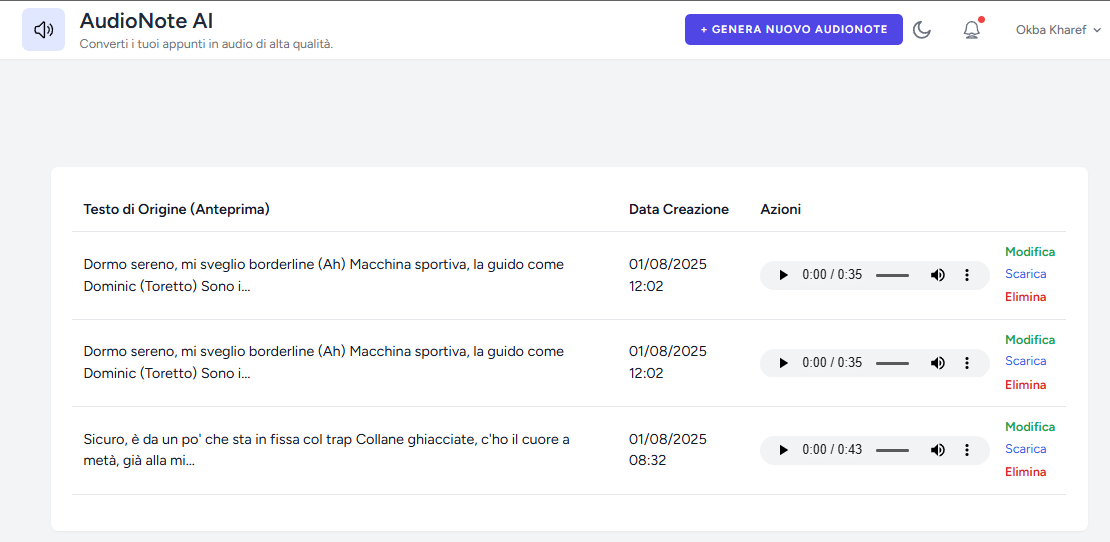
\includegraphics[width=6.5cm]{Screenshots/foglio3/problema83.png}\hspace*{\fill}
    \vspace{10pt}
    \\
    \hline
    \textbf{Nome del valutatore} & Kharef \\
    \hline
  \end{tabular}
\end{table}

% Problema \getNumeroProblema (Basato su Kharef P27)
\begin{table}[htbp]
  \centering
  \renewcommand{\arraystretch}{1.5}
  \begin{tabular}{|>{\raggedright\arraybackslash}p{7.5cm}|>{\raggedright\arraybackslash}p{7.5cm}|}
    \hline
    \rowcolor{green!30}
    \multicolumn{2}{|c|}{\textbf{Problema \getNumeroProblema}} \\
    \hline
    \textbf{Descrizione} & I contenuti generati dagli strumenti AI (trascrizioni e AudioNote) sono presentati come output "finali" e non modificabili. \\
    \hline
    \textbf{Pagina del sito} & Sbobinatore AI / AudioNote AI \\
    \hline
    \textbf{Principi violati} & 3 (Controllo e libertà dell'utente); 9 (Permettere all’utente di correggere gli errori e non solo di rilevarli) \\
    \hline
    \textbf{Grado di severità} & 2 (Problema secondario) \\
    \hline
    \textbf{Screen} &
    \vspace{10pt}
    \hspace*{\fill}
\includegraphics[width=6.5cm]{Screenshots/foglio3/problema85.png}\hspace*{\fill}
    \vspace{10pt}
    \\
    \hline
    \textbf{Nome del valutatore} & Kharef \\
    \hline
  \end{tabular}
\end{table}

% Problema \getNumeroProblema (Basato su Kharef P29)
\begin{table}[htbp]
  \centering
  \renewcommand{\arraystretch}{1.5}
  \begin{tabular}{|>{\raggedright\arraybackslash}p{7.5cm}|>{\raggedright\arraybackslash}p{7.5cm}|}
    \hline
    \rowcolor{green!30}
    \multicolumn{2}{|c|}{\textbf{Problema \getNumeroProblema}} \\
    \hline
    \textbf{Descrizione} & Non è presente una chiara distinzione visiva tra le proprie risorse (appunti caricati dall'utente) e le risorse della community quando si naviga in "Esplora Appunti". \\
    \hline
    \textbf{Pagina del sito} & Esplora Appunti \\
    \hline
    \textbf{Principi violati} & 1 (Far vedere lo stato del sistema); 5 (Riconoscimento piuttosto che uso della memoria dell’utente); 7 (Visualizzare tutte e sole le informazioni necessarie) \\
    \hline
    \textbf{Grado di severità} & 1 (Problema accessorio) \\
    \hline
    \textbf{Screen} &
    \vspace{10pt}
    \hspace*{\fill}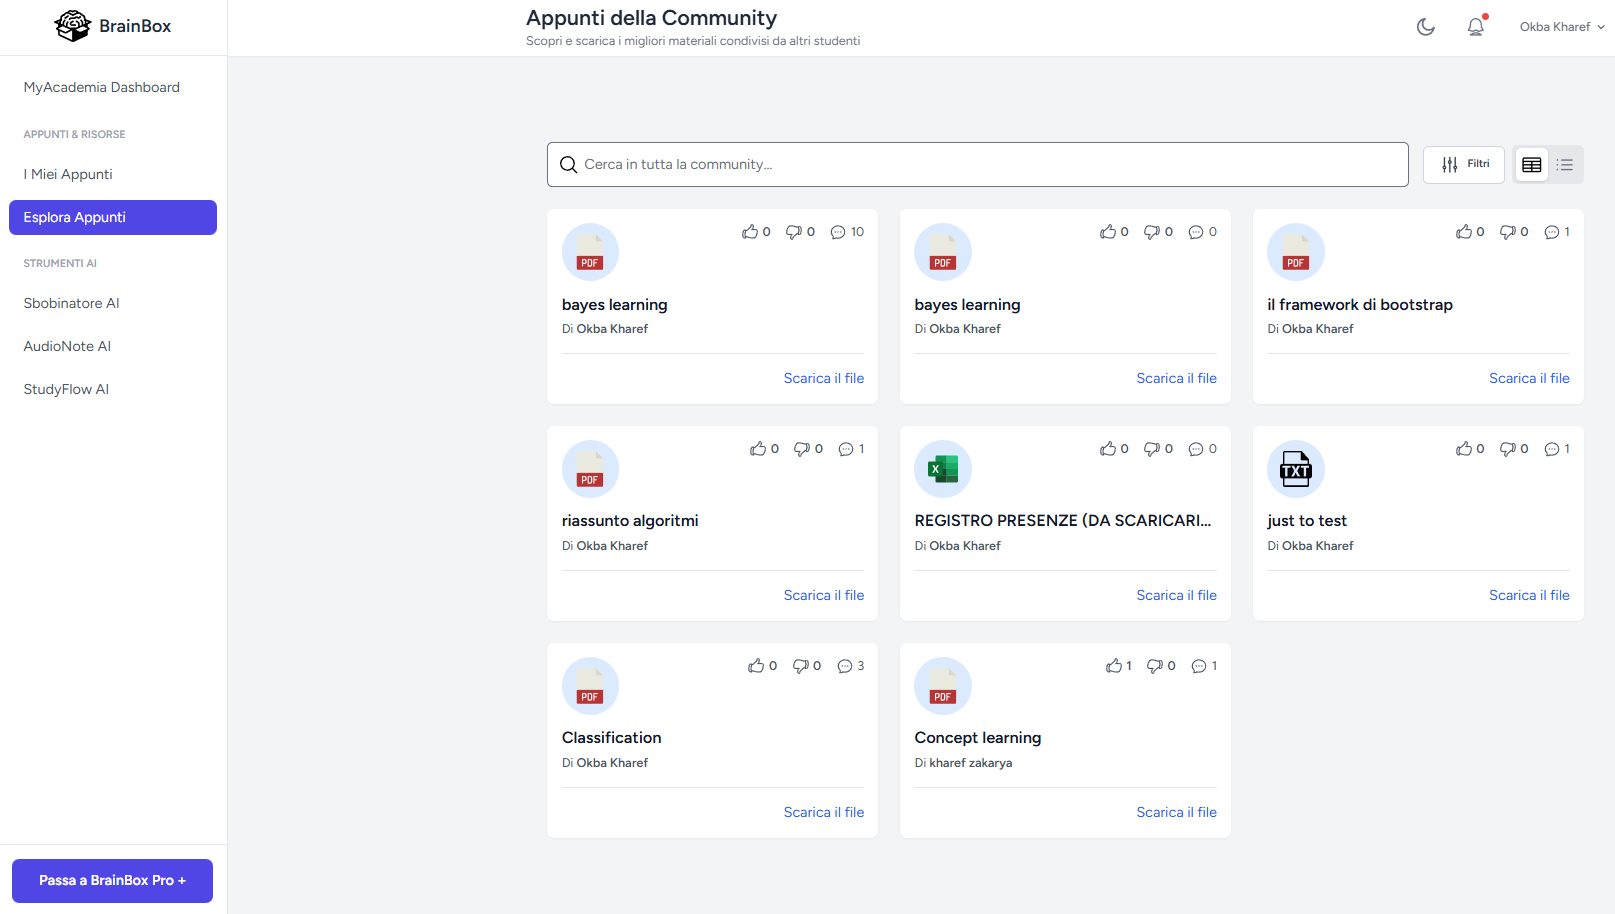
\includegraphics[width=6.5cm]{Screenshots/foglio3/problema74.png}\hspace*{\fill}
    \vspace{10pt}
    \\
    \hline
    \textbf{Nome del valutatore} & Kharef \\
    \hline
  \end{tabular}
\end{table}

% Problema \getNumeroProblema (Basato su Kharef P30)
\begin{table}[htbp]
  \centering
  \renewcommand{\arraystretch}{1.5}
  \begin{tabular}{|>{\raggedright\arraybackslash}p{7.5cm}|>{\raggedright\arraybackslash}p{7.5cm}|}
    \hline
    \rowcolor{green!30}
    \multicolumn{2}{|c|}{\textbf{Problema \getNumeroProblema}} \\
    \hline
    \textbf{Descrizione} & Le funzionalità basate su AI (Sbobinatore e Generatore AudioNote) non spiegano i loro limiti tecnologici (es. la qualità dipende dall'audio, la voce generata è sintetica), creando aspettative irrealistiche. \\
    \hline
    \textbf{Pagina del sito} & Sbobinatore AI / AudioNote AI  \\
    \hline
    \textbf{Principi violati} & 1 (Far vedere lo stato del sistema); 10 (Help e documentazione) \\
    \hline
    \textbf{Grado di severità} & 2 (Problema secondario)  \\
    \hline
    \textbf{Nome del valutatore} & Kharef \\
    \hline
  \end{tabular}
\end{table}

% Problema \getNumeroProblema (Basato su Kharef P32)
\begin{table}[htbp]
  \centering
  \renewcommand{\arraystretch}{1.5}
  \begin{tabular}{|>{\raggedright\arraybackslash}p{7.5cm}|>{\raggedright\arraybackslash}p{7.5cm}|}
    \hline
    \rowcolor{green!30}
    \multicolumn{2}{|c|}{\textbf{Problema \getNumeroProblema}} \\
    \hline
    \textbf{Descrizione} & I testi inseriti dagli utenti (descrizione degli appunti o commenti) non supportano alcuna formattazione di base (grassetto, corsivo, elenchi). Questo porta alla creazione di "muri di testo" poco leggibili. \\
    \hline
    \textbf{Pagina del sito} & I Miei Appunti \\
    \hline
    \textbf{Principi violati} & 6 (Assicurare flessibilità ed efficienza d’uso); 7 (Visualizzare tutte e sole le informazioni necessarie) \\
    \hline
    \textbf{Grado di severità} & 1 (Problema accessorio) \\
    \hline
    \textbf{Screen} &
    \vspace{10pt}
    \hspace*{\fill}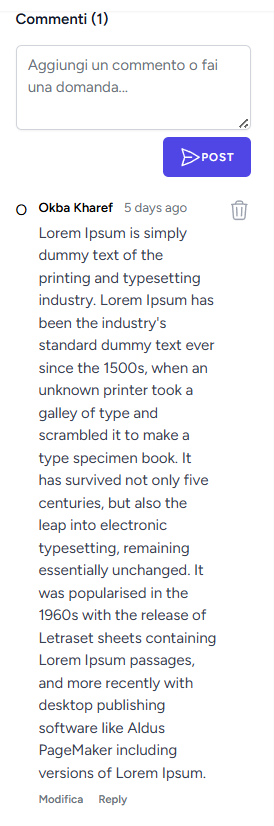
\includegraphics[height=6cm, keepaspectratio]{Screenshots/foglio3/problema90.png}\hspace*{\fill}
    \vspace{10pt}
    \\
    \hline
    \textbf{Nome del valutatore} & Kharef \\
    \hline
  \end{tabular}
\end{table}

\FloatBarrier

% Problema \getNumeroProblema (Basato su Kharef P35)
\begin{table}[htbp]
  \centering
  \renewcommand{\arraystretch}{1.5}
  \begin{tabular}{|>{\raggedright\arraybackslash}p{7.5cm}|>{\raggedright\arraybackslash}p{7.5cm}|}
    \hline
    \rowcolor{green!30}
    \multicolumn{2}{|c|}{\textbf{Problema \getNumeroProblema}} \\
    \hline
    \textbf{Descrizione} & Il sistema manca di strumenti organizzativi per la gestione di grandi quantità di documenti. Non esistono cartelle, sottocartelle personalizzate nella pagina "Esplora Appunti", rendendo l'uso ingestibile nel lungo periodo. \\
    \hline
    \textbf{Pagina del sito} & Esplora Appunti \\
    \hline
    \textbf{Principi violati} & 6 (Assicurare flessibilità ed efficienza d’uso); 7 (Visualizzare tutte e sole le informazioni necessarie) \\
    \hline
    \textbf{Grado di severità} & 3 (Problema rilevante) \\
    \hline
    \textbf{Nome del valutatore} & Kharef \\
    \hline
  \end{tabular}
\end{table}

% Problema \getNumeroProblema (Basato su Kharef P36)
\begin{table}[htbp]
  \centering
  \renewcommand{\arraystretch}{1.5}
  \begin{tabular}{|>{\raggedright\arraybackslash}p{7.5cm}|>{\raggedright\arraybackslash}p{7.5cm}|}
    \hline
    \rowcolor{green!30}
    \multicolumn{2}{|c|}{\textbf{Problema \getNumeroProblema}} \\
    \hline
    \textbf{Descrizione} & L'utente non può selezionare più documenti o trascrizioni o audio contemporaneamente per eseguire azioni comuni (es. caricare, eliminare, rendere pubblici/privati). \\
    \hline
    \textbf{Pagina del sito} & I Miei Appunti \\
    \hline
    \textbf{Principi violati} & 6 (Assicurare flessibilità ed efficienza d’uso) \\
    \hline
    \textbf{Grado di severità} & 2 (Problema secondario) \\
    \hline
    \textbf{Nome del valutatore} & Kharef \\
    \hline
  \end{tabular}
\end{table}

% Problema \getNumeroProblema (Basato su Kharef P38)
\begin{table}[htbp]
  \centering
  \renewcommand{\arraystretch}{1.5}
  \begin{tabular}{|>{\raggedright\arraybackslash}p{7.5cm}|>{\raggedright\arraybackslash}p{7.5cm}|}
    \hline
    \rowcolor{green!30}
    \multicolumn{2}{|c|}{\textbf{Problema \getNumeroProblema}} \\
    \hline
    \textbf{Descrizione} & Le trascrizioni generate dallo "Sbobinatore AI" mancano di struttura semantica. Sono presentate come un unico blocco di testo, senza timestamp che colleghino le frasi al punto corrispondente nel file audio. \\
    \hline
    \textbf{Pagina del sito} & Sbobinatore AI \\
    \hline
    \textbf{Principi violati} & 2 (Adeguare il sistema al mondo reale); 5 (Riconoscimento piuttosto che uso della memoria dell’utente) \\
    \hline
    \textbf{Grado di severità} & 3 (Problema rilevante) \\
    \hline
    \textbf{Screen} & 
    \vspace{10pt}
    \hspace*{\fill}
\includegraphics[width=6.5cm]{Screenshots/foglio3/problema85.png}\hspace*{\fill}
    \vspace{10pt}
    \\
    \hline
    \textbf{Nome del valutatore} & Kharef \\
    \hline
  \end{tabular}
\end{table}

% Problema \getNumeroProblema (Basato su Kharef P39)
\begin{table}[htbp]
  \centering
  \renewcommand{\arraystretch}{1.5}
  \begin{tabular}{|>{\raggedright\arraybackslash}p{7.5cm}|>{\raggedright\arraybackslash}p{7.5cm}|}
    \hline
    \rowcolor{green!30}
    \multicolumn{2}{|c|}{\textbf{Problema \getNumeroProblema}} \\
    \hline
    \textbf{Descrizione} & La ricerca è superficiale e non indicizza il contenuto dei file. Viene effettuata solo sui metadati (titolo, materia, descrizione), ignorando il testo contenuto all'interno dei file caricati. \\
    \hline
    \textbf{Pagina del sito} & Esplora Appunti \\
    \hline
    \textbf{Principi violati} & 2 (Adeguare il sistema al mondo reale); 7 (Visualizzare tutte e sole le informazioni necessarie) \\
    \hline
    \textbf{Grado di severità} & 2 (Problema secondario) \\
    \hline
    \textbf{Nome del valutatore} & Kharef \\
    \hline
  \end{tabular}
\end{table}

% Problema \getNumeroProblema (Basato su Kharef P40)
\begin{table}[htbp]
  \centering
  \renewcommand{\arraystretch}{1.5}
  \begin{tabular}{|>{\raggedright\arraybackslash}p{7.5cm}|>{\raggedright\arraybackslash}p{7.5cm}|}
    \hline
    \rowcolor{green!30}
    \multicolumn{2}{|c|}{\textbf{Problema \getNumeroProblema}} \\
    \hline
    \textbf{Descrizione} & La piattaforma non offre alcun tipo di funzionalità offline. L'accesso ai propri appunti, anche per la sola lettura, è completamente impedito senza una connessione internet stabile. \\
    \hline
    \textbf{Pagina del sito} & Globale \\
    \hline
    \textbf{Principi violati} & 3 (Controllo dell’utente e libertà) \\
    \hline
    \textbf{Grado di severità} & 2 (Problema secondario) \\
    \hline
    \textbf{Nome del valutatore} & Kharef \\
    \hline
  \end{tabular}
\end{table}

% Problema \getNumeroProblema (Basato su Kharef P41)
\begin{table}[htbp]
  \centering
  \renewcommand{\arraystretch}{1.5}
  \begin{tabular}{|>{\raggedright\arraybackslash}p{7.5cm}|>{\raggedright\arraybackslash}p{7.5cm}|}
    \hline
    \rowcolor{green!30}
    \multicolumn{2}{|c|}{\textbf{Problema \getNumeroProblema}} \\
    \hline
    \textbf{Descrizione} & Non c'è un modo per l'utente di vedere quali altri documenti ha caricato l'autore di un appunto, né ci sono suggerimenti automatici del tipo "Chi ha consultato questo appunto ha consultato anche...". \\
    \hline
    \textbf{Pagina del sito} & Esplora Appunti \\
    \hline
    \textbf{Principi violati} & 7 (Visualizzare tutte e sole le informazioni necessarie) \\
    \hline
    \textbf{Grado di severità} & 2 (Problema secondario) \\
    \hline
    \textbf{Nome del valutatore} & Kharef \\
    \hline
  \end{tabular}
\end{table}

% Problema \getNumeroProblema (Basato su Kharef P42)
\begin{table}[htbp]
  \centering
  \renewcommand{\arraystretch}{1.5}
  \begin{tabular}{|>{\raggedright\arraybackslash}p{7.5cm}|>{\raggedright\arraybackslash}p{7.5cm}|}
    \hline
    \rowcolor{green!30}
    \multicolumn{2}{|c|}{\textbf{Problema \getNumeroProblema}} \\
    \hline
    \textbf{Descrizione} & Il sistema non gestisce i contenuti duplicati. Se dieci studenti caricano lo stesso PDF, la pagina "Esplora Appunti" mostrerà dieci risultati identici, inquinando i risultati di ricerca. \\
    \hline
    \textbf{Pagina del sito} & Esplora Appunti \\
    \hline
    \textbf{Principi violati} & 1 (Far vedere lo stato del sistema); 8 (Prevenire gli errori) \\
    \hline
    \textbf{Grado di severità} & 4 (Catastrofe di usabilità) \\
    \hline
    \textbf{Screen} & 
    \vspace{10pt}
    \hspace*{\fill}
\includegraphics[width=6.5cm]{Screenshots/foglio3/problema93.png}\hspace*{\fill}
    \vspace{10pt}
    \\
    \hline
    \textbf{Nome del valutatore} & Kharef \\
    \hline
  \end{tabular}
\end{table}

% Problema \getNumeroProblema (Basato su Kharef P47)
\begin{table}[htbp]
  \centering
  \renewcommand{\arraystretch}{1.5}
  \begin{tabular}{|>{\raggedright\arraybackslash}p{7.5cm}|>{\raggedright\arraybackslash}p{7.5cm}|}
    \hline
    \rowcolor{green!30}
    \multicolumn{2}{|c|}{\textbf{Problema \getNumeroProblema}} \\
    \hline
    \textbf{Descrizione} & La lista dei commenti in una pagina di dettaglio non è paginata. Se un documento popolare riceve molti commenti, la pagina diventa estremamente lunga e lenta da caricare. \\
    \hline
    \textbf{Pagina del sito} & I Miei Appunti - Visualizzazione Documento \\
    \hline
    \textbf{Principi violati} & 6 (Assicurare flessibilità ed efficienza d’uso); 7 (Visualizzare tutte e sole le informazioni necessarie) \\
    \hline
    \textbf{Grado di severità} & 3 (Problema rilevante) \\
    \hline
    \textbf{Screen} &
    \vspace{10pt}
    \hspace*{\fill}
\includegraphics[height=6cm, keepaspectratio]{Screenshots/foglio3/problema97.png}\hspace*{\fill}
    \vspace{10pt}
    \\
    \hline
    \textbf{Nome del valutatore} & Kharef \\
    \hline
  \end{tabular}
\end{table}

% Problema \getNumeroProblema (Basato su Kharef P48 - Violazione Sicurezza)
\begin{table}[htbp]
  \centering
  \renewcommand{\arraystretch}{1.5}
  \begin{tabular}{|>{\raggedright\arraybackslash}p{7.5cm}|>{\raggedright\arraybackslash}p{7.5cm}|}
    \hline
    \rowcolor{green!30}
    \multicolumn{2}{|c|}{\textbf{Problema \getNumeroProblema}} \\
    \hline
    \textbf{Descrizione} & Non esiste alcun meccanismo di autorizzazione per l'accesso ai file caricati. Se un utente indovina l'URL diretto a un file, può scaricarlo liberamente, anche se il documento è contrassegnato come "privato" nell'interfaccia. \\
    \hline
    \textbf{Pagina del sito} & Globale \\
    \hline
    \textbf{Principi violati} & 8 (Prevenire gli errori) \\
    \hline
    \textbf{Grado di severità} & 4 (Catastrofe di usabilità) \\
    \hline
    \textbf{Nome del valutatore} & Kharef \\
    \hline
  \end{tabular}
\end{table}

% Problema \getNumeroProblema
\begin{table}[htbp]
  \centering
  \renewcommand{\arraystretch}{1.5}
  \begin{tabular}{|>{\raggedright\arraybackslash}p{7.5cm}|>{\raggedright\arraybackslash}p{7.5cm}|}
    \hline
    \rowcolor{green!30}
    \multicolumn{2}{|c|}{\textbf{Problema \getNumeroProblema}} \\
    \hline
    \textbf{Descrizione} & Nella homepage il pulsante "Accedi" è meno evidente rispetto al pulsante "Inizia Subito", e può far pensare che non sia un pulsante. \\
    \hline
    \textbf{Pagina del sito} & Homepage \\
    \hline
    \textbf{Principi violati} & 4 (Assicurare consistenza); 5 (Riconoscimento piuttosto che uso della memoria dell'utente) \\
    \hline
    \textbf{Grado di severità} & 1 (Problema accessorio) \\
    \hline
    \textbf{Screen} &
    \vspace{10pt}
    \hspace*{\fill}
\includegraphics[width=6.5cm]{Screenshots/foglio4/Problema104.png}\hspace*{\fill}
    \vspace{10pt}
    \\
    \hline
    \textbf{Nome del valutatore} & Rinaldi \\
    \hline
  \end{tabular}
\end{table}

% Problema \getNumeroProblema
\begin{table}[htbp]
  \centering
  \renewcommand{\arraystretch}{1.5}
  \begin{tabular}{|>{\raggedright\arraybackslash}p{7.5cm}|>{\raggedright\arraybackslash}p{7.5cm}|}
    \hline
    \rowcolor{green!30}
    \multicolumn{2}{|c|}{\textbf{Problema \getNumeroProblema}} \\
    \hline
    \textbf{Descrizione} & Nel form di login la funzione "Ricordami" non è operativa. \\
    \hline
    \textbf{Pagina del sito} & Login \\
    \hline
    \textbf{Principi violati} & 1 (Far vedere lo stato del sistema); 8 (Prevenire gli errori) \\
    \hline
    \textbf{Grado di severità} & 4 (Catastrofe di usabilità) \\
    \hline
    \textbf{Nome del valutatore} & Rinaldi \\
    \hline
  \end{tabular}
\end{table}

% Problema \getNumeroProblema
\begin{table}[htbp]
  \centering
  \renewcommand{\arraystretch}{1.5}
  \begin{tabular}{|>{\raggedright\arraybackslash}p{7.5cm}|>{\raggedright\arraybackslash}p{7.5cm}|}
    \hline
    \rowcolor{green!30}
    \multicolumn{2}{|c|}{\textbf{Problema \getNumeroProblema}} \\
    \hline
    \textbf{Descrizione} & La funzione di cambio password consente di inserire password con meno di otto caratteri senza mostrare alcun messaggio di errore. Tuttavia, la nuova password non viene effettivamente salvata, garantendo i nuovi accessi ancora con la password vecchia. \\
    \hline
    \textbf{Pagina del sito} & Profilo - Aggiornamento Password \\
    \hline
    \textbf{Principi violati} & 1 (Far vedere lo stato del sistema); 8 (Prevenire gli errori) \\
    \hline
    \textbf{Grado di severità} & 4 (Catastrofe di usabilità) \\
    \hline
    \textbf{Nome del valutatore} & Rinaldi \\
    \hline
  \end{tabular}
\end{table}

% Problema \getNumeroProblema
\begin{table}[htbp]
  \centering
  \renewcommand{\arraystretch}{1.5}
  \begin{tabular}{|>{\raggedright\arraybackslash}p{7.5cm}|>{\raggedright\arraybackslash}p{7.5cm}|}
    \hline
    \rowcolor{green!30}
    \multicolumn{2}{|c|}{\textbf{Problema \getNumeroProblema}} \\
    \hline
    \textbf{Descrizione} & Nella sezione "Esami in programma" è possibile inserire un esame con una data antecedente a quella corrente; tale esame non viene poi visualizzato nella pagina principale. \\
    \hline
    \textbf{Pagina del sito} & StudyFlow AI\\
    \hline
    \textbf{Principi violati} & 2 (Adeguare il sistema al mondo reale); 7 (Visualizzare tutte e sole le informazioni necessarie); 9 (Permettere all'utente di correggere gli errori e non solo di rilevarli) \\
    \hline
    \textbf{Grado di severità} & 3 (Problema rilevante) \\
    \hline
    \textbf{Screen} &
    \vspace{10pt}
    \hspace*{\fill}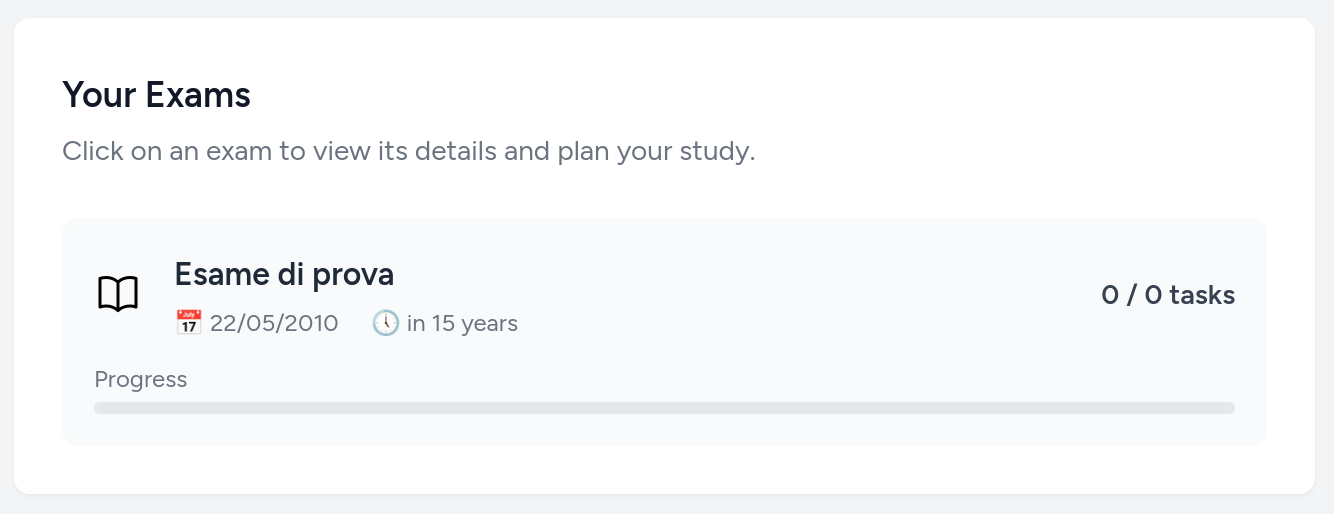
\includegraphics[width=6.5cm]{Screenshots/foglio4/Problema107.png}\hspace*{\fill}
    \vspace{10pt}
    \\
    \hline
    \textbf{Nome del valutatore} & Rinaldi \\
    \hline
  \end{tabular}
\end{table}

% Problema \getNumeroProblema
\begin{table}[htbp]
  \centering
  \renewcommand{\arraystretch}{1.5}
  \begin{tabular}{|>{\raggedright\arraybackslash}p{7.5cm}|>{\raggedright\arraybackslash}p{7.5cm}|}
    \hline
    \rowcolor{green!30}
    \multicolumn{2}{|c|}{\textbf{Problema \getNumeroProblema}} \\
    \hline
    \textbf{Descrizione} & Nella visualizzazione dei dettagli di un esame, cliccando il pulsante "Aggiungi materiale esistente", viene mostrato il messaggio "Tutti i tuoi documenti sono già stati collegati!" anche quando non sono presenti materiali nel proprio repository. \\
    \hline
    \textbf{Pagina del sito} & StudyFlow AI \\
    \hline
    \textbf{Principi violati} & 1 (Far vedere lo stato del sistema); 9 (Permettere all’utente di correggere gli errori e non solo di rilevarli) \\
    \hline
    \textbf{Grado di severità} & 2 (Problema secondario) \\
    \hline
    \textbf{Screen} &
    \vspace{10pt}
    \hspace*{\fill}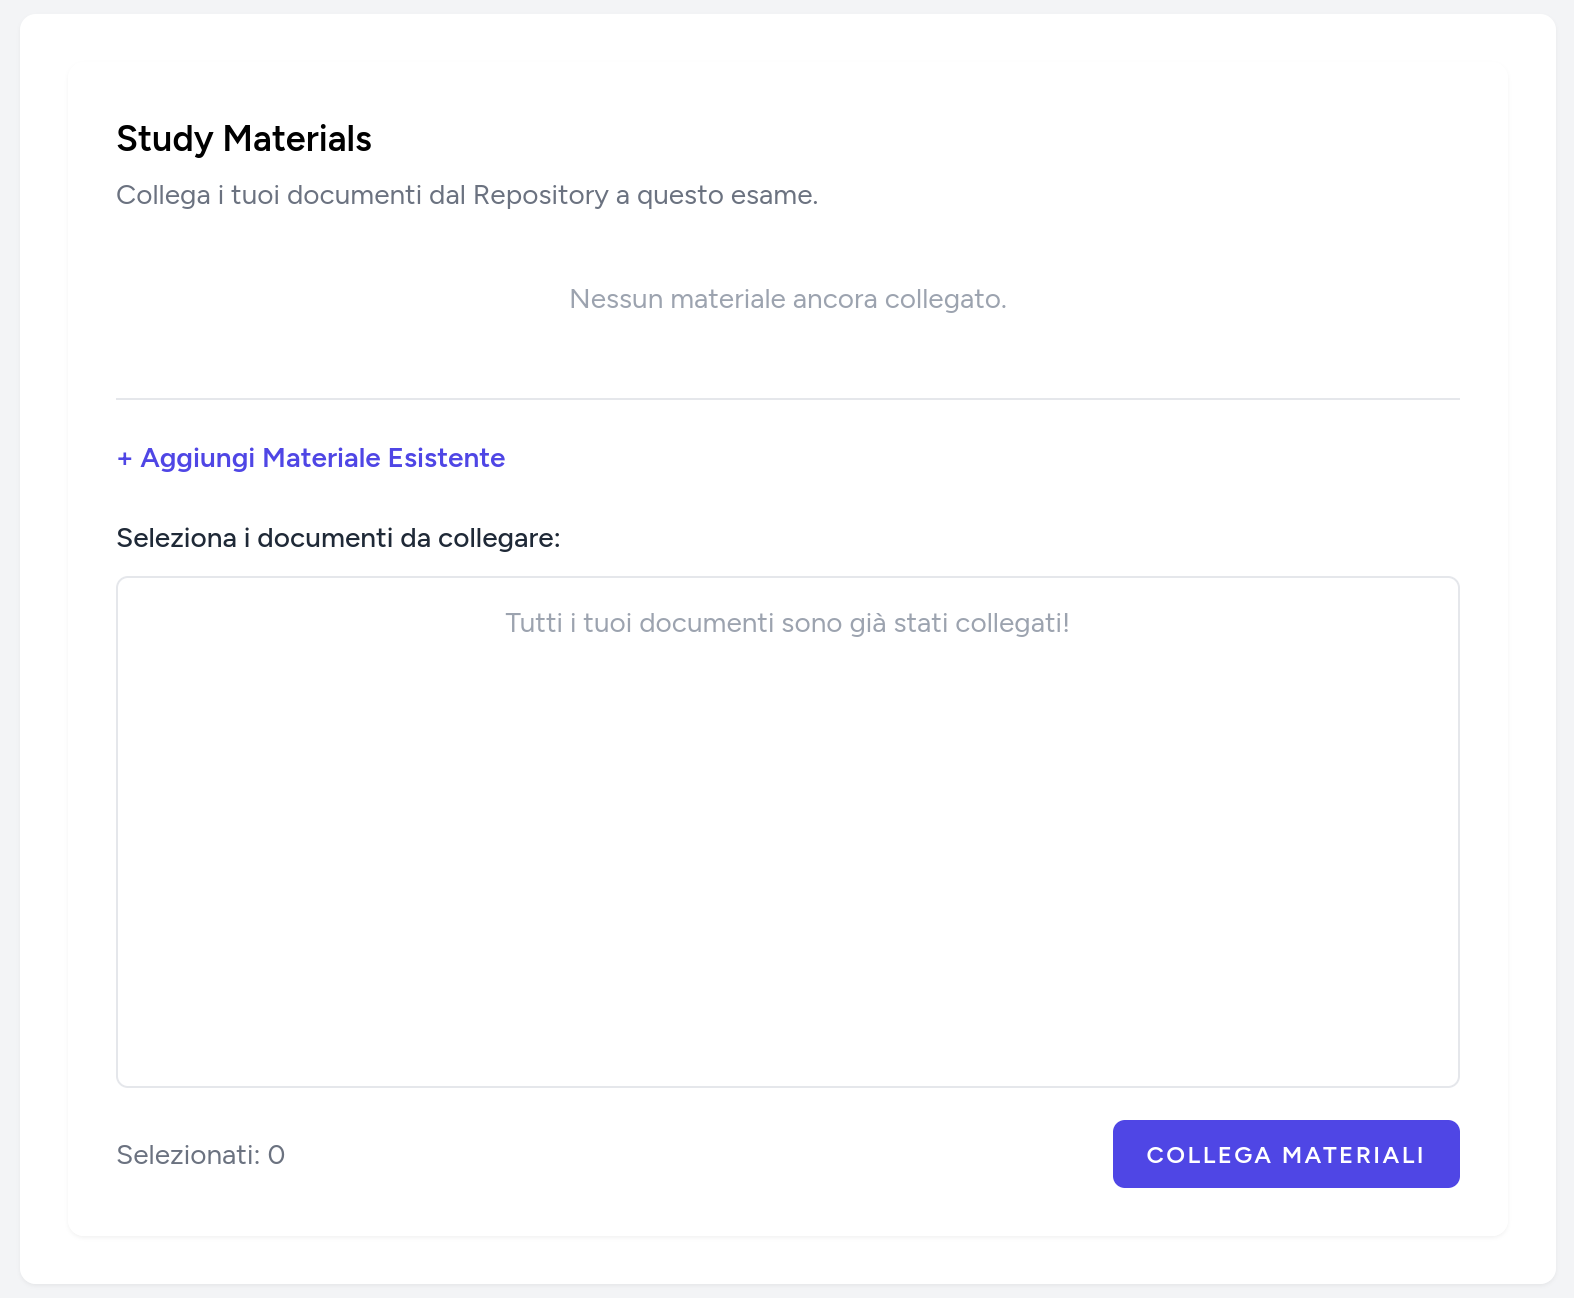
\includegraphics[width=6.5cm]{Screenshots/foglio4/Problema108.png}\hspace*{\fill}
    \vspace{10pt}
    \\
    \hline
    \textbf{Nome del valutatore} & Rinaldi \\
    \hline
  \end{tabular}
\end{table}

% Problema \getNumeroProblema
\begin{table}[htbp]
  \centering
  \renewcommand{\arraystretch}{1.5}
  \begin{tabular}{|>{\raggedright\arraybackslash}p{7.5cm}|>{\raggedright\arraybackslash}p{7.5cm}|}
    \hline
    \rowcolor{green!30}
    \multicolumn{2}{|c|}{\textbf{Problema \getNumeroProblema}} \\
    \hline
    \textbf{Descrizione} &  Nella visualizzazione dei dettagli di un esame, cliccando il pulsante "Aggiungi materiale esistente", quando non sono presenti materiali nel proprio repository, il pulsante "Collega materiali" compare senza alcuna funzione attiva. \\
    \hline
    \textbf{Pagina del sito} & StudyFlow AI \\
    \hline
    \textbf{Principi violati} & 7 (Visualizzare tutte e sole le informazioni necessarie) \\
    \hline
    \textbf{Grado di severità} & 1 (Problema accessorio) \\
    \hline
    \textbf{Screen} &
    \vspace{10pt}
    \hspace*{\fill}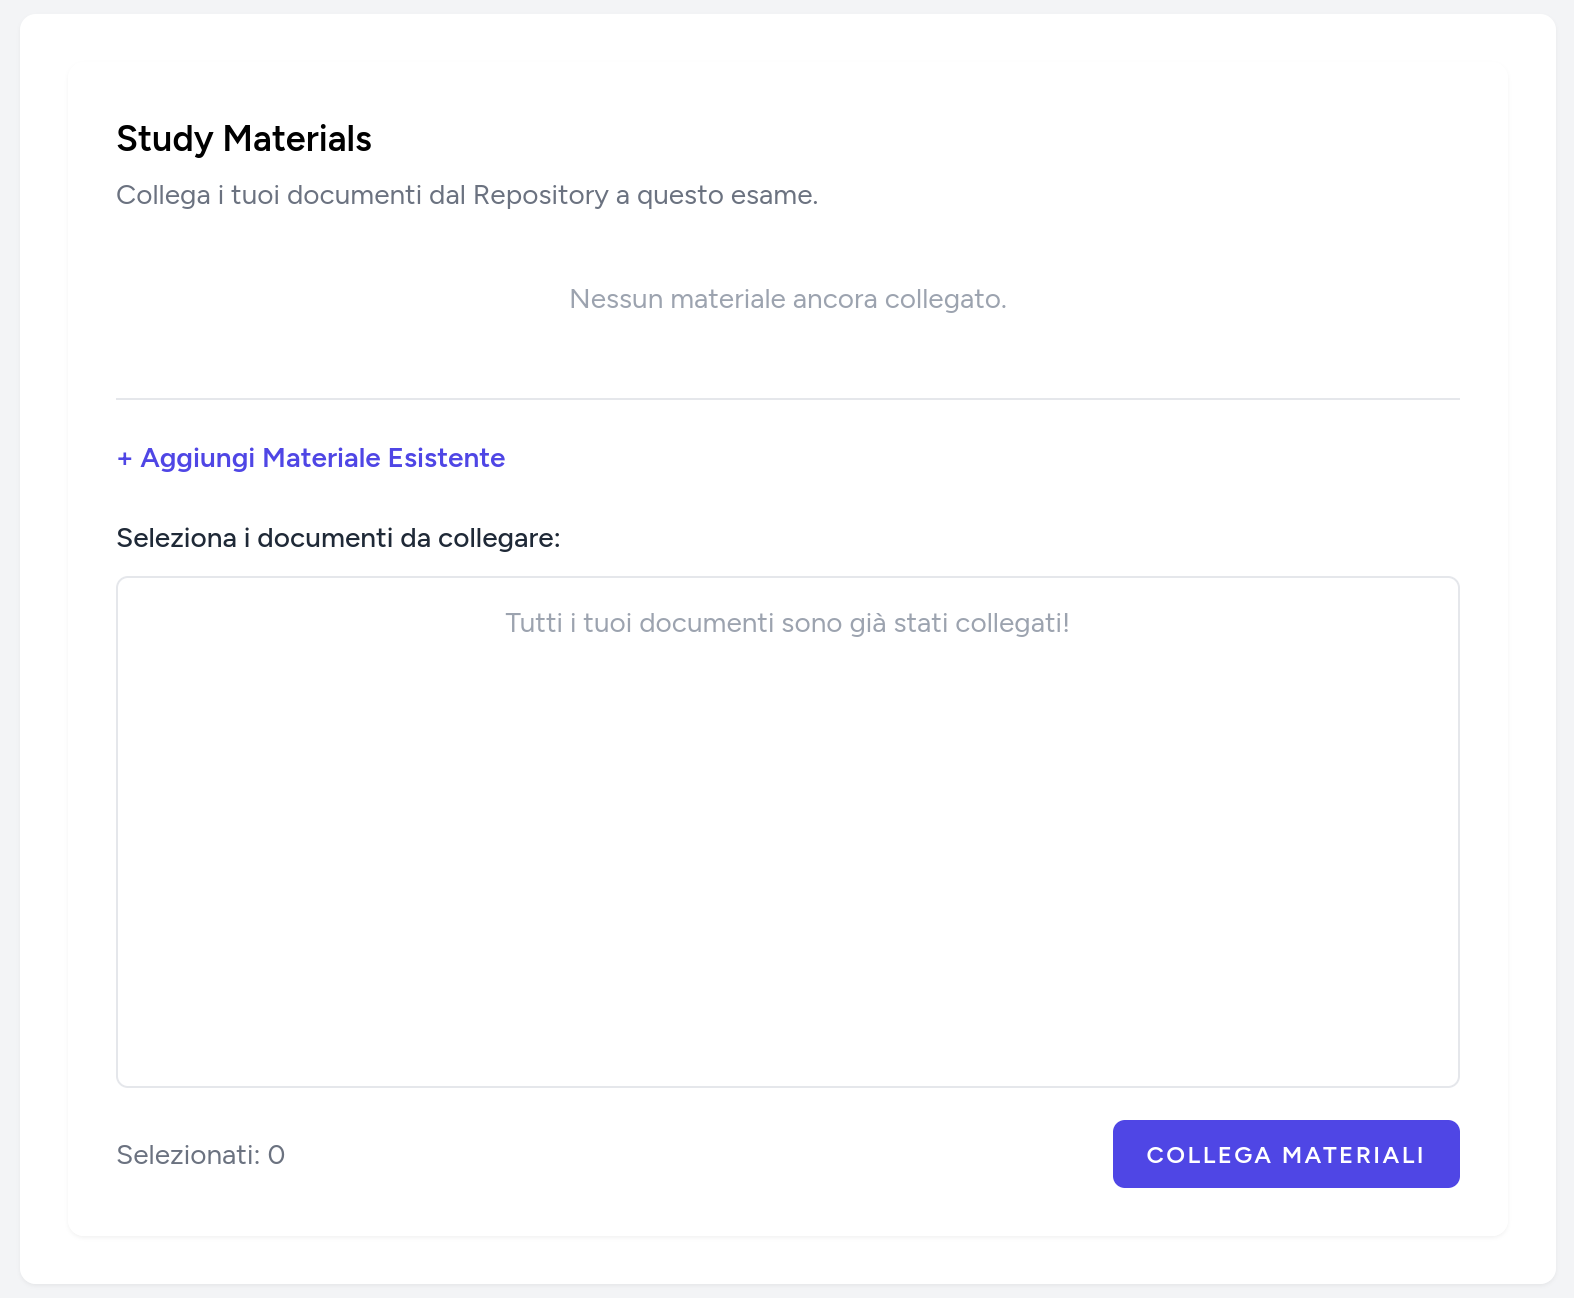
\includegraphics[width=6.5cm]{Screenshots/foglio4/Problema109.png}\hspace*{\fill}
    \vspace{10pt}
    \\
    \hline
    \textbf{Nome del valutatore} & Rinaldi \\
    \hline
  \end{tabular}
\end{table}

% Problema \getNumeroProblema
\begin{table}[htbp]
  \centering
  \renewcommand{\arraystretch}{1.5}
  \begin{tabular}{|>{\raggedright\arraybackslash}p{7.5cm}|>{\raggedright\arraybackslash}p{7.5cm}|}
    \hline
    \rowcolor{green!30}
    \multicolumn{2}{|c|}{\textbf{Problema \getNumeroProblema}} \\
    \hline
    \textbf{Descrizione} &  Nei dettagli di un esame se si elimina una task compare un avviso che può risultare "strano" all'utente in cui viene chiesto se si è sicuri di voler eliminare l'attività.\\
    \hline
    \textbf{Pagina del sito} & StudyFlow AI \\
    \hline
    \textbf{Principi violati} & 4 (Assicurare consistenza); 6 (Assicurare flessibilità ed efficienza d’uso ) \\
    \hline
    \textbf{Grado di severità} & 3 (Problema rilevante) \\
    \hline
    \textbf{Screen} &
    \vspace{10pt}
    \hspace*{\fill}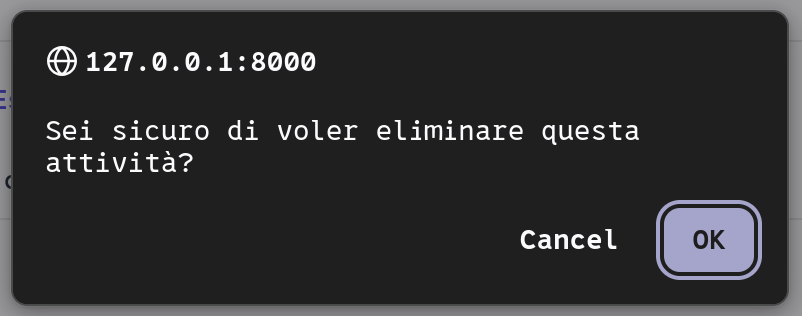
\includegraphics[width=6.5cm]{Screenshots/foglio4/Problema110.png}\hspace*{\fill}
    \vspace{10pt}
    \\
    \hline
    \textbf{Nome del valutatore} & Rinaldi \\
    \hline
  \end{tabular}
\end{table}

% Problema \getNumeroProblema
\begin{table}[htbp]
  \centering
  \renewcommand{\arraystretch}{1.5}
  \begin{tabular}{|>{\raggedright\arraybackslash}p{7.5cm}|>{\raggedright\arraybackslash}p{7.5cm}|}
    \hline
    \rowcolor{green!30}
    \multicolumn{2}{|c|}{\textbf{Problema \getNumeroProblema}} \\
    \hline
    \textbf{Descrizione} &  Nella sezione "Exam Details" è presente una sezione del calendario non funzionante. \\
    \hline
    \textbf{Pagina del sito} & StudyFlow AI \\
    \hline
    \textbf{Principi violati} & 4 (Assicurare consistenza) \\
    \hline
    \textbf{Grado di severità} & 4 (Catastrofe di usabilità) \\
    \hline
    \textbf{Screen} &
    \vspace{10pt}
    \hspace*{\fill}
\includegraphics[width=6.5cm]{Screenshots/foglio4/Problema111.png}\hspace*{\fill}
    \vspace{10pt}
    \\
    \hline
    \textbf{Nome del valutatore} & Rinaldi, Kharef \\
    \hline
  \end{tabular}
\end{table}


% Problema \getNumeroProblema
\begin{table}[htbp]
  \centering
  \renewcommand{\arraystretch}{1.5}
  \begin{tabular}{|>{\raggedright\arraybackslash}p{7.5cm}|>{\raggedright\arraybackslash}p{7.5cm}|}
    \hline
    \rowcolor{green!30}
    \multicolumn{2}{|c|}{\textbf{Problema \getNumeroProblema}} \\
    \hline
    \textbf{Descrizione} &   Durante il caricamento di un file è obbligatorio inserire tutti i dettagli del documento, anche se non si intende renderlo pubblico. \\
    \hline
    \textbf{Pagina del sito} & I Miei Appunti - Caricamento file \\
    \hline
    \textbf{Principi violati} & 6 (Assicurare flessibilità ed efficienza d'uso); 7 (Visualizzare tutte e sole le informazioni necessarie) \\
    \hline
    \textbf{Grado di severità} & 1 (Problema accessorio) \\
    \hline
    \textbf{Nome del valutatore} & Rinaldi \\
    \hline
  \end{tabular}
\end{table}

% Problema \getNumeroProblema
\begin{table}[htbp]
  \centering
  \renewcommand{\arraystretch}{1.5}
  \begin{tabular}{|>{\raggedright\arraybackslash}p{7.5cm}|>{\raggedright\arraybackslash}p{7.5cm}|}
    \hline
    \rowcolor{green!30}
    \multicolumn{2}{|c|}{\textbf{Problema \getNumeroProblema}} \\
    \hline
    \textbf{Descrizione} & La sezione "Your Exams" è accessibile tramite il pulsante "StudyFlow AI", collocato nella sezione "Strumenti AI", il che risulta poco pertinente rispetto alla sua funzione. \\
    \hline
    \textbf{Pagina del sito} & StudyFlow AI\\
    \hline
    \textbf{Principi violati} & 4 (Assicurare consistenza) \\
    \hline
    \textbf{Grado di severità} & 1 (Problema accessorio) \\
    \hline
    \textbf{Screen} &
    \vspace{10pt}
    \hspace*{\fill}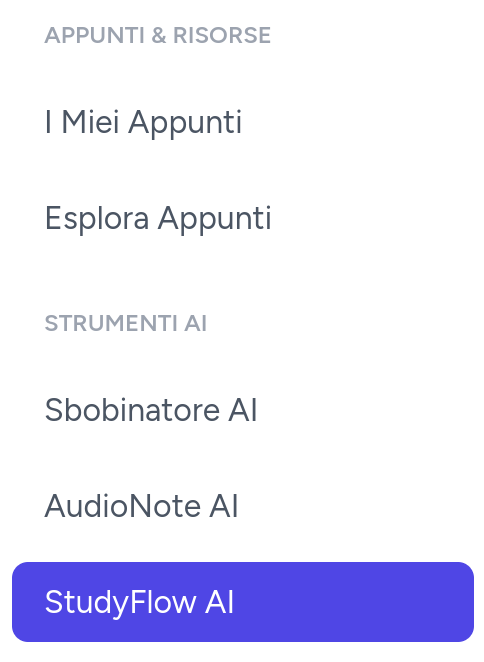
\includegraphics[width=6.5cm]{Screenshots/foglio4/Problema113.png}\hspace*{\fill}
    \vspace{10pt}
    \\
    \hline
    \textbf{Nome del valutatore} & Rinaldi \\
    \hline
  \end{tabular}
\end{table}

% Problema \getNumeroProblema
\begin{table}[htbp]
  \centering
  \renewcommand{\arraystretch}{1.5}
  \begin{tabular}{|>{\raggedright\arraybackslash}p{7.5cm}|>{\raggedright\arraybackslash}p{7.5cm}|}
    \hline
    \rowcolor{green!30}
    \multicolumn{2}{|c|}{\textbf{Problema \getNumeroProblema}} \\
    \hline
    \textbf{Descrizione} & In "Your Exams" non c'è la possibilità di eliminare un esame, ma solo di crearne di nuovi e aggiungerli alla lista. \\
    \hline
    \textbf{Pagina del sito} & StudyFlow AI \\
    \hline
    \textbf{Principi violati} & 2 (Adeguare il sistema al mondo reale); 3 (Controllo dell’utente e libertà); 9 (Permettere all’utente di correggere gli errori e non solo di rilevarli) \\
    \hline
    \textbf{Grado di severità} & 3 (Problema rilevante) \\
    \hline
    \textbf{Nome del valutatore} & Rinaldi \\
    \hline
  \end{tabular}
\end{table}

% Problema \getNumeroProblema
\begin{table}[htbp]
  \centering
  \renewcommand{\arraystretch}{1.5}
  \begin{tabular}{|>{\raggedright\arraybackslash}p{7.5cm}|>{\raggedright\arraybackslash}p{7.5cm}|}
    \hline
    \rowcolor{green!30}
    \multicolumn{2}{|c|}{\textbf{Problema \getNumeroProblema}} \\
    \hline
    \textbf{Descrizione} & Durante l'upload di un file vengono richiesti dettagli come università e dipartimento tramite menu a tendina che consentono di selezionare la voce "Seleziona . . ." che non dovrebbe essere selezionabile. \\
    \hline
    \textbf{Pagina del sito} & I Miei Appunti - Caricamento File \\
    \hline
    \textbf{Principi violati} & 7 (Visualizzare tutte e sole le informazioni necessarie); 8 (Prevenire gli errori) \\
    \hline
    \textbf{Grado di severità} & 2 (Problema secondario) \\
    \hline
    \textbf{Screen} &
    \vspace{10pt}
    \hspace*{\fill}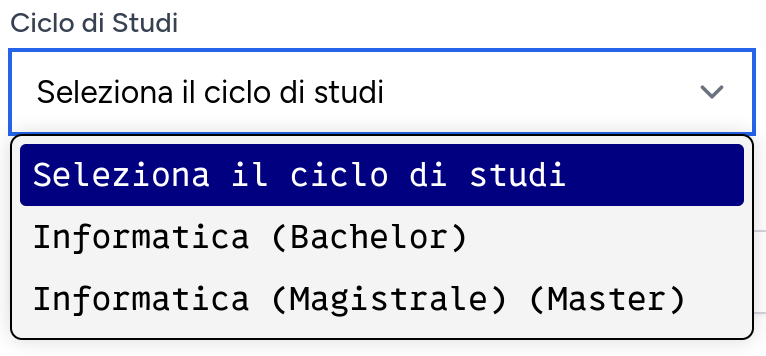
\includegraphics[width=6.5cm]{Screenshots/foglio4/Problema115.png}\hspace*{\fill}
    \vspace{10pt}
    \\
    \hline
    \textbf{Nome del valutatore} & Rinaldi \\
    \hline
  \end{tabular}
\end{table}

% Problema \getNumeroProblema
\begin{table}[htbp]
  \centering
  \renewcommand{\arraystretch}{1.5}
  \begin{tabular}{|>{\raggedright\arraybackslash}p{7.5cm}|>{\raggedright\arraybackslash}p{7.5cm}|}
    \hline
    \rowcolor{green!30}
    \multicolumn{2}{|c|}{\textbf{Problema \getNumeroProblema}} \\
    \hline
    \textbf{Descrizione} & Durante l'upload di un file vengono richiesti dettagli come università e dipartimento tramite menu a tendina e, in alcuni casi, la mancata selezione non genera alcun messaggio/avviso di errore al momento del click del pulsante di salvataggio. \\
    \hline
    \textbf{Pagina del sito} & I Miei Appunti - Caricamento File \\
    \hline
    \textbf{Principi violati} & 1 (Far vedere lo stato del sistema); 8 (Prevenire gli errori); 9 (Permettere all'utente di correggere gli errori e non solo di rilevarli) \\
    \hline
    \textbf{Grado di severità} & 3 (Problema rilevante) \\
    \hline
    \textbf{Screen} &
    \vspace{10pt}
    \hspace*{\fill}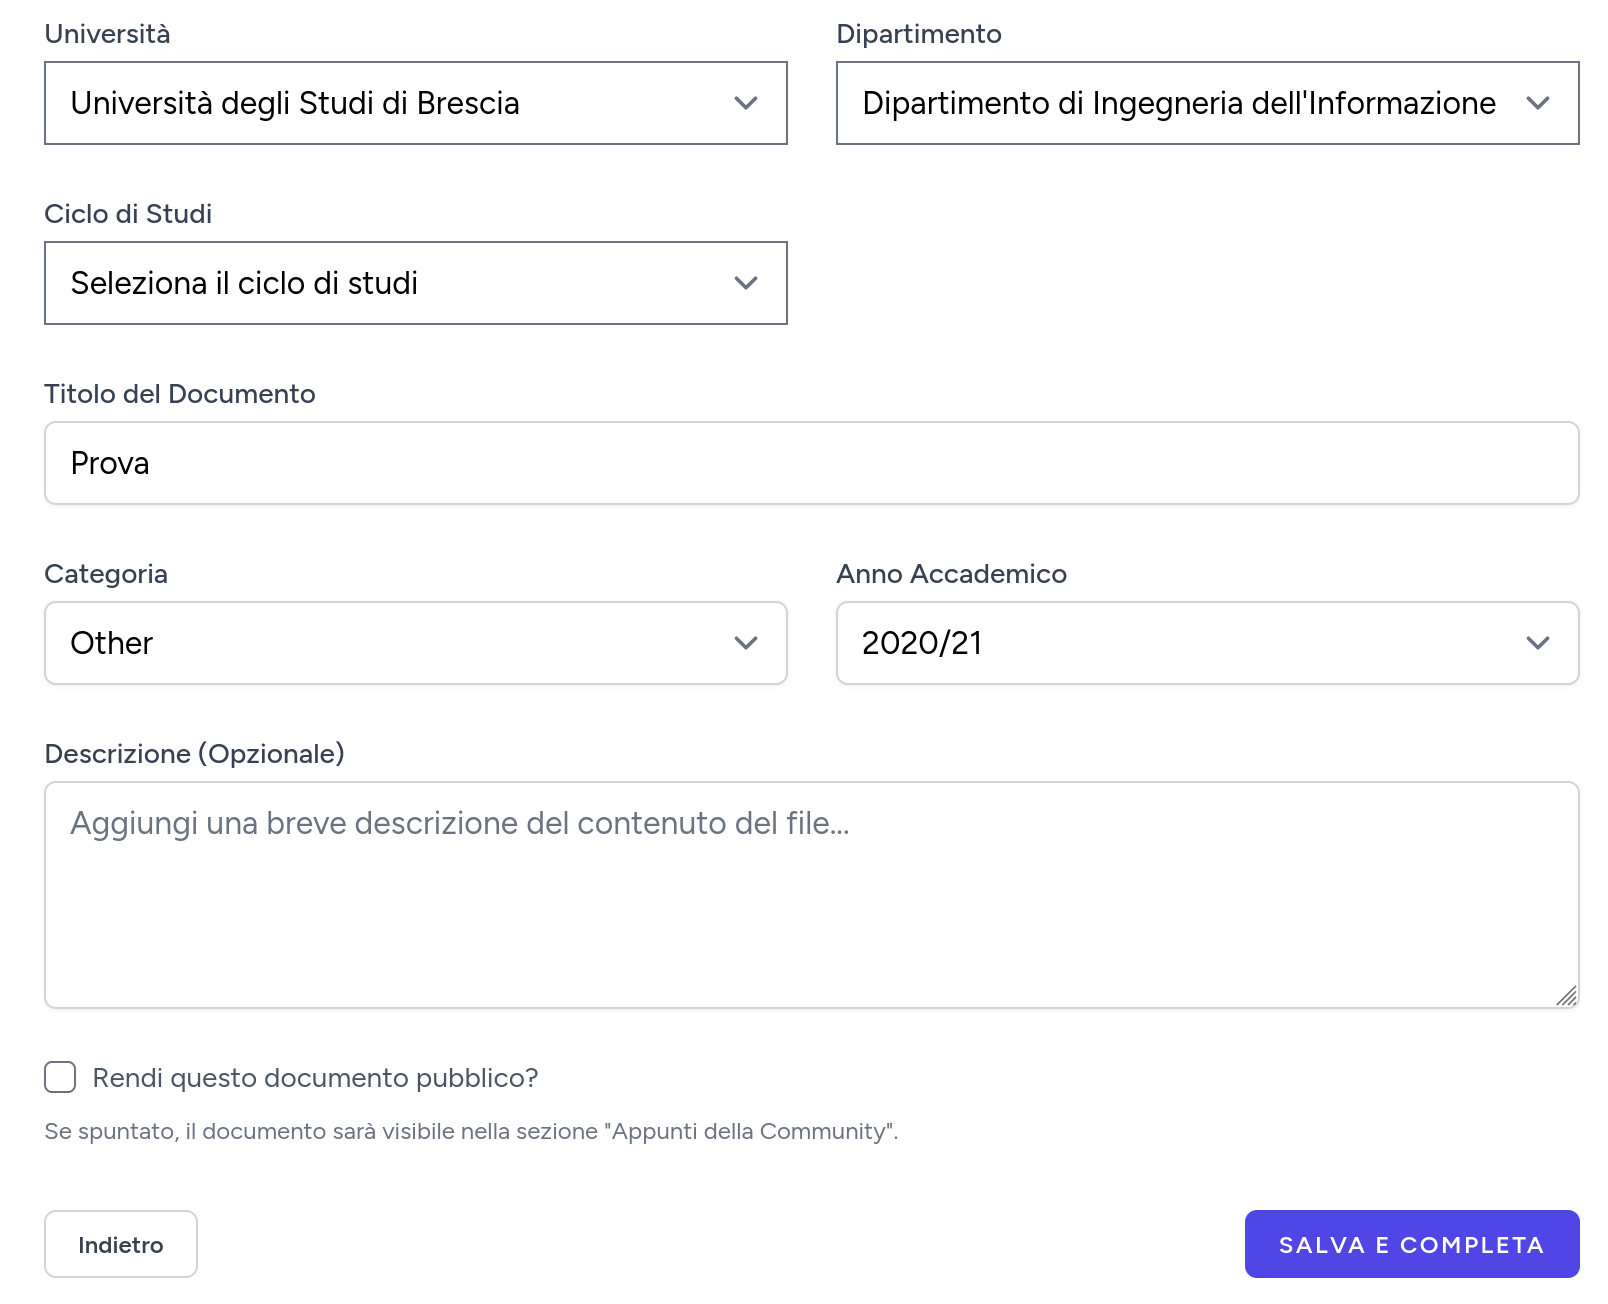
\includegraphics[width=6.5cm]{Screenshots/foglio4/Problema116.png}\hspace*{\fill}
    \vspace{10pt}
    \\
    \hline
    \textbf{Nome del valutatore} & Rinaldi \\
    \hline
  \end{tabular}
\end{table}

\FloatBarrier

\subsubsection{Classificazione dei problemi individuati}
Ogni problema è stato valutato assegnando un grado di severità da 0 a 4:
\begin{itemize}
  \item 0: Non è un problema di usabilità
  \item 1: Problema accessorio
  \item 2: Problema secondario
  \item 3: Problema rilevante
  \item 4: Catastrofe di usabilità
\end{itemize}
Nel grafico seguente è riportata la distribuzione dei problemi per grado di severità:
\begin{figure}[H]
  \centering
  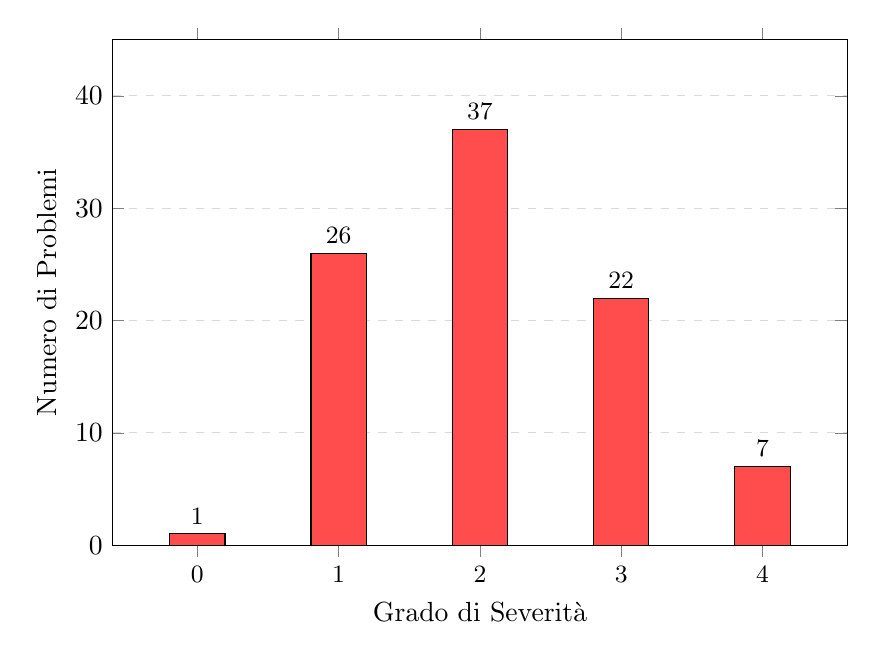
\begin{tikzpicture}
    \begin{axis}[
        ybar,
        bar width=20pt,
        width=0.9\textwidth,
        height=8cm,
        symbolic x coords={S0, S1, S2, S3, S4},
        xtick=data,
        xticklabels={0, 1, 2, 3, 4},
        x tick label style={font=\small},
        xlabel={Grado di Severità},
        ylabel={Numero di Problemi},
        ymin=0,
        ymax=45,
        ymajorgrids=true,
        grid style={dashed, gray!30},
        enlarge x limits=0.15,
        nodes near coords,
        every node near coord/.style={font=\small, color=black},
      ]
      \addplot+[ybar, fill=red!70, draw=black] coordinates {
        (S0,1)
        (S1,26)
        (S2,37)
        (S3,22)
        (S4,7)
      };
    \end{axis}
  \end{tikzpicture}
  \label{fig:severita-problemi}
  \caption{Classificazione dei problemi riscontrati rispetto al grado di severità assegnato.}
\end{figure}

La maggior parte dei problemi identificati (37 su 93, pari a circa il 40\%) rientra nella categoria di severità 2 (problemi secondari), seguita dai problemi accessori di 
severità 1 (26, pari a circa il 28\%). I problemi di severità 3 e 4, che richiedono interventi prioritari, rappresentano complessivamente circa il 31\% del totale (29 problemi). 

La distribuzione suggerisce che il sistema presenta principalmente problematiche di entità moderata, ma non mancano criticità rilevanti che dovranno essere affrontate nelle fasi successive di sviluppo.

\subsubsection{Distribuzione dei problemi per numero di valutatori}
Per ogni problema è stata analizzata la distribuzione rispetto al numero di valutatori che lo hanno individuato. Le tabelle seguenti mostrano, per ciascun valutatore, se il problema è stato rilevato o meno.
\vspace{0.3cm}

% Tabella 1: Problemi 1-15
\begin{figure}[H]
\centering
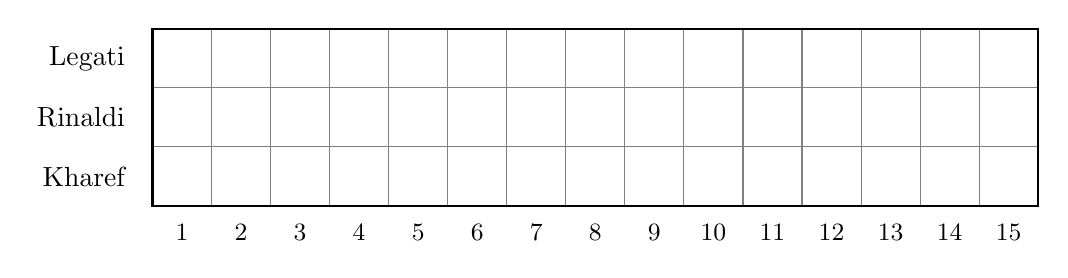
\begin{tikzpicture}[scale=0.75]
    \definecolor{checkcolor}{RGB}{0,0,0}
    
    %\node[anchor=south, font=\large] at (8.5, 4.2) {Problemi 1-15};
    
    % Etichette asse Y
    \node[anchor=east, font=\normalsize] at (0.7, 3.5) {Legati};
    \node[anchor=east, font=\normalsize] at (0.7, 2.5) {Rinaldi};
    \node[anchor=east, font=\normalsize] at (0.7, 1.5) {Kharef};
    
    % Etichette asse X
    \foreach \x in {1,...,15} {
        \node[font=\small] at (\x+0.5, 0.55) {\x};
    }
    
    % Griglia
    \draw[gray!100] (1, 1) grid[step=1] (16, 4);
    \draw[black, thick] (1, 1) rectangle (16, 4);
    
    % Riempimento di default: metto la X rossa ovunque
    \foreach \x in {1,...,15} {
        \node at (\x+0.5, 3.5) {\notfound}; % Riga Legati
        \node at (\x+0.5, 2.5) {\notfound}; % Riga Rinaldi
        \node at (\x+0.5, 1.5) {\notfound}; % Riga Kharef
    }
    
    % Sovrascrivo con la spunta verde DOVE HANNO TROVATO il problema
    
    % Dati - Legati (Trovati)
    \foreach \x in {1,2,3,4,5,6,7,8,9,10,11,12,13,14,15} {
        \node[fill=white, inner sep=1pt] at (\x+0.5, 3.5) {\found};
    }
    
    % Dati - Rinaldi (Trovati)
    \foreach \x in {2,3,5,6,8,9,11,12,13,14} {
        \node[fill=white, inner sep=1pt] at (\x+0.5, 2.5) {\found};
    }
    
    % Dati - Kharef (Trovati)
    \foreach \x in {2,3,5,6,9,11,12,15} {
        \node[fill=white, inner sep=1pt] at (\x+0.5, 1.5) {\found};
    }
\end{tikzpicture}
\end{figure}

% Tabella 2: Problemi 16-30
\begin{figure}[H]
\centering
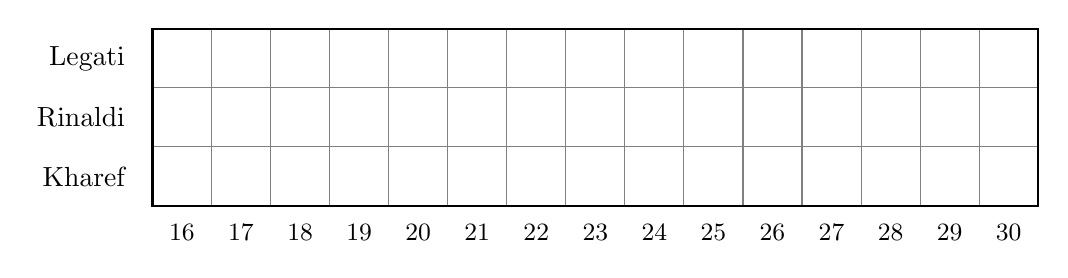
\begin{tikzpicture}[scale=0.75]
    \definecolor{checkcolor}{RGB}{0,0,0}
    
    % Etichette asse Y
    \node[anchor=east, font=\normalsize] at (0.7, 3.5) {Legati};
    \node[anchor=east, font=\normalsize] at (0.7, 2.5) {Rinaldi};
    \node[anchor=east, font=\normalsize] at (0.7, 1.5) {Kharef};
    
    % Etichette asse X
    \foreach \x/\label in {1/16,2/17,3/18,4/19,5/20,6/21,7/22,8/23,9/24,10/25,11/26,12/27,13/28,14/29,15/30} {
        \node[font=\small] at (\x+0.5, 0.55) {\label};
    }
    
    % Griglia
    \draw[gray!100] (1, 1) grid[step=1] (16, 4);
    \draw[black, thick] (1, 1) rectangle (16, 4);
    
    % Default: X rossa
    \foreach \x in {1,...,15} {
        \node at (\x+0.5, 3.5) {\notfound};
        \node at (\x+0.5, 2.5) {\notfound};
        \node at (\x+0.5, 1.5) {\notfound};
    }
    
    % Dati - Legati (Trovati)
    \foreach \x in {2,6,7,8,9,10,11,12,13,14,15} {
        \node[fill=white, inner sep=1pt] at (\x+0.5, 3.5) {\found};
    }
    
    % Dati - Rinaldi (Trovati)
    \foreach \x in {1,2,3,4,6,11,13} {
        \node[fill=white, inner sep=1pt] at (\x+0.5, 2.5) {\found};
    }
    
    % Dati - Kharef (Trovati)
    \foreach \x in {2,6,13} {
        \node[fill=white, inner sep=1pt] at (\x+0.5, 1.5) {\found};
    }
\end{tikzpicture}
\end{figure}

% Tabella 3: Problemi 31-45
\begin{figure}[H]
\centering
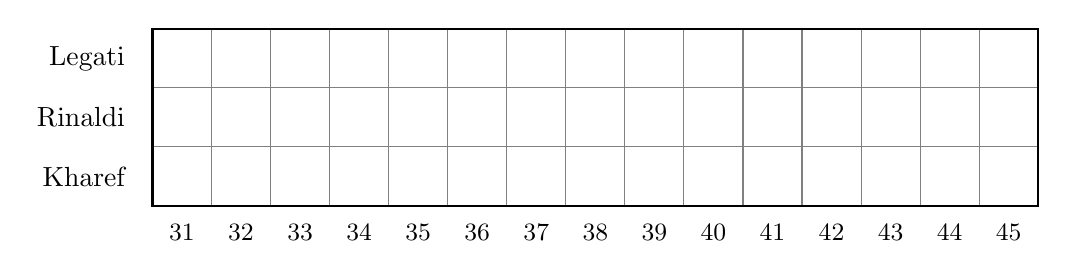
\begin{tikzpicture}[scale=0.75]
    \definecolor{checkcolor}{RGB}{0,0,0}
    
    % Etichette asse Y
    \node[anchor=east, font=\normalsize] at (0.7, 3.5) {Legati};
    \node[anchor=east, font=\normalsize] at (0.7, 2.5) {Rinaldi};
    \node[anchor=east, font=\normalsize] at (0.7, 1.5) {Kharef};
    
    % Etichette asse X
    \foreach \x/\label in {1/31,2/32,3/33,4/34,5/35,6/36,7/37,8/38,9/39,10/40,11/41,12/42,13/43,14/44,15/45} {
        \node[font=\small] at (\x+0.5, 0.55) {\label};
    }
    
    % Griglia
    \draw[gray!100] (1, 1) grid[step=1] (16, 4);
    \draw[black, thick] (1, 1) rectangle (16, 4);
    
    % Default: X rossa
    \foreach \x in {1,...,15} {
        \node at (\x+0.5, 3.5) {\notfound};
        \node at (\x+0.5, 2.5) {\notfound};
        \node at (\x+0.5, 1.5) {\notfound};
    }
    
    % Dati - Legati (Trovati)
    \foreach \x in {1,2,3,4,5,6,7,8,9,10,11,12,13,14,15} {
        \node[fill=white, inner sep=1pt] at (\x+0.5, 3.5) {\found};
    }
    
    % Dati - Rinaldi (Trovati)
    \foreach \x in {3,5,8,10} {
        \node[fill=white, inner sep=1pt] at (\x+0.5, 2.5) {\found};
    }
    
    % Dati - Kharef (Trovati)
    \foreach \x in {5,7,11,13,15} {
        \node[fill=white, inner sep=1pt] at (\x+0.5, 1.5) {\found};
    }
\end{tikzpicture}
\end{figure}

% Tabella 4: Problemi 46-60
\begin{figure}[H]
\centering
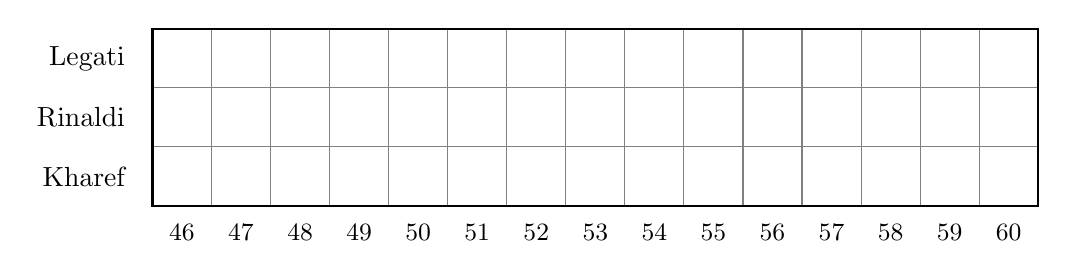
\begin{tikzpicture}[scale=0.75]
    \definecolor{checkcolor}{RGB}{0,0,0}
    
    % Etichette asse Y
    \node[anchor=east, font=\normalsize] at (0.7, 3.5) {Legati};
    \node[anchor=east, font=\normalsize] at (0.7, 2.5) {Rinaldi};
    \node[anchor=east, font=\normalsize] at (0.7, 1.5) {Kharef};
    
    % Etichette asse X
    \foreach \x/\label in {1/46,2/47,3/48,4/49,5/50,6/51,7/52,8/53,9/54,10/55,11/56,12/57,13/58,14/59,15/60} {
        \node[font=\small] at (\x+0.5, 0.55) {\label};
    }
    
    % Griglia
    \draw[gray!100] (1, 1) grid[step=1] (16, 4);
    \draw[black, thick] (1, 1) rectangle (16, 4);
    
    % Default: X rossa
    \foreach \x in {1,...,15} {
        \node at (\x+0.5, 3.5) {\notfound};
        \node at (\x+0.5, 2.5) {\notfound};
        \node at (\x+0.5, 1.5) {\notfound};
    }
    
    % Dati - Legati (Trovati)
    \foreach \x in {1,2,3} {
        \node[fill=white, inner sep=1pt] at (\x+0.5, 3.5) {\found};
    }
    
    % Dati - Rinaldi (Trovati)
    \foreach \x in {3} {
        \node[fill=white, inner sep=1pt] at (\x+0.5, 2.5) {\found};
    }
    
    % Dati - Kharef (Trovati)
    \foreach \x in {4,5,6,7,8,9,10,11,12,13,14,15} {
        \node[fill=white, inner sep=1pt] at (\x+0.5, 1.5) {\found};
    }
\end{tikzpicture}
\end{figure}

% Tabella 5: Problemi 61-75
\begin{figure}[H]
\centering
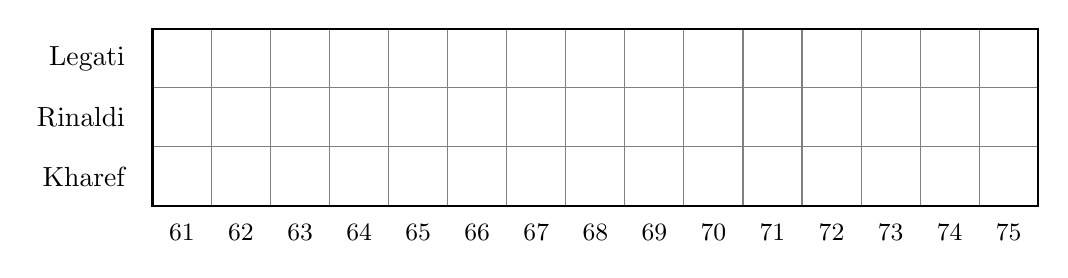
\begin{tikzpicture}[scale=0.75]
    \definecolor{checkcolor}{RGB}{0,0,0}
    
    % Etichette asse Y
    \node[anchor=east, font=\normalsize] at (0.7, 3.5) {Legati};
    \node[anchor=east, font=\normalsize] at (0.7, 2.5) {Rinaldi};
    \node[anchor=east, font=\normalsize] at (0.7, 1.5) {Kharef};
    
    % Etichette asse X
    \foreach \x/\label in {1/61,2/62,3/63,4/64,5/65,6/66,7/67,8/68,9/69,10/70,11/71,12/72,13/73,14/74,15/75} {
        \node[font=\small] at (\x+0.5, 0.55) {\label};
    }
    
    % Griglia
    \draw[gray!100] (1, 1) grid[step=1] (16, 4);
    \draw[black, thick] (1, 1) rectangle (16, 4);
    
    % Default: X rossa
    \foreach \x in {1,...,15} {
        \node at (\x+0.5, 3.5) {\notfound};
        \node at (\x+0.5, 2.5) {\notfound};
        \node at (\x+0.5, 1.5) {\notfound};
    }
    
    % Dati - Kharef (Trovati) - Gli altri due valutatori qui hanno tutte X rosse
    \foreach \x in {1,2,3,4,5,6,7,8,9,10,11,12,13,14,15} {
        \node[fill=white, inner sep=1pt] at (\x+0.5, 1.5) {\found};
    }
\end{tikzpicture}
\end{figure}

% Tabella 6: Problemi 76-93
\begin{figure}[H]
\centering
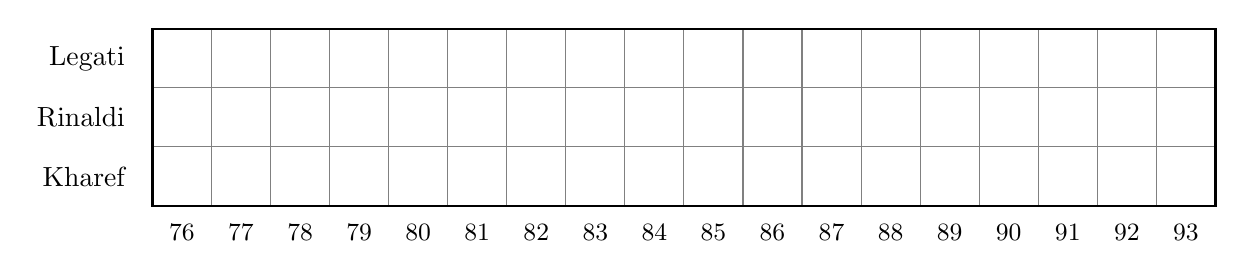
\begin{tikzpicture}[scale=0.75]
    \definecolor{checkcolor}{RGB}{0,0,0}
    
    % Etichette asse Y
    \node[anchor=east, font=\normalsize] at (0.7, 3.5) {Legati};
    \node[anchor=east, font=\normalsize] at (0.7, 2.5) {Rinaldi};
    \node[anchor=east, font=\normalsize] at (0.7, 1.5) {Kharef};
    
    % Etichette asse X
    \foreach \x/\label in {1/76,2/77,3/78,4/79,5/80,6/81,7/82,8/83,9/84,10/85,11/86,12/87,13/88,14/89,15/90,16/91,17/92,18/93} {
        \node[font=\small] at (\x+0.5, 0.55) {\label};
    }
    
    % Griglia
    \draw[gray!100] (1, 1) grid[step=1] (19, 4);
    \draw[black, thick] (1, 1) rectangle (19, 4);
    
    % Default: X rossa
    \foreach \x in {1,...,18} {
        \node at (\x+0.5, 3.5) {\notfound};
        \node at (\x+0.5, 2.5) {\notfound};
        \node at (\x+0.5, 1.5) {\notfound};
    }
    
    % Dati - Rinaldi (Trovati)
    \foreach \x in {5,6,7,8,9,10,11,12,13,14,15,16,17,18} {
        \node[fill=white, inner sep=1pt] at (\x+0.5, 2.5) {\found};
    }
    
    % Dati - Kharef (Trovati)
    \foreach \x in {1,2,3,4,12} {
        \node[fill=white, inner sep=1pt] at (\x+0.5, 1.5) {\found};
    }
\end{tikzpicture}
\end{figure}

\noindent
Sui 93 problemi totali individuati, di cui alcuni sono stati rilevati da più valutatori, la tabella seguente riporta un riepilogo del contributo di ciascun valutatore con le relative percentuali.
% Tabella Riepilogo
\begin{center}
    \renewcommand{\arraystretch}{1.3}
    \begin{tabular}{|l|c|c|}
        \hline
        \textbf{Valutatore} & \textbf{Problemi Identificati} & \textbf{Percentuale} \\
        \hline
        Legati & 44 & $47\%$ \\
        \hline
        Rinaldi & 36 & $38\%$ \\
        \hline
        Kharef & 48 & $52\%$ \\
        \hline
    \end{tabular}
\end{center}

\vspace{0.3cm}

Dall'analisi dei risultati emerge una certa variabilità nel numero di problemi individuati dai diversi valutatori. Si nota in particolare che Kharef ha rilevato più criticità rispetto alla media del gruppo (52\% contro una media del 45\%). 

Questo risultato può essere attribuito al fatto che, avendo sviluppato il sistema, possedeva una conoscenza più approfondita dell'architettura e delle funzionalità di \textit{BrainBox}.

I valutatori hanno identificato in gran parte problemi diversi, con poche sovrapposizioni. 
Questo dimostra l'importanza di utilizzare valutatori con diversi gradi di familiarità 
con il sistema per una valutazione più completa.

\subsubsection{Confronto con la curva di Nielsen}
Per stimare la percentuale di problemi individuati da tre valutatori è stato fatto riferimento alla \textit{curva di Nielsen} (Figura \ref{curva_nielsen}), che modella la probabilità cumulativa di rilevazione dei problemi in funzione del numero di valutatori coinvolti. 

Assumendo che la probabilità che un singolo valutatore identifichi un problema sia pari a $L = 0.31$, la probabilità che almeno uno dei tre valutatori rilevi un determinato problema è:
\[
  1 - (1 - L)^3 = 1 - (1 - 0.31)^3 \approx 0.672
\]

ossia circa il 67.2\% dei problemi effettivamente presenti. Secondo il modello di Nielsen, ci si aspetta quindi che tre valutatori siano in grado di individuare complessivamente il 67.2\% dei problemi dell'interfaccia.

A partire da questa stima, si può ricavare il numero totale di problemi presenti. Indicando con $P$ il numero di problemi rilevati e con $N$ il numero totale di problemi esistenti, si ha:
\[
  P : N = 67.2 : 100
\]

\noindent
Poiché i tre valutatori hanno identificato $P = 93$ problemi unici, si ottiene:
\[
  93 : N = 67.2 : 100
\]

\noindent
Da cui segue:
\[
  N = \frac{93 \times 100}{67.2} \approx 138
\]

\noindent
Pertanto, il \textit{numero totale di problemi stimati} nell'interfaccia risulta essere circa 138.

\begin{figure}[H]
  \centering
  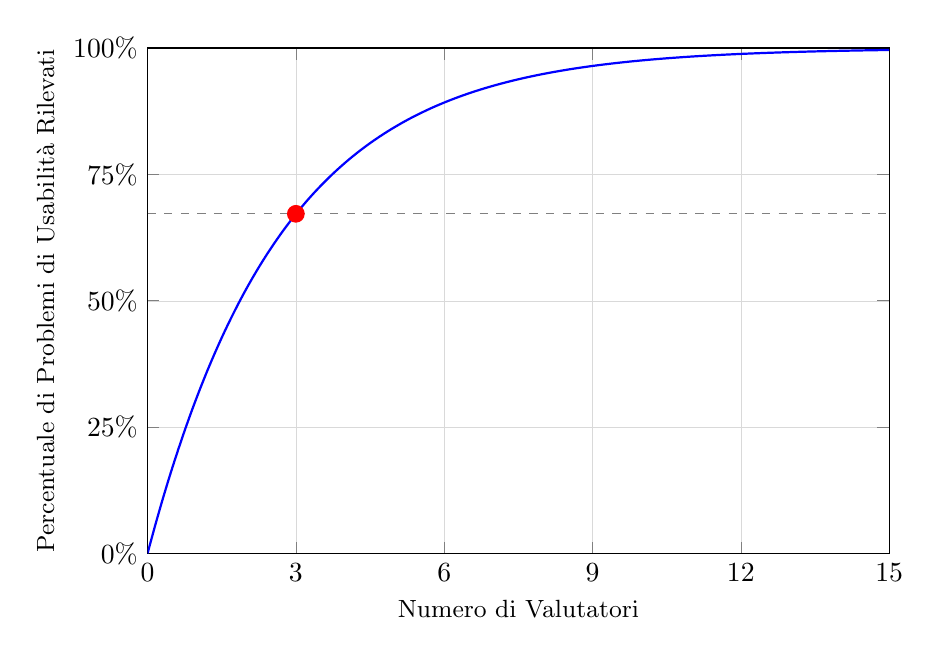
\begin{tikzpicture}
    \begin{axis}[
        width=11cm,
        height=8cm,
        xlabel={Numero di Valutatori},
        ylabel={Percentuale di Problemi di Usabilità Rilevati},
        xmin=0, xmax=15,
        ymin=0, ymax=100,
        xtick={0,3,6,9,12,15},
        ytick={0,25,50,75,100},
        yticklabels={0\%,25\%,50\%,75\%,100\%},
        grid=major,
        grid style={line width=.1pt, draw=gray!30},
        xlabel style={font=\small},
        ylabel style={font=\small, align=center},
      ]

      % Curva di Nielsen (L=0.31)
      \addplot[domain=0:15, samples=100, smooth, thick, blue]
      {100*(1 - (1-0.31)^x)};

      % Linea tratteggiata orizzontale al 67.2%
      \addplot[dashed, gray, thin] coordinates {(0,67.2) (15,67.2)};

      % Punto per 3 valutatori
      \addplot[mark=*, mark size=3pt, red, only marks]
      coordinates {(3, 67.2)};

    \end{axis}
  \end{tikzpicture}
  \caption{Curva di Nielsen.}
  \label{curva_nielsen}
\end{figure}

\subsubsection{Frequenza delle violazioni}
In questa sezione viene presentata l'analisi quantitativa dei problemi riscontrati durante la valutazione euristica. Al fine di fornire una panoramica chiara e strutturata delle principali criticità dell'interfaccia, i dati raccolti sono stati esaminati seguendo un approccio articolato su tre livelli. 

In primo luogo, i problemi sono stati classificati in base ai 10 principi euristici di Nielsen, permettendo così di identificare le regole specifiche di usabilità maggiormente violate (Figura \ref{fig:violazioni-nielsen}). Successivamente, per comprendere più a fondo la natura delle problematiche riscontrate, le medesime violazioni sono state aggregate in tre macro-categorie: \textit{percezione}, \textit{cognizione} ed \textit{errori} (Figura \ref{fig:categorie-principi-nielsen}). Infine, l'analisi si è concentrata sulla localizzazione delle criticità, mappandone la distribuzione all'interno delle diverse sezioni del sito (Figura \ref{fig:violazioni-sezioni-sito}).

Di seguito, si riporta la classificazione relativa ai singoli principi euristici di Nielsen.

\begin{figure}[H]
  \centering
  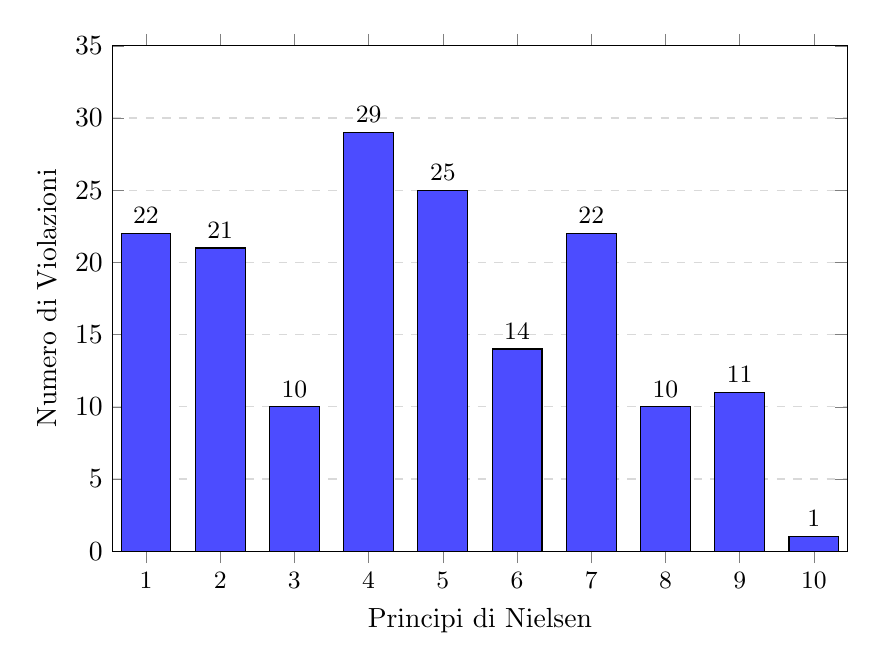
\begin{tikzpicture}
    \begin{axis}[
        ybar,
        bar width=18pt,
        width=0.9\textwidth,
        height=8cm,
        symbolic x coords={P1, P2, P3, P4, P5, P6, P7, P8, P9, P10},
        xtick=data,
        xticklabels={1, 2, 3, 4, 5, 6, 7, 8, 9, 10},
        x tick label style={font=\small},
        xlabel={Principi di Nielsen},
        ylabel={Numero di Violazioni},
        ymin=0,
        ymax=35,
        ymajorgrids=true,
        grid style={dashed, gray!30},
        enlarge x limits=0.05,
        nodes near coords,
        every node near coord/.style={font=\small, color=black},
      ]
      \addplot+[ybar, fill=blue!70, draw=black] coordinates {
        (P1,22)
        (P2,21)
        (P3,10)
        (P4,29)
        (P5,25)
        (P6,14)
        (P7,22)
        (P8,10)
        (P9,11)
        (P10,1)
      };
    \end{axis}
  \end{tikzpicture}
  \caption{Distribuzione dei principi di Nielsen riscontrati.}
  \label{fig:violazioni-nielsen}
\end{figure}

Dall'analisi del grafico emerge uno scenario chiaro sulle problematiche di \textit{BrainBox}, con una concentrazione di violazioni su principi specifici:

\begin{itemize}
  \item \textbf{Assicurare consistenza (p4 - 29 violazioni):} È la criticità principale.
    Il sistema presenta numerose incoerenze: termini diversi per indicare la stessa funzione
    e stili grafici differenti tra le sezioni.
    Questo rende difficile per l'utente comprendere come funziona il sistema.

  \item \textbf{Riconoscimento piuttosto che uso della memoria (p5 - 25 violazioni):}
    L'interfaccia richiede all'utente di ricordare informazioni da una pagina all'altra
    invece di mostrarle quando necessario. Questo aumenta il carico cognitivo e rende
    l'utilizzo del sistema più complesso.

  \item \textbf{Visualizzare tutte e sole le informazioni necessarie (p7 - 22 violazioni):}
    L'interfaccia presenta troppi elementi che distraggono l'utente dall'obiettivo principale,
    oppure mancano gerarchie chiare per distinguere le informazioni importanti da quelle secondarie.

  \item \textbf{Far vedere lo stato del sistema (p1 - 22 violazioni):} Il sistema non fornisce feedback
    adeguato all'utente, che rimane incerto sull'esito delle operazioni (es. durante il caricamento di file audio).

  \item \textbf{Adeguare il sistema al mondo reale (p2 - 21 violazioni):} Il sistema presenta
    testi in lingua inglese non tradotti, icone poco intuitive e titoli fuorvianti che ostacolano la comprensione immediata delle funzionalità da parte degli utenti.
\end{itemize}

Per una visione d'insieme più sintetica, nel grafico sottostante è mostrata la distribuzione percentuale delle tre principali categorie in cui si suddividono i principi di Nielsen.

\begin{figure}[H]
  \centering
  \begin{tikzpicture}

    % ---- PIE CHART (percentuali corrette) ----
    \pie[
      color={blue!55!white, red!50!white, green!55!white},
      radius=2.3,
      text=,     % <-- questa riga evita il testo dentro gli spicchi
      rotate=20
    ]{
      32.1/Percezione,
      54.6/Cognizione,
      13.3/Errori
    }

    % ---- LEADER LINES + LABELS (violazioni reali) ----

    % Angoli medi con rotate=20:
    % Percezione ~57°
    % Cognizione ~213°
    % Errori ~336°

    % --- Percezione ---
    \draw[thick] (57:2.3) -- ++(57:0.6) -- +(0.6,0)
    node[right]{\textbf{Percezione} (53 violazioni)};

    % --- Cognizione ---
    \draw[thick] (213:2.3) -- ++(213:0.6) -- +(-0.6,0)
    node[left]{\textbf{Cognizione} (90 violazioni)};

    % --- Errori ---
    \draw[thick] (336:2.3) -- ++(336:0.6) -- +(0.6,0)
    node[right]{\textbf{Errori} (22 violazioni)};

  \end{tikzpicture}
  \caption{Classificazione dei problemi riscontrati per categoria di appartenenza.}
  \label{fig:categorie-principi-nielsen}
\end{figure}

Dal grafico emerge chiaramente che la maggior parte dei problemi riguarda la categoria \textbf{Cognizione}, che comprende le violazioni sui principi 4,5,6,7.
Questo indica che le difficoltà principali non sono di natura tecnica, ma cognitive: l'utente deve fare uno sforzo eccessivo per comprendere e utilizzare il sistema.

La categoria \textbf{Percezione} include i problemi che violano i principi 1,2,3. Questi problemi rendono difficile individuare le informazioni necessarie a causa di un'interfaccia disordinata o della mancanza di feedback visivi.

La categoria \textbf{Errori} è la meno frequente e comprende le violazioni sui principi 8,9,10. Nonostante il numero ridotto, questi problemi possono bloccare completamente l'utilizzo del sistema quando si verificano.



\begin{figure}[H]
  \centering
  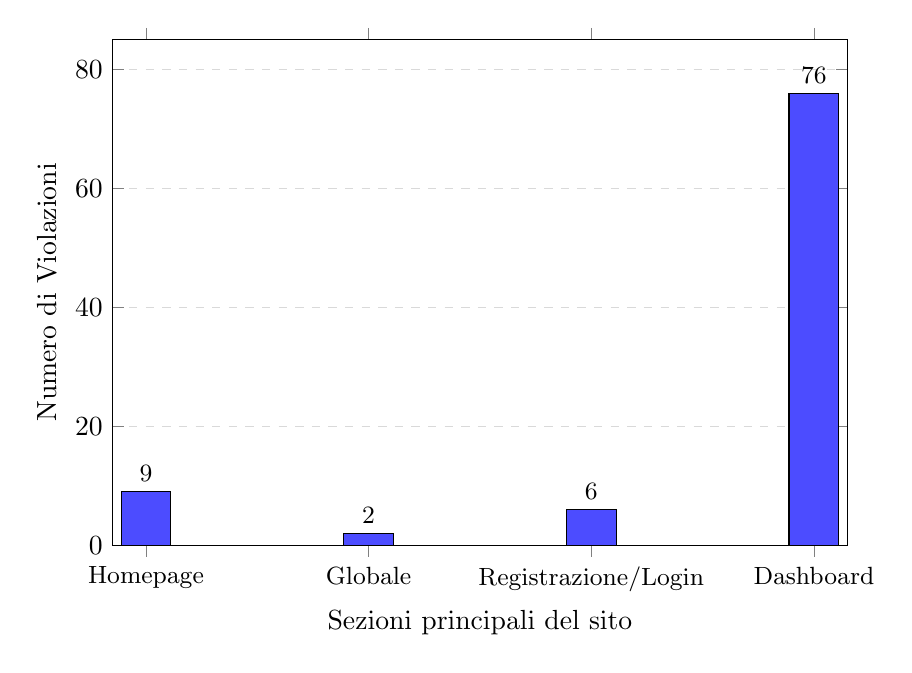
\begin{tikzpicture}
    \begin{axis}[
        ybar,
        bar width=18pt,
        width=0.9\textwidth,
        height=8cm,
        symbolic x coords={P1, P2, P3, P4},
        xtick=data,
        xticklabels={Homepage, Globale, Registrazione/Login, Dashboard},
        x tick label style={font=\small},
        xlabel={Sezioni principali del sito},
        ylabel={Numero di Violazioni},
        ymin=0,
        ymax=85,
        ymajorgrids=true,
        grid style={dashed, gray!30},
        enlarge x limits=0.05,
        nodes near coords,
        every node near coord/.style={font=\small, color=black},
      ]
      \addplot+[ybar, fill=blue!70, draw=black] coordinates {
        (P1,9)
        (P2,2)
        (P3,6)
        (P4,76)
      };
    \end{axis}
  \end{tikzpicture}
  \caption{Classificazione dei problemi riscontrati per sezione di appartenenza.}
  \label{fig:violazioni-sezioni-sito}
\end{figure}

Come si può osservare, la \textit{Dashboard} presenta il numero più elevato di violazioni, con ben 76 problematiche identificate, rappresentando così l'area più critica del sito in termini di usabilità.
La \textit{Homepage} registra 9 violazioni, posizionandosi come la seconda sezione più problematica, sebbene con un numero significativamente inferiore rispetto alla \textit{Dashboard}.
Le sezioni di \textit{Registrazione/Login} presenta 6 violazioni, mentre a livello \textit{Globale} risultano esserci solo 2 violazioni rilevate.
La marcata differenza tra il numero di violazioni nelle sezioni della \textit{Dashboard} e nelle altre sezioni suggerisce che questa area del sito, caratterizzata da una maggiore complessità funzionale e interattiva, richiede un'attenzione particolare per garantire un'esperienza fruibile e usabile da tutti gli utenti. \\

\noindent
Considerato che la \textit{Dashboard} rappresenta la sezione del sito con il maggior numero di violazioni rilevate, si è reso necessario un approfondimento più dettagliato di quest'area. Per questo motivo, è stato elaborato un ulteriore grafico che suddivide e analizza la distribuzione dei problemi di usabilità all'interno delle singole sezioni che la compongono.

\begin{figure}[H]
  \centering
  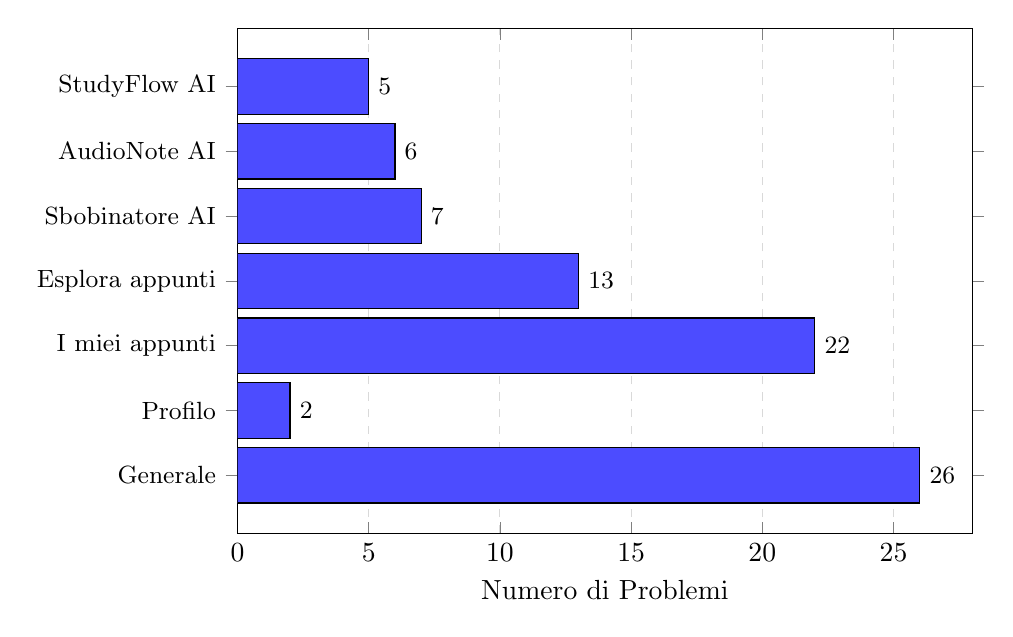
\begin{tikzpicture}
    \begin{axis}[
        xbar,
        bar width=20pt,
        width=0.9\textwidth,
        height=8cm,
        symbolic y coords={S0, S1, S2, S3, S4, S5, S6},
        ytick=data,
        yticklabels={Generale, Profilo, I miei appunti, Esplora appunti, Sbobinatore AI, AudioNote AI, StudyFlow AI},
        y tick label style={font=\small},
        xlabel={Numero di Problemi},
        xmin=0,
        xmax=28,
        xmajorgrids=true,
        grid style={dashed, gray!30},
        enlarge y limits=0.15,
        nodes near coords,
        every node near coord/.style={font=\small, color=black},
      ]
      \addplot+[xbar, fill=blue!70, draw=black] coordinates {
        (26,S0)
        (2,S1)
        (22,S2)
        (13,S3)
        (7,S4)
        (6,S5)
        (5,S6)
      };
    \end{axis}
  \end{tikzpicture}
  \label{fig:problemi-Dashboard}
  \caption{Distribuzione dei problemi di usabilità rilevati nelle diverse sezioni della Dashboard.}
\end{figure}

Come si può osservare, la sezione \textit{I miei appunti} presenta il numero più elevato di violazioni, con ben 22 problematiche identificate, rappresentando così l'area più critica dell'applicazione in termini di usabilità.
I problemi di natura generale, che interessano trasversalmente l'intera piattaforma, ammontano a 26 violazioni, costituendo una categoria significativa che richiede interventi sistemici.
La sezione \textit{Esplora appunti} registra 13 violazioni, posizionandosi come la terza area più problematica, seguita dalle funzionalità AI: \textit{Sbobinatore AI} con 7 violazioni, \textit{AudioNote AI} con 6 e \textit{StudyFlow AI} con 5.
La sezione \textit{Profilo} risulta essere la meno problematica tra le pagine specifiche, con sole 2 violazioni rilevate.
La marcata concentrazione di problematiche nella sezione \textit{I miei appunti} e nei problemi generali suggerisce che queste aree, caratterizzate da una maggiore complessità funzionale e da un impatto trasversale sull'esperienza utente, richiedono un'attenzione particolare per garantire un'esperienza fruibile e usabile da tutti gli utenti.


--------------------------------------------------------------
\begin{figure}[H]
  \centering
  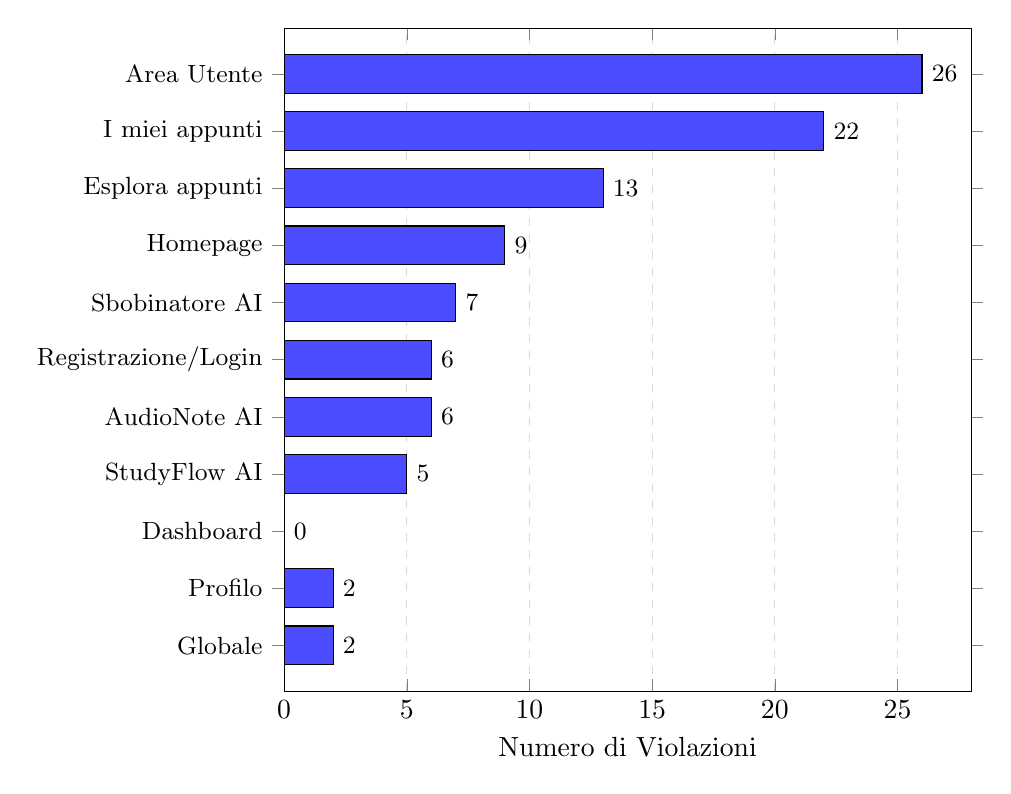
\begin{tikzpicture}
    \begin{axis}[
        xbar,
        bar width=14pt,
        width=0.85\textwidth,
        height=10cm,
        symbolic y coords={
          Globale,
          Profilo,
          Dashboard, % <-- Da aggiornare con il valore reale
          StudyFlow AI,
          AudioNote AI,
          Registrazione/Login,
          Sbobinatore AI,
          Homepage,
          Esplora appunti,
          I miei appunti,
          Area Utente
        },
        ytick=data,
        y tick label style={font=\small},
        xlabel={Numero di Violazioni},
        xmin=0,
        xmax=28,
        xmajorgrids=true,
        grid style={dashed, gray!30},
        enlarge y limits=0.08,
        nodes near coords,
        nodes near coords align={horizontal},
        every node near coord/.style={font=\small, color=black},
      ]
      % I dati sono inseriti dal più piccolo al più grande per far apparire 
      % la barra più lunga in alto nel grafico
      \addplot+[xbar, fill=blue!70, draw=black] coordinates {
        (2,Globale)
        (2,Profilo)
        (0,Dashboard) % <--- INSERISCI QUI IL NUMERO DI PROBLEMI DELLA VERA DASHBOARD
        (5,StudyFlow AI)
        (6,AudioNote AI)
        (6,Registrazione/Login)
        (7,Sbobinatore AI)
        (9,Homepage)
        (13,Esplora appunti)
        (22,I miei appunti)
        (26,Area Utente)
      };
    \end{axis}
  \end{tikzpicture}
  \caption{Distribuzione completa dei problemi di usabilità per sezione del sistema.}
  \label{fig:violazioni-complete}
\end{figure}

L'analisi della distribuzione fisica delle criticità è stata consolidata in un'unica vista complessiva (Figura \ref{fig:violazioni-complete}), permettendo di mappare l'incidenza dei problemi sull'intera architettura informativa del sistema, dall'area pubblica fino alle specifiche funzionalità dell'area personale.

Come si evince chiaramente dal grafico, le violazioni non si concentrano prevalentemente su singole pagine isolate, bensì su elementi condivisi. La categoria \textit{Trasversale (Area Utente)} risulta essere la più critica con 26 problematiche: si tratta di difetti di usabilità (es. incongruenze nei menù di navigazione o mancate indicazioni di stato) che l'utente sperimenta costantemente muovendosi tra le varie sezioni del proprio spazio di lavoro. A questi si sommano 2 problemi di natura puramente \textit{Trasversale (Intero sito)}, presenti sia nell'area pubblica che in quella privata.

Passando all'analisi delle pagine specifiche, la sezione \textit{I miei appunti} emerge in assoluto come l'area funzionale più problematica, registrando ben 22 violazioni. Essendo il cuore operativo della piattaforma, questa concentrazione di errori rappresenta un grave ostacolo alla fluidità dell'esperienza utente. A seguire si posiziona la sezione \textit{Esplora appunti} (13 violazioni), legata alle dinamiche di esplorazione e interazione con la community. 

Risulta interessante notare come l'area pubblica pre-login (\textit{Homepage} con 9 violazioni e \textit{Registrazione/Login} con 6) e le funzionalità avanzate basate sull'Intelligenza Artificiale (\textit{Sbobinatore AI}, \textit{AudioNote AI} e \textit{StudyFlow AI}) si assestino su valori medi, compresi tra 5 e 9 problematiche ciascuna. Infine, la pagina \textit{Profilo} e la \textit{Dashboard} riassuntiva [modifica questa frase in base al numero di problemi della dashboard] si confermano come gli ambienti più stabili e privi di frizioni del sistema.

Questa marcata polarizzazione suggerisce che gli interventi di riprogettazione dovranno concentrarsi prioritariamente sull'armonizzazione dei pattern visivi e navigazionali dell'intera area privata e, nello specifico, sul flusso di gestione dei propri documenti.
